%%
%% This is file `example.tex',
%% generated with the docstrip utility.
%%
%% The original source files were:
%%
%% coppe.dtx  (with options: `example')
%% 
%% This is a sample monograph which illustrates the use of `coppe' document
%% class and `coppe-unsrt' BibTeX style.
%% 
%% \CheckSum{1613}
%% \CharacterTable
%%  {Upper-case    \A\B\C\D\E\F\G\H\I\J\K\L\M\N\O\P\Q\R\S\T\U\V\W\X\Y\Z
%%   Lower-case    \a\b\c\d\e\f\g\h\i\j\k\l\m\n\o\p\q\r\s\t\u\v\w\x\y\z
%%   Digits        \0\1\2\3\4\5\6\7\8\9
%%   Exclamation   \!     Double quote  \"     Hash (number) \#
%%   Dollar        \$     Percent       \%     Ampersand     \&
%%   Acute accent  \'     Left paren    \(     Right paren   \)
%%   Asterisk      \*     Plus          \+     Comma         \,
%%   Minus         \-     Point         \.     Solidus       \/
%%   Colon         \:     Semicolon     \;     Less than     \<
%%   Equals        \=     Greater than  \>     Question mark \?
%%   Commercial at \@     Left bracket  \[     Backslash     \\
%%   Right bracket \]     Circumflex    \^     Underscore    \_
%%   Grave accent  \`     Left brace    \{     Vertical bar  \|
%%   Right brace   \}     Tilde         \~}
%%
% useful link: https://apgita.org.br/academico/teses-e-latex/
\documentclass[msc,numbers,english]{coppe} % maybe mscexam?
\usepackage{amsmath,amssymb}
\usepackage{hyperref}
\usepackage[table]{xcolor}
\usepackage{array}
\usepackage{multirow}
\usepackage{multicol}
\usepackage{algorithm}
\usepackage{pythonhighlight}
\usepackage[noend]{algpseudocode} 
\usepackage{multirow}
\usepackage{nicefrac}
\usepackage{multicol}
\usepackage{dirtytalk}
\usepackage{float}
\newcolumntype{P}[1]{>{\centering\arraybackslash\hspace{0pt}}p{#1}}
\interfootnotelinepenalty=10000

\makelosymbols
\makeloabbreviations

\begin{document}
% \title{Tradução automática através de redes neurais em domínios de baixo recurso: uma análise ponta a ponta do caso do português brasileiro}
% \foreigntitle{TACKLING LOW-RESOURCE NEURAL MACHINE TRANSLATION: ANEND-TO-END ANALYSIS FOR A BRAZILIAN PORTUGUESE CASE STUDY}
% Modelos neurais profundos para tradução em cenários de baixo recurso: um caso de estudo Português-Inglês 
\title{Modelos neurais profundos para tradução em cenários de baixo recurso: um estudo de caso Português-Inglês}
\foreigntitle{Deep learning models applied to machine translation under low-resource settings: a Portuguese-English case study}
\author{Arthur}{Telles Estrella}
\advisor{Prof.}{João}{Baptista de Oliveira e Souza Filho}{D.Sc.}
% \advisor{Prof.}{Nome do Segundo Orientador}{Sobrenome}{Ph.D.}
% \advisor{Prof.}{Nome do Terceiro Orientador}{Sobrenome}{D.Sc.}

% \examiner{Prof.}{João}{Baptista de Oliveira e Souza Filho}{D.Sc.}
% \examiner{Prof.}{Nome do Segundo Examinador Sobrenome}{Ph.D.}
% \examiner{Prof.}{Nome do Terceiro Examinador Sobrenome}{D.Sc.}
% \examiner{Prof.}{Nome do Quarto Examinador Sobrenome}{Ph.D.}
% \examiner{Prof.}{Nome do Quinto Examinador Sobrenome}{Ph.D.}
\department{PEE}
\date{05}{2022}

\keyword{Tradução automática}
\keyword{Aprendizado profundo}
\keyword{Processamento de linguagem natural}
\keyword{Aprendizado de máquina}
\keyword{Redes neurais}

\maketitle

\frontmatter

\dedication{Dedico este trabalho a minha família, principalmente meus pais Luciene e Guilherme e ao meu amor, Débora}

\chapter*{Agradecimentos}

Agradeço ao empenho dos meus pais em me orientar pelos caminhos corretos. Eles foram responsáveis por me incentivar a entrar em uma busca interminável por conhecimento, e que me levou a alcançar essa conquista. Agradeço ao carinho, bons valores e conforto que foram sempre prioridades da minha tia Sueli (\textit{in memoriam}), avó Sidnéia (\textit{in memoriam}) e Tia Maria (\textit{in memoriam}). Agradeço também ao meu avô Leonídio (\textit{in memoriam}), que serviu de exemplo de que o trabalho pode render grandes frutos, independentemente do nível de conhecimento com que se começa. Homenageio também minha irmã pela parceria disponível a qualquer momento.

Sou grato ao professor João Baptista Filho pela inserção no mundo de estatística e aprendizado de máquina, pela sua orientação que já dura desde os primeiros passos da graduação e alto valor agregado em importantes decisões tomadas durante o curso desta dissertação. Agradeço às experiencias de trabalho privado que tive e especialmente aos meus principais mentores durante essa trajetória. Estes foram responsáveis por me capacitar e revelar diversas oportunidades, abrindo incontáveis portas e contribuindo para o profissional que sou hoje.

\begin{abstract}

% estabelecer cenários de avaliação
% clusterização
% nas tecnicas, explicar primeiro e citar depois as tecnicas
% existem tecnicas para dominios de baixo recurso, como xyz, mas os vieses não foram amplamente estudados
% trocar discutidos com comparados
% trocar 
% mesmo onde há limitação em conjuntos de dados ou restrições quanto ao consumo de energia
% sem aplicar o esforço de extrair varias bases de dados 

Com o avanço das técnicas de processamento de linguagem natural que utilizam aprendizado profundo, os modelos de tradução automática ganharam espaço, porém os erros produzidos por esses modelos são pouco explorados ou explicados. O problema se agrava ao usar poucos dados para treino (low-resource), devido à uma limitação de vocabulário. Existem técnicas para lidar com as limitações de domínios de baixo recurso, tais como subword embeddings, pre-trained word embeddings e back translation; mas os vieses inseridos por elas na tradução não foram amplamente estudados. Esta dissertação se diferencia dos trabalhos trabalhos mais recentes, que normalmente focam em aumentar o BLEU score, negligenciando os erros produzidos por estes modelos durante o processo. Propõe-se técnicas qualitativas e quantitativas de avaliação, utilizando testes de hipótese e ferramentas de aprendizado de máquina para avaliar os vieses de um modelo de tradução, submetido a baixa disponibilidade de dados e treinado em uma única GPU. O estudo é focado no par português-inglês e BLEU é usado como métrica referência para a avaliação da parte quantitativa. Uma análise qualitativa é conduzida junto com um tradutor humano para entender os padrões de erros em frases e complementado com uma estratificação de diferentes níveis de complexidade (usando a escala CEFR) para entender a correlação entre estas variáveis. Modelos Transformer são usados e comparados com um referencial, o Google Translate, para avaliar o compromisso entre custo computacional e performance. O melhor modelo de baixo recurso desenvolvido é capaz de atingir 40.26 BLEU, correspondendo a 77.1\% do obtido pelo Google Translate (01/2022). Esse resultado reforça o potencial de uma abordagem eficiente low-resource em alcançar performance similar a modelos complexos no estado da arte, mesmo com restrições de dados e limitado custo financeiro e energético.

\end{abstract}

\begin{foreignabstract}

Neural Machine Translation models have flourished with the advance of Deep Learning Techniques and Natural Language Processing techniques, however, the errors produced by these models are little explored or explained. This issue aggravates when using a small dataset for training (low-resource), leveraged by a vocabulary limitation. There are techniques available to deal with low-resource domain limitations in the context of Machine Translation, like subword embeddings, pre-trained word embeddings and back translation; but the bias inserted by them in translations hasn't been widely studied. This dissertation differs from recent works, that usually focus on increasing BLEU score, overlooking the errors produced by the models during this process. We propose qualitative and quantitative evaluation frameworks, using hypothesis tests and machine learning tools for the qualitative approach to evaluate the biases of the translation model, exposed to low data availability and trained on a single GPU. The study focuses on the Portuguese-English pair, and BLEU is used as a benchmark metric to evaluate the quantitative. A qualitative analysis is conducted along with a human translator to understand error patterns in sentences and is also complemented with a stratification of different complexity levels (using the CEFR scale) to understand the correlation between them. Transformer-based models are used and compared to a benchmark model, Google Translate, to evaluate the balance between resource efficiency and performance. The best model built is capable of reaching 40.26 BLEU, 77.1\% of what the Google Translate benchmark achieved (01/2022). This result reinforces the potential of using efficient low-resource approaches to reach a performance similar to the high complexity state-of-the-art models, even with constrained data availability and reduced budget for energy and infrastructure.

\end{foreignabstract}

\tableofcontents
\listoffigures
\listofalgorithms
\listoftables
% --- UNDERSTAND HOW TO USE THIS ---
\printlosymbols
\printloabbreviations
% \listabbreviationname
% ----------------------------------
\mainmatter
\chapter{Introduction}
\section{The reenactment of Machine Translation}

Machine translation \abbrev{Machine Translation}{MT} is a research field that until 2013 has mainly invested in statistical based models, but the breakthrough promoted by sequence to sequence algorithms followed by the use of Transformer models has significantly changed the focus of the field. Before neural networks, Machine Translation systems were rule-based, syntax-based, phrase-based or a blend between more than one of these techniques. Probabilistic models used to be considered the state-of-the-art before the sequence to sequence paper. The increase in performance promoted by the sequence to sequence and Transformers received some attention, and soon other variants were developed.

The challenge of translating text got constrained by computational power issues for many years, until the rise of Transformers, which turned possible to perform the high amount of computation required in these cases in a truly parallel schema. With this new architecture, the operations performed during training are not totally dependent, allowing them to be parallelized in Graphic Processing Units (GPUs). Thus, by removing the constraint that some operations must wait for others to finish, NMT \abbrev{NMT}{Neural Machine Translation} models could scale largely and reach higher quality translations.

Just in 3 years, NMT became the dominant approach to Machine Translation, inducing a major transition from statistical to neural models.

\section{Challenges for the Portuguese language}
\label{portuguese_challenges}

Traditionally, the Machine Translation datasets and related conferences usually focus on languages from countries that are actively investing on NLP, which biases and narrows the potential of such algorithms towards a specific domain. Unfortunately, Portuguese is a language that does not dispose of supervised translation data in diversity and quantity. This issue increases the struggle to build a model that can successfully translate text in this idiom to other languages. Another obstacle are the european, brazilian and african Portuguese variants. Leading to a challenge for the model since generalization becomed hard if several sentences with different dialects can have the same meaning. We have performed an extensive search for works with a qualitative analysis of translation results for brazilian Portuguese, and only one single paper was found \cite{Caseli2020NMTAP}, indicating a vast unexplored terrain when considering translation errors in Machine Translation.

The branch of NMT inside the big topic of natural language processing is also a field with few papers and academic works among many Brazilian universities. This can be partially explained by the challenge that this environment imposes over practitioners: most models require cutting edge GPUs and usually only one GPU is not enough for medium-sized models on an average WMT competition dataset. The scarcity of these resources for many researchers require them to innovate in a limited domain and search for cloud solutions without sponsorship.

Finally, Portuguese is a complex language that uses accents which can change their meaning (\textit{e.g.} "e" and "é"), has different pronoun placements (\textit{e.g.} "realizar-se-á" equals "se realizará") and irregular verb inflections (\textit{e.g.} the "pôr" and "haver" verbs) so text preprocessing and tokenization plays an important role. Disregarding these details by applying some generic preprocessing steps that eliminates accents, for instance, can lead to a worse model performance. On the other hand, exploiting some domain knowledge on NLP often helps the model to better translate or classify, depending on the task at hand.

\section{Contributions of this dissertation}

Many previous works for solving the NMT task have focused on surpassing the state-of-the-art, disregarding the associated computational burden for achieving this goal. The research under this scope is often solely driven by increasing scores such as BLEU, which have limitations in assessing the quality of the translations generated. This dissertation tries to be an initial effort in trying to fill this gap, in the sense that our focus is both on assessing quantitatively and qualitatively the translations automatically produced by a NMT model and the techniques that can be potentially associated with it, while considering resource efficiency under low-resource settings.

The motivation for the concentration on low-resource scenarios arises from the emergence of IoT applications, whose computing power is typically restricted. Besides, for most researchers, the task of developing a competitive translation model without a robust infrastructure is becoming increasingly hard over time. As the access to such machinery is restricted to a selected group of researchers, there is an active trend in the community of investing in accessible AI \abbrev{AI}{Artificial Intelligence}, whose one of the priorities is investing on experiments that could be performed using low-cost GPUs.

% In a scenario where performance is a matter of ultimate importance, the quality issues derived from model guesses and how specific techniques help to address some quality aspects are overlooked. Also, many researchers cannot take advantage of cutting-edge infrastructure or abundant data, so understanding efficient approaches that maintain a reasonable cost-benefit balance is key to succeed.

As a result of the effort put on this dissertation, we published a conference paper at Symposium in Information and Human Language Technology (STIL) \cite{portuguese-nmt}\footnote{The full paper is publicly available at \url{https://sol.sbc.org.br/index.php/stil/article/view/17807}.}. The paper reports our early work on exploiting resource efficient Natural Language Processing (NLP) \abbrev{NLP}{Natural Language Processing} techniques to leverage translation performance as well as analysing the quality of resulting translations, both quantitatively as qualitatively, in resource constrained environments, analysing with statistical hypothesis tests the translation error patterns. 

This work concentrates on the Transformers model \cite{DBLP:journals/corr/VaswaniSPUJGKP17}, currently the state-of-the-art in NLP, and experimentally evaluate to what extent techniques such as transfer learning, modelling of subsets of words (subword embedding), and dataset augmentation with artificial sentences (back translation) can leverage a NMT model excel in a low-resource environment. This experimental study is conducted with only one average size GPU and small to medium-sized datasets, considering the English-to-Portuguese pair. In a quantitative sense, the challenge of low-resource is emulated considering samples of the dataset with a range of sizes. The goal is to infer how cost-effective are the aforementioned techniques under such settings. A qualitative analysis is also conducted in the study, where clusters (characteristics) of errors are defined with the help of a Brazilian English translator. His participation was crucial to spot and classify mistakes in grammatical patterns and put them under well defined clusters. The translator also applies his knowledge to stratify the sentences using a complexity drill down, rated according to the CEFR scale \cite{COE}. The qualitative dimensions of sentence complexity and error patterns are subjected to 3 experiments that reveal the bidimensional associations between the model variants and these factors. In the end of the analysis we conclude that the techniques associated with the model indeed have an influence over the error patterns.

For comparison purposes, the model with the most promising score is compared with the Google Translate service, acessed by API \cite{gtranslate_api}, over the test set of the main datasets used. Despite the significantly higher but precisely unknown quantity of data as well as the level of human and computing efforts required for training the Google model, our low-resource model reached 77.1\% of the Google's model BLEU score.

This work is not only an attempt to explain qualitatively and quantitatively the pros and cons of applying a specific technique in low-resource environments. We also hope to stimulate the community to dive deeper into error patterns and biases of specific techniques in NMT, as our belief is that this process may aid on leading the community towards producing clearer, more fluid and grammatically correct translations.

\section{Dissertation Organization}

The fundamentals of NLP that are the pillars for NMT, such as types of word representations and how the translation task works are presented in Chapter 2. Chapter 3 introduces some sequence to sequence neural architectures: the Transformer and Recurrent Neural Network (RNN) \abbrev{RNN}{Recurrent Neural Network}, along with some interesting properties that helped them to learn richer word representations and output more coherent translations.

In Chapter 4, aspects of low-resource domains and related constraints are outlined, along with a brief review of NLP techniques that can potentially help to reduce their side-effects on models' performance. A description of the datasets used in this work is provided in Chapter 5, which also depicts quantitative and qualitative experiments and corresponding results for the strategies considered. Finally, in Chapter 6 we derive some conclusions and outline further possible improvements and study directions. 

\chapter{A brief introduction to Natural Language Processing}

Natural language was considered by the Machine Learning community as one of the most complex data types to represent. Practical applications with meaningful feature representations took time to evolve, even longer than computer vision related tasks, which also required customized representations. In the sections below, a brief introduction to the different kinds of features used for word representations will be given to contextualize the reader of some of the historical challenges and evolution faced by this field.

\section{Feature representation}

Natural language can be represented either by words or tokens. The scope of tokens includes not only words, but also punctuation marks, acronyms and any other text that can be used as a placeholder. Despite that subtle distinction, both terms are used almost interchangeably when speaking of natural language representation in the literature. When referring to words or tokens throughout the next sections, we will be considering any of these sorts of natural language manifestation.

In order to keep the unique and original meaning of each word, one of the oldest and most popular ways to represent natural language is through one-hot encoding. Let $V$ be the number of distinct words present in a vocabulary. When this set of words is vectorized, each word will be represented by an unique not-null dimension inside a binary vector of size $V$. In other words this means that when representing one word, the vector contains 1 for the dimension of that word and all the other positions are filled with zeroes. Thus, the vectors of two different words would be considered orthogonal, i.e. have their dot product equal to 0, not allowing any measure of similarity between them. One-hot encoding is a type of sparse representation, which has only one position different than zero. Another method disadvantage is employing a high number of dimensions to represent even small and medium-size vocabularies, imposing relevant challenges to algorithms that cannot properly handle high-dimensional inputs.

Another possibility to represent a set of input words is using fixed-length real vectors, where the number of dimensions is pre-specified, regardless the vocabulary size. These real numbers may widely vary in range depending on how there are generated, and there is a number of techniques that can provide them. For instance, such vectors can be randomly initialized using uniform distributions and then adjusted using an optimization algorithm based on statistics over the co-occurrence of words. In the most simple neural-based algorithms, such real number vectors are usually extracted from the weights related to the first network layer, thus can be referred to as weight vectors or neural embedding. This word encoding strategy is also known as dense representation.

There are pros and cons for using either sparse or dense vectors to represent words. A brief summary can be found at Table \ref{feature-representations}.

\begin{table}[h]
\caption{Pros and Cons per Feature Representation}
\fontsize{10}{12}\fontfamily{phv}\selectfont
\label{feature-representations}
\centering
  {\footnotesize
  \begin{tabular}{| p{0.15\linewidth} | P{0.12\linewidth} | P{0.09\linewidth} | P{0.18\linewidth} | P{0.32\linewidth} |}
    \hline
    Feature representation & Encoding Type & Dimensionality & Information sharing & Curse of dimensionality \\
    \hline
    One-hot encoding & Sparse & High & None, as the vector dimensions are independent & Sparse and high-dimensional vectors may hinder model performance \\
    \hline
    Neural embedding & Dense & Fixed-Length & Similar vectors (low cossine angle) for related words & Dimensionality can be experimentally tuned to a sweet spot \\
    % \hline
    % BT (50\% of News synthetic examples) & 34 & 33 & 21.80 & 51.34\\
    \hline
\end{tabular}}
\end{table}
  
We should stress that if the dimension is too high in one-hot encoding, some dimensionality reduction may be applied. However, depending on the dataset and the algorithm considered, this process may be contraindicated due to the computational requirements involved, as potential quality issues may arise. On the other hand, the weight encoding alternative lets you tune the embedding dimension, but this may require several experiments to achieve an optimal performance. The algorithm used to generate the embeddings also plays an important role in this process.
  
\section{Neural word embeddings}
\label{neural_embedding}

Natural language representation using neural word embeddings was responsible to allow Machine Learning algorithms scale to a range of applications, representing a watershed for the research community. Neural networks can be recognized as intrinsic dense vector learners, due to the weight update operations performed during forward and backpropagation. In a neural network capable of modelling words, the weights themselves when concatenated into a vector can be optimized to represent a specific word.

\begin{figure*}[tb]
\centering 
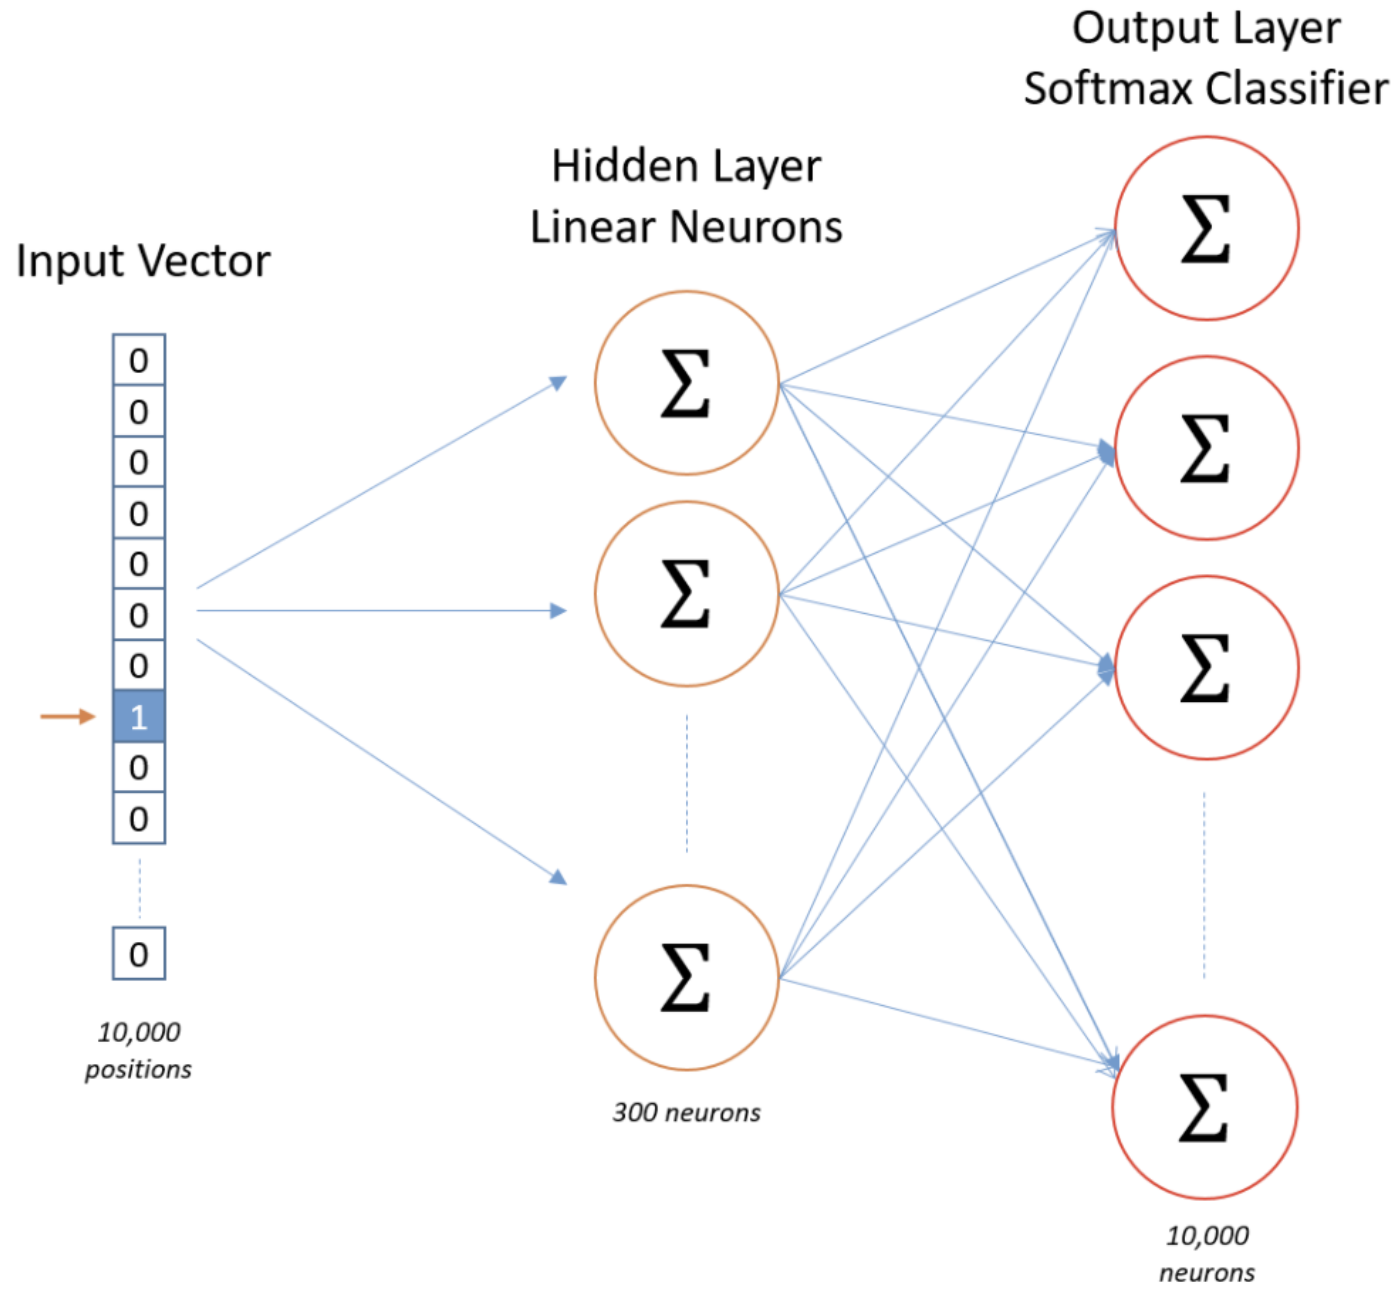
\includegraphics[keepaspectratio,scale=0.4]{chapter2_images/word2vec_didatic.png}
\caption{Architecture diagram for calculating word probabilities using a 2-layer Neural Network.}
\label{word2vec_didatic_architecture}
\end{figure*}

The properties of each modality of feature representation previously reported in Table \ref{feature-representations} are clear, but one question remains: How dense vectors are able to capture the similarity in meaning between words? One quote by John Firth from 1952 may shed light on the potential answer:\newline

\say{You shall know a word by the company it keeps.} \newline

Basically, the meaning of a word can be defined by the context around it, and usually this context is extracted using a fixed-size window, whose size is a hyperparameter of the algorithm, here denoted as $c$. To gradually understand how words relate to their context, let us first consider the association between two arbitrary words in a sentence.

\subsection{Single-word context}

One popular technique to obtain word weights is the two-layer neural network architecture illustrated at Figure \ref{word2vec_didatic_architecture}. It is a simplified representation of a neural word embedding, taking an one-hot encoded vector $\mathbf{v}$ of size $v$ as input and generating a dense vector at the outputs of its hidden layer neurons. In this case, the weights between the input vector and the hidden layer can be represented by a $v \times n$ matrix $\mathbf{W}$, where $n$ and $v$ are the and the vocabulary sizes, respectively. Therefore, each row of $\mathbf{W}$ is a $n$-dimensional vectorial representation $\textbf{v}_{w}$ of the respective word in the dictionary (here all vectors are assumed as column vectors). This enables the hidden layer to become analogous to a lookup table, where each row represents a different word.

In Figure \ref{word2vec_didatic_architecture}, the hidden layer outputs are simply defined by $\mathbf{h}=W^{T}\mathbf{x}$. From the hidden layer to the output layer, there is another weight matrix $\mathcal{W}^{'}=\textbf{w}^{'}_{Cj}$, with dimensions $n \times v$. Weights from both matrices can be used to compute scores $\textbf{u}_{j^{'}}$ and $\textbf{u}_{j}$ for a given word:

\begin{equation}
\textbf{u}_{j^{'}} = \textbf{v}^{'T}_{w_{j}}\mathbf{h}, 
\label{input_hidden}
\end{equation}
and 
\begin{equation}
\textbf{u}_{j} = \textbf{v}^{T}_{w_{j}}\mathbf{h},
\label{hidden_output}
\end{equation}
where $1 \le j \le v$, while $\textbf{v}^{'T}_{w_{j}}$ and $\textbf{v}^{T}_{w_{j}}$ are the $j$-th column of the matrix $\mathbf{W}^{'}$ and $\mathbf{W}$, respectively. Now, consider the following problem: What is the most likely word that succedes a given word? Assuming the network is trained, one may just set the corresponding $v_{x}$ to this word, generate the corresponding embedding $h$, and apply $h$ to output layer to infer the likelihood of each vocabulary word in succeeding it. Before the likelihood inference, the score of \ref{hidden_output} is then passed through a softmax layer, that calculates the probability of a set of words that could be fit into that context.

In this case, the output layer is responsible for inferring the level of association of a word with another word in its context (in this example, the word succeeding it), or vice versa, depending on the approach used. Thus, the probability associated with each vocabulary word given a single word is given by the softmax function as follows:

\begin{equation}
\label{softmax_output}
p(w_{o}|w_{j}) = \frac{exp(\textbf{u}_{j})}{\sum^{v}_{j^{'}=1}exp(\textbf{u}_{j^{'}})},
\end{equation}
where $w_o$ denotes an arbitrary word from the vocabulary, $w_j$ is the current word, and $\textbf{u}_{j^{'}}$ and $\textbf{u}_{j}$ are given by \ref{input_hidden} and \ref{hidden_output}, respectively. 

\subsection{Multi-word context}

Better embeddings may be achieved by considering context windows composed of multiple words instead a single one. Figure \ref{word_window} illustrates some examples. Now consider that the central word is immersed in a context of $C$ other words, where $c=\frac{C}{2}$. As the output word $o$ lies within the target word's context, it can also be denoted by $i+o$, with $o$ being the number of positions ahead or behind the input inside the text and $i$ is the position of the center word.

\begin{figure*}[b]
\centering 
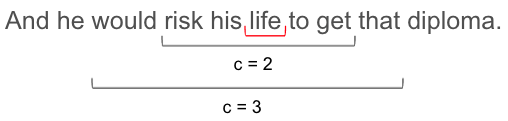
\includegraphics[keepaspectratio,scale=0.6]{chapter2_images/word_window.png}
\caption{Word context window of sizes 2 and 3}
\label{word_window}
\end{figure*}

The idea here is the same as before: starting the weights of the word embedding randomly and updating them based on how they interact with nearby words, using an optimization algorithm. For the sake of simplicity, such iterations will be simply evaluated by quantifying the pairwise associations (\textit{i.e.} between the word and those integrating the context window), in terms of the likelihood that both words might co-occur. Therefore, the model's task is calculating the probability of a surrounding word $w_{i+o}$ given a word $w_{j}$, denoted as $p(w_{i+o}|w_{i})$. Once all the words in the context of a center word are defined by the length of the fixed window, the goal is to maximize the likelihood of the context words given the center word. Assuming a multiple independence between the multiple pairs of central and context words, the likelihood function to be maximized is given by:

\begin{equation}
\label{maximize_likelihood}
L(\theta) = \prod^{C}_{i=1} \prod_{\substack{-c \leq o \leq c \\ o \neq 0}} P(w_{i+o} | w_{i}).
\end{equation}

The same equations previously presented also apply for the multi-word case. The difference is that now \ref{input_hidden} and \ref{hidden_output} are calculated for each surrounding word, and Equation \ref{softmax_output} is applied using a sliding window approach, where the surrounding words represent the context of the window.

% words vary in -c<j<c
% units in vector very in 0<v<V
% https://medium.com/analytics-vidhya/maths-behind-word2vec-explained-38d74f32726b

\subsection{\mbox{Word2Vec}: CBOW and Skipgram}

The explanation so far constitutes a simplified version of the architecture proposed in the seminal work of \citet{mikolov2013efficient}, popularly known by the alias of \mbox{Word2Vec}. In the original proposal, it operates in a multi-word setting, which in turn has 2 variations: Continous Bag of Words (CBOW) \abbrev{CBOW}{Continous Bag of Words}, whose rationale is ilustrated by the left side of Figure \ref{cbow_skipgram}, and Skipgram, on the right. The main difference between them is that in CBOW, the task performed consists in predicting the target word based on the context, while in Skipgram the context words are predicted based on the central word. A more detailed explanation will be provided for Skipgram, since the embeddings exploited in this work will be based on it, and it has consolidated itself in the literature as a more effective approach for a wide range of experiments.

% One aspect of the CBOW variant model that changes when compared to the simplified architecture is that it takes the average of the vectors of the input context words, it takes the product of the input and hidden weight matrix, then calculates the average vector as the output.

% \textcolor{red}{Question: should I add the reference for the equations? Even if I changed the logical order and some of the variables used to present them?}
% its from word2vec parameter learning explained


Remember that our previous modelling approach constitutes of calculating the probability of the co-occurring the output word $o$ with the center word $i$, considering $-c \leq o \leq c$. In order to obtain the parameter update equations for this model, we need to maximize Equation \ref{softmax_output}. The loss function $E$ exploited for maximizing the context window in Skipgram is given by:

\begin{equation}
\label{skipgram_loss}
\begin{aligned}
E = & -\log p (w_{i+c}, w_{i+c-1}, \dots, w_{i+1}|w_{i}) \\
& = -\log \prod^{C}_{o=1} \frac{exp(u_{o^{*}_{c}})}{\sum^{V}_{j^{'}=1}exp(u_{j^{'}})} \\
& = -\sum^{C}_{o=1}u_{o^{*}_{c}} + C\times\log\sum^{V}_{j^{'}=1}\exp{u_{j^{'}}},
\end{aligned}
\end{equation}
where $o^{*}_{c}$ represents the output index of the current $c$-th context word in the vocabulary. This algorithm updates the word vectors for each element in the context, but the final representation of the word reflects its neighbors, since it is influenced by all of them during the optimization process. If interested in further details on how \mbox{Word2Vec} equations are derived, the reader is referred to \citet{DBLP:journals/corr/Rong14}. 

Equation \ref{softmax_output} also represents the output of the softmax function in Word2Vec and it is the pure form of the Skipgram embedding. An interesting analogy that helps to grasp the way this multi-word mechanism works is to think that the previously mentioned logistic regression neurons are trying to distinguish what a "true context" word is of what can potentially be "noise", an unrelated word in the text.

\begin{figure*}[tb]
\centering 
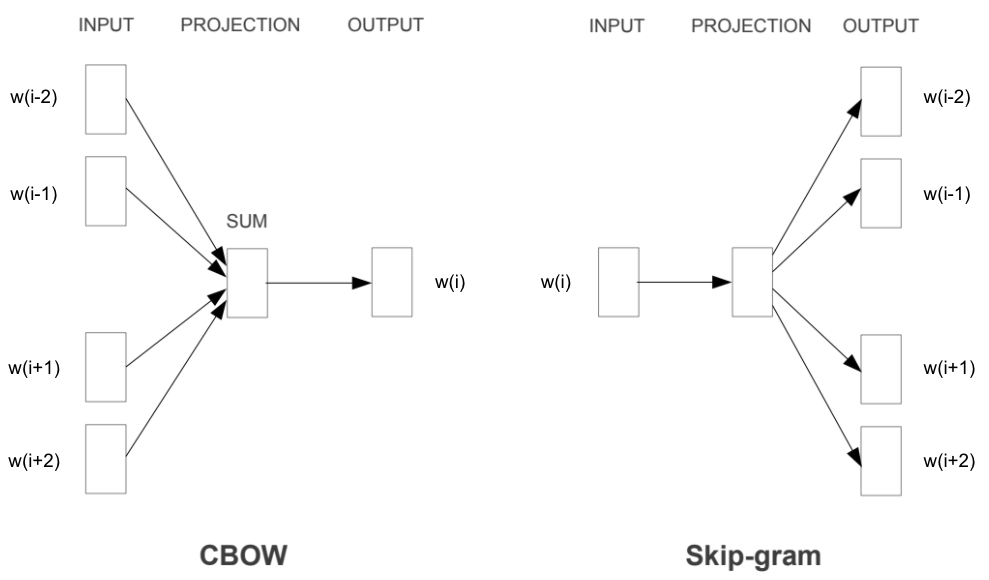
\includegraphics[keepaspectratio,scale=0.35]{chapter2_images/cbow_skipgram.png}
\caption{Multi-word mechanisms CBOW and Skipgram}
\label{cbow_skipgram}
\end{figure*}

In addition to the pure form, there are also some optimization tricks applied to improve its scalability: hierarchical softmax and negative sampling. The hierarchical version of softmax mitigates the expensive number of operations involved in computing the denominador of Equation \ref{skipgram_loss}, with a computing mechanism based on binary trees. In such trees, the leaves represent words and the calculation of a word probability is decomposed into a sequence of probability calculations. This saves the algorithm from having to calculate the expensive normalization over all words.

Another feature inserted in the implementation is negative sampling. Considering a context window where word $A$ and $B$ are being compared, the algorithm's goal is to approximate or move away their word vectors in a multidimensional space, and for this it has to consider the relation of the target word with other words. Usually all the other words in the vocabulary are used as spurious samples, which is computationally expensive, but negative sample provides an empirical statistical method to sample only a subset of these words. The output word (the most probable word) is kept in the sample and gets updated, and the negative samples are drawn following a probabilistic distribution that can be arbitrarily chosen. This distribution is called noise distribution, and to make sure that the selection of a good sample will be performed, an empirical methodology was applied by the authors. They define a simplified training objective that is capable of producing high-quality embeddings in their original paper \cite{mikolov2013efficient}. The probabilistic distribution used is based on a posterior multinomial distribution \cite{DBLP:journals/corr/Rong14}. Negative sampling and hierarchical softmax were crucial to enable a huge number of practical applications using Word2Vec, and have also attracted the attention of other Machine Learning branches. 
% https://ruder.io/word-embeddings-softmax/index.html#hierarchicalsoftmax

\section{Machine Translation and its challenges}
\label{machine_traslation_challenges}
% taken from chapter 10 of https://web.stanford.edu/~jurafsky/slp3/

Some aspects of the human language seem to be universal, or statistically universal, since we know only a subset of the languages that were created in the whole history of mankind in the current year of 2021. When speaking of language diversity, only widely spoken and recently created languages are considered. Many of these languages employ the use of verbs and nouns, words to refer to animals, emotions,  attitudes and other aspects. Yet, there are a number of differences between them. They can be idiosyncratic or systematic for instance. Idiosyncratic accounts for which words are usually combined and how common they sound together, since different languages are usually biased to distinct sets of words. Systematic represents the word order chosen, for example if the verb is usually put before the direct object or not. The study of systematic differences is called linguistic typology. These and other challenges imposed by language nuances discussed in this section are inspired by the Neural Machine Translation chapter of the unfinished book of \citet{nmt_nlp_speech_draft_book}, shared as a draft.

\subsection{Word order typology}

Languages differ in the way they order verbs, subjects and objects in simple declarative clauses. Some are considered SVO (subject-verb-object) \abbrev{SVO}{subject-verb-object}, their sentences start with the subject, the verb is put in the middle and ends with an object. Portuguese, Chinese and English are SVO languages, whereas German and Japanese are SOV (subject-object-verb) \abbrev{SOV}{subject-object-verb}. There are also VSO (verb-subject-object) \abbrev{SOV}{verb-subject-object} languages, such as Arabic and Irish.

One of the most challenging environments for a NMT model to execute the translation task happens when it has to translate from a language of one typology type to another, which luckily isn't the case in this work, as both languages are SVO.

\subsection{Morphological typology}

Regarding typology, languages can be categorized in 2 dimensions. The first is the number of morphemes per word: isolating languages like Vietnamese usually contain one morpheme (one enclosed meaning or reference to something) per word. They are simpler to deal with than polysynthetic languages, which may contain a variable number of morphemes per word. This classification isn't binary, though. Portuguese and English are somewhere in between both, but closer to isolating rather than polysynthetic. Both languages can add suffixes or prefixes that change the meaning: for instance happy is an adjective, but when united with "ness" becomes a noun "happiness".

The second dimension is to which degree the morphemes are segmentable. Languages can be agglutinative (clear boundaries between morphemes) such as Turkish; or fusional, such as Spanish, where the boundaries between the morphemes are unclear or lost. One example for this is the verbal inflection "comí" (I ate), where the morphemes "comer" and "yo" have lost their boundaries between each other. Portuguese and English are considered to be fusional, but not as much as other fusional benchmarks such as Classical Hebrew.

\subsection{Word alignment}
\label{word_alignment}

Alignment in the context of translating means how word correspondences are made between the reference (source language) and its translation (target language). The aforementioned typological properties substantially increase the complexity of alignment, specially for situations where distinct typologies must be matched. 

Not all words in the source or target language necessarily need to be aligned, sometimes the role of one word in a translation pair is just to maintain fluency, contributing to a correct sentence in terms of grammar. Figure \ref{alignment_types} contains 3 alignment examples, wherein the source language is on the left and the target is on top. From left to right, the first rectangle represents a simple one-to-one scenario, the second shows a many-to-many relation and the third, one-to-many, all of them considering the Portuguese-English pair. Note that the last scenario has one spurious word in the source language which had no alignment with the target translation.

\begin{figure*}[tb]
\centering 
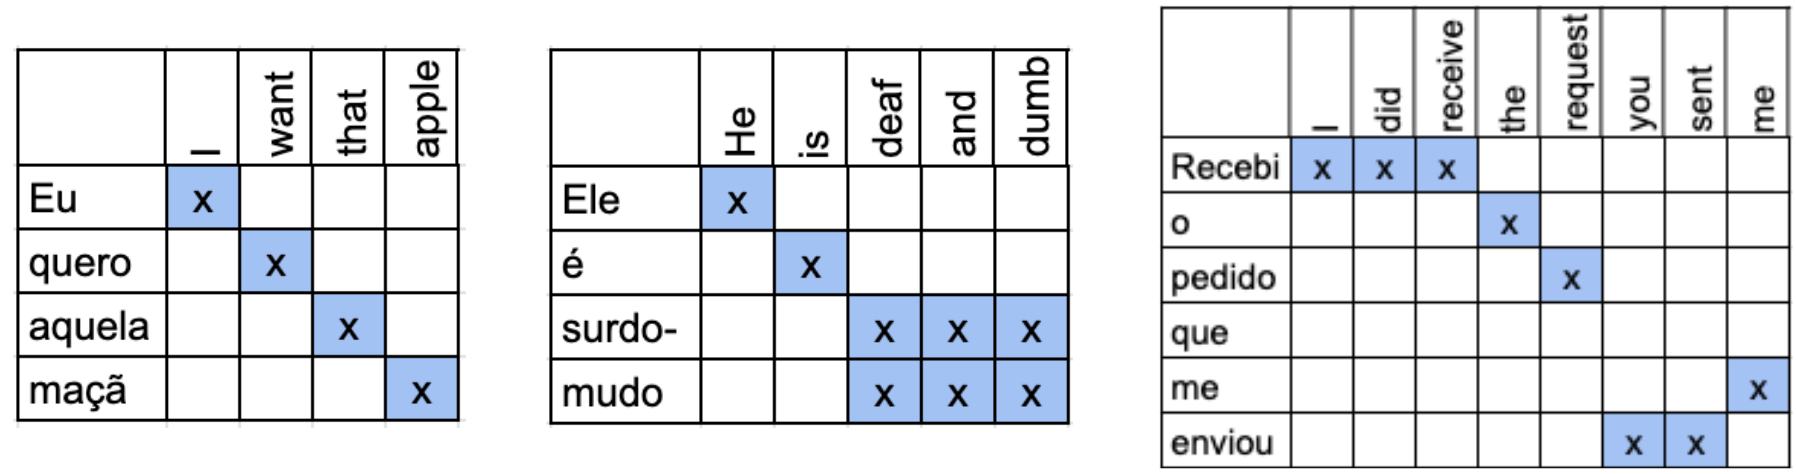
\includegraphics[keepaspectratio,scale=0.22]{chapter2_images/alignment_types.png}
\caption{One-to-one, many-to-many and one-to-many alignments using Portuguese and English sentences}
\label{alignment_types}
\end{figure*}

\subsection{Lexical divergences}

Sometimes, languages may contain a specific expression or word that cannot be accurately translated to another language without losing some of its meaning. Whenever this happens, the word constitutes a lexical gap between such languages. This is pretty common with slang words, which have a very specific use case, making it harder to express the same meaning in another language, even when using several words.

Another characteristic of languages that may increase the chance of happening a lexical gap is the fact that some of them are verb-framed. This means that they mark the path of motion in the verb and leave the satellites to express the manner of motion. The path of motion for instance means the direction of the movement, such as move into, out of or across, while the manner of motion refers to a specific type of motion, such as running, walking, or crawling. 

On the opposite side of verb-framed, there are languages that are satellite-framed, which means that the manner of motion is expressed in the verb while the path of motion is expressed in the satellite. As happened with other language characteristics, these classifications don't mean that a given language cannot mix verb-framed and satellite-framed expressions. English and Portuguese for instance can generate expressions using both styles. 

Consider the translation of language $A$ that mainly uses verb framing to language $B$, which mainly uses satellite framing. The difference in the framing pattern between $A$ and $B$ languages does not necessarily mean that the chance of lexical gaps increases. It means that $A$ may have a range of specificities by aggregating verbs that may be complex to reproduce with a correspondent aggregation of satellites in $B$. This diversity of patterns to generate distinct meaning might pose a challenge to generate an accurate translation, and may result in a partial loss of the original meaning.

\subsection{Qualitative aspects to evaluate translations}

Defining qualitative and quantitative characteristics for accurately evaluating how successful a translation was is hard. The quantitative matter will be further discussed in another section, but the qualitative side is usually broken into 2 dimensions, namely adequacy and fluency.

Adequacy represents how well the meaning of the source sentence was captured, and is sometimes referred to as fidelity. Synonyms hardly ever affect this dimension, and the complexity of correctly evaluating this dimension is what mostly hinders quantitative metrics. Fluency means how correct and fluid the translation is in the target language, it evaluates sentences in categories such as grammaticality, readability and naturality of the words chosen.

\subsection{Ambiguity}

The challenge of identifying and properly representing ambiguity is one of the most complex ones for natural languages. This happens because the model heavily depends on the diversity and quality of the dataset considered for its development, and it should be able to assign distinct features to different meanings. Ambiguity can be found at the word-level, for instance, the word sink can be a noun or a verb, which is known as lexical ambiguity. It can also occur for a whole sentence or a clause, then it is called structural ambiguity. Models inherently do not possess knowledge of the world to identify in which situations ambiguity may occur. 
If one could provide such knowledge to a model beforehand, than it should be capable of handling such situations, but no solution so far proved to be robust enough to achieve this.

A plausible critic for the effectiveness of the vector structure derived from \citet{mikolov2013efficient} is that it creates a single vector representation for words that may contain multiple meanings, hence capturing only the most frequent cases in the training set. It lacks flexibility to deal with occurrences of polysemy or homonymy in a given context. The word pike is a classic case of homonymy, also used to explain ambiguity in the course material of \citet{cs224n_stanford_l2}, since it can mean any of the following:

\begin{enumerate}
    \item A sharp edge or staff
    \item To piece or kill with a pike
    \item A type of elongated fish
    \item A railroad line or system
    \item One type of road
    \item To make one's way (pike along)
\end{enumerate}

There also other meanings this word can have based on your location in an English speaking country. Polysemy accounts for the coexistence of many possible meanings for a word or phrase, a phenomenon that happens in either Portuguese or English. In addition to the challenges of polysemy and homonymy, Portuguese provides some specific challenges such as distinct pronoun organizations that may carry the same meaning, and some others that were already mentioned in a previous section (\ref{portuguese_challenges}).

\subsection{The challenge of open vocabulary}
\label{open_vocabulary}

NMT models typically learn from supervised data, hence they are constrained to a fixed vocabulary. When dealing with an unseen word in some test scenario, traditional word-level models produce an $<unk>$ (unknown) token. This phenomenon is referred to as out-of-vocabulary (OOV) \abbrev{out-of-vocabulary}{OOV}. 

There are a number of ways to deal with the open vocabulary issue. Speaking of word-level models, the only way to reduce the chance for the model to produce $<unk>$ tokens is to guarantee that the training set has enough unique words to cover whatever words that appear for evaluation. One conclusion can be derived from this statement: the bigger the number of unique words a dataset has, the bigger the challenge of addressing open vocabulary becomes. Another observation to outline is that an increase in complexity and diversity of domains presented in the text for instance can be correlated with an increase of unique words. Some of the datasets used in this work corroborate with this hypothesis.

If the word-level restriction is removed, then subword models can increase the occurrence of smaller tokens, since they are capable of breaking the words into smaller units. These units can be characters (at the character-level), syllables or prefixes (at subword-level). By acting upon smaller pieces of the word, the model incorporates the ability of generating custom tokens, since any combination of these pieces become possible when generating translations.

\subsection{Addressing MT challenges}

This chapter performed an overview of the qualitative theory that is intrinsic to the study of natural languages, which is relevant to the context of Machine Translation. It sheds a light on the practical differences that one language may have when compared to another, and helps to understand some of the challenges that MT researchers faced when creating systems based on expert knowledge. Modelling all these nuances was a complex task, since many of the first MT systems were rule-based or phrase-based, belonging to a MT branch calling statistical Machine Translation. Specific language phenomena were compiled in a set of rules that was unique to each language pair, like tables of equivalent expressions, requiring a heavy manual effort to maintain and update such systems. The alignment, for instance, was treated by means of a latent variable. This hugely increased the complexity of the translation task, since the goal switched from predicting $P(x|y)$ to $P(x, a|y)$, where $a$ is the alignment variable.

Neural systems represented a breakthrough in this area, since they removed the manual work of modelling language nuances, learning them on their own. This came along with the flexibility to adapt their architecture given the available resources and performance target. Among other advantages of NMT are the better use of context and phrase similarities, enhanced fluency of the translations and the necessity to optimize only a single network end-to-end. NMT also has some disadvantages: neural networks are known for being a black-box algorithm which is very hard to interpret and debug. It is also difficult to control neural biases (which can be gender or race related) that depend on the dataset used and the process of learning as a whole.

Despite the disadvantages, the solid benefits motivated an investment in this research branch, increasing the number of publications of the field since 2014. Further technical details and practical behaviour of neural networks will be discussed in the following chapters.

\chapter{Neural networks and Machine Translation}

Since their ideation in 1958, Neural Networks have seen peaks and valleys of research interest in the Machine Learning field. They have gone out of the tar pit (term borrowed from \cite{Moseley2006OutOT} that originally mentioned learnings of "the dark times" in Software Engineering) in the 1980s with feedforward and recurrent variants, and evolved with contributions such as the convolutional and LSTM variants in 1990s. After such progress, they started to leverage promising results when applied to numerical and categorical data. Specially after 2013, Neural Networks were growing at an unseen rate, driven by the use of Deep Networks. Applications in image processing and natural language processing areas were massively explored and soon consolidated themselves as the state-of-the-art algorithms. 

Before going into further details of the pioneer research that applied Neural Networks to solve Machine Translation, the task of translating from one language to another will be formally explained. Even though are a few approaches to reach the same result, we will focus the core of the explanations on the neural alternative.

\section{Machine translation as a task}

The ability to use an automated procedure to translate from a source language to a target language had precursors since the 1930s, with the use of mechanical dictionaries, later coming up with some pioneer applications on the 1950s \cite{Hutchins1995MachineTA}. These applications were heavily funded by military and focused on Russian-English translation or the other way around, mostly motivated by the rivality between the United States and Soviet Union in the Cold-war period. Roughly, the translation task can be formulated as an optimization problem:

\begin{equation}
\label{translation_equation}
\hat{y} = argmax_{y} P (y | x),
\end{equation}
where $x$ is the representation of a sentence in the source language, $y$ represents another sentence in the target language, and $P$ is a probability value. Note that $P$ includes parameters to be trained using supervised learning. After training has been completed, these parameters will represent the model's word representation knowledge for a vocabulary previously seen. Based on this prior knowledge the model will generate its guess $\hat{y}$ for the sentence $x$. Using Bayes' theorem to decompose $P (y | x)$, the result would be the following:

% https://www.ee.columbia.edu/~sfchang/course/svia-F03/papers/brown-machine-translate-93.pdf
\begin{equation}
P(y|x) = \frac{P(y)P(x|y)}{P(x)}
\end{equation}

Since the denominator is independent of $y$, finding $\hat{y}$ is the same as to make the product $P(y)P(x|y)$ as large as possible. The following main components derived from this process are the representations of different challenges for the translation process: $P(x|y)$ and $P(y)$.

The probability indicated by $P(x|y)$ represents the translation model part, which is basically a mapping of which translation matches which source sentence, considering what the model has learned with the training set. Accordingly, $P(y)$ can be interpreted as a language model, basically responding for how fluently some meaning is defined using a set of words. To accurately reach a high probability for $P(x|y)$, a large amount of high-quality parallel data is required, whereas the other component $P(y)$ requires only proficiency under the scope of a single language (the target one).

Another approach to address this problem is to narrow the scope of the translation task by breaking it into more steps. This may be achieved, for instance, by introducing a latent variable $a$ that connects the source and target clauses and words. This variable is the mathematical representation of the alignment model described in a previous section \ref{word_alignment}, and it isn't explicitly specified in a dataset apriori. The alignment model basically connects particular words and positions between both languages.

The process of obtaining an efficient representation for $\hat{y}$ (the most probable translation guess) is performed with the help of a decoding algorithm. Decoding isn't a trivial task as it requires a robust algorithm to deal with both the translation and language models. Matching the reference with an algorithm is hard since human translators can reword a phrase with synonyms, reorder and rearrange words, replace single words with multi-word phrases, and vice versa. Decoding has also been proven as a NP-hard problem, even in relatively simple translation models \cite{knight-1999-decoding}. The task of reaching a degree of correspondence between source and target sentences is aggravated by the Machine Translation challenges covered in Section \ref{machine_traslation_challenges}.

When decoding the source sentence, there are some special tokens used to represent the start of sentence and the end of sentence ($<$sos$>$ and $<$eos$>$). The decoding process always starts with the $<$sos$>$ token, then each word from the source sentence is sequentially read and the model tries to generate its correspondent word in the target language. This process only ends when the $<$eos$>$ has been produced or the maximum sentence length in words has been reached. When the model doesn't have a clear translation for a source word based on its current knowledge, it may output the token $<$unk$>$, which stands for unknown. 

In this section a formal definition of the Machine Translation task was provided, and the qualitative challenges for the algorithm were classified and acknowledged. The reader now has a clearer picture of the challenges faced by the first neural algorithms applied to solve this task. The sections below will present how the first algorithms addressed these questions and what are their flaws and strengths.

% http://www.pee.ufrj.br/index.php/pt/producao-academica/dissertacoes-de-mestrado/2017/2016033174-end-to-end-speech-recognition-applied-to-brazilian-portuguese-using-deep-learning/file

\section{The rise of Neural Machine Translation}

For a long time, neural networks haven't seen any applications involving translation tasks, until 2013 when \citet{cho-etal-2014-learning} came up with the RNN Encoder-Decoder architecture. At a time where statistical models were the main alternative for Machine Translation, the adoption and later maturity of RNN algorithms gradually started to prevail in published papers.

There are some interesting properties in recurrent neurons that justify their application to solve the Machine Translation task. The next section clarifies them to the reader by going through equations and properties of this neuron.

\subsection{A brief introduction to the recurrent neuron}

Traditional feedforward neurons treat the data points over which they are trained on as independent instances. This means that switching the order of them within a same batch does not affect the final update of network parameters. Conversely, recurrent neurons contain an interesting property that extended the scope of applications successfully addressed by a Neural Network: their outputs are dependent on the previously presented samples; therefore, switching the order of inputs leads to distinct results. 

Basically, a RNN neuron contains a hidden state and the concatenation of all hidden state vectors, that when conjugated with the current input defines the hidden state vector for the next network iteration. This is shown by the current neuron output after going through some activation function.

The computational graph of a RNN is illustrated at Figure \ref{RNN_architecture}. In this graph, $W_{hh}$ is a weight matrix that defines the contribution of the previous hidden state into the current one, $W_{xh}$ is a matrix that maps the contribution of the input $x_{t}$ to the current hidden state $h_{t}$ and $W_{hy}$ defines how the current hidden state must be reflected into the neuron output. At each addition operation in this graph, there is a correspondent bias vector that is summed to the final outcome.

\begin{figure*}[tb]
\centering 
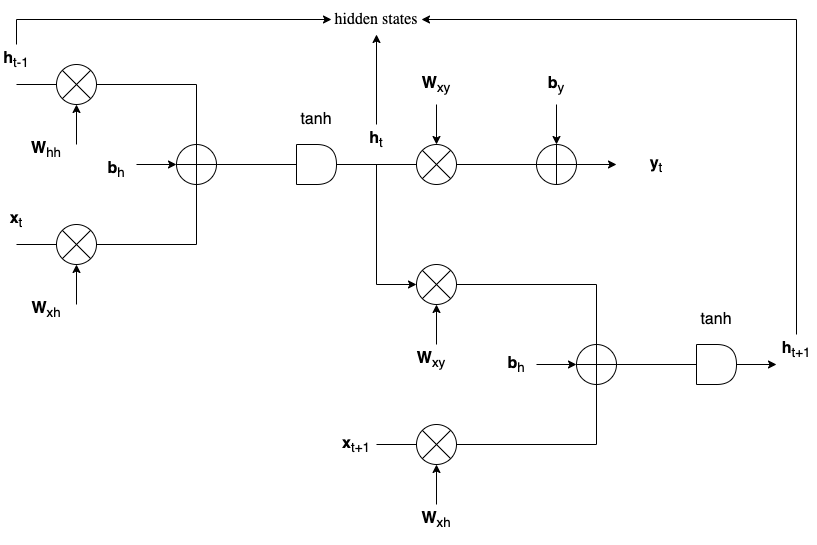
\includegraphics[keepaspectratio,scale=0.5]{chapter2_images/rnn_computational_graph.png}
\caption{Computational graph of a RNN (adapted from \citet{DBLP:journals/corr/abs-1808-03314})}
\label{RNN_architecture}
\end{figure*}

This schema is responsible for introducing the concept of "memory" to RNNs. Note that this feedback loop can be "unrolled" to evidence the network dependence on previous inputs (considering different timestamps for instance) and hidden state values. For computing convenience, in order to perform backpropagation, we must limit some depth to this unroll procedure, propagating the gradients from the last output from the unrolled graph backwards. Following this procedure, the resulting unrolled network turns analogous to a simple feedforward layer network, easing the related computing procedures.

The order-dependence property of a RNN is an extremelly desired characteristic for processing word embeddings, as previously discussed in Section \ref{neural_embedding}, since the neighbouring words often affect or contribute to the meaning representation of a word in a sentence.

\subsection{The first RNN-based machine translator}
\label{learning_phrase_representations}

According to the Cho et al's approach, one RNN sequentially processes each symbol of a sequence of inputs represented by vectors $\mathbf{x}_t$, that represent symbols (typically word or token embeddings), $t \in \mathbb{N}$, encoding into a fixed-length vector representation defined by the encoder hidden state. The equation that abstracts the encoder hidden state computation at a given timestamp $t$ is

\begin{equation}
\label{rnn_hidden_state_eq}
\mathbf{h}^{e}_{t} = f(\mathbf{x}_{t}, \mathbf{h}^{e}_{t-1}),
\end{equation}
where $f$ represents some nonlinear mapping function implemented by the RNN. For a variable-length sequence with size $T_{\mathcal{x}}$ defined by $\mathcal{S}=\{\mathbf{x}_1, \cdots ,\mathbf{x}_{T_{x}}\}$, the information delivered by the encoder to the decoder corresponds to the last hidden state obtained with the Eq. \ref{rnn_hidden_state_eq}, which in turn is called as the context vector $\textbf{c}$.

The second RNN has the task of decoding this representation into a sequence of symbols by predicting the next symbol $y_{t}$ given the context vector $\textbf{c}$ plus all the previously predicted words $\{y_{1},\dotsc,y_{t-1}\}$. In other words, it is possible to compute the probability over a given translation $y$, according to the following decomposition of the joint probability associated with $\mathbf{y}$:

\begin{equation}
p(y) = \prod^{T}_{t=1} p(y_{t} | \{y_{1}, \dots, y_{t-1}\}, \textbf{c}),
\end{equation}
where $\mathbf{y}=(\mathbf{y}_{1}, ..., \mathbf{y}_{T_{y}})$ (the whole range of target words) and c is the previously mentioned context vector. The iterative equation for defining the decoder's hidden state at the time $t$ resembles the one from the encoder as follows 

\begin{equation}
h^{d}_{t} = g(y_{t-1}, h^{d}_{t-1}, \textbf{c}),
\end{equation}
with g representing the function implemented by the decoder RNN. Based on $\mathbf{h}^{d}_{t}$, the $t$-th translated word is calculated using

\begin{equation}
y_{t} = softmax(f(\mathbf{h}^{d}_{t})),
\end{equation}

where $f$ represents one or more feedforward network layers. These equations provide a holistic view of the first encoder-decoder RNN-based translator. In this setup, the encoder and the decoder are jointly trained targeting to maximize the conditional log-likelihood of a target word given a sequence of words from some source sentence and the previous translated words. 

The drawback of this architecture is that some of the information available at the encoder RNN is lost, since only the last hidden state is used, while other hidden state values are discarded. Another issue relates to the fact that the encoder has to compress all the relevant sentence source information into a fixed-length vector. This increases the challenge of dealing with long sentences, which is already complex for any RNN neuron due to the effect of vanishing gradients \cite{DBLP:journals/corr/abs-1808-03314}.

\section{NMT by jointly learning to align and translate}
\label{align_and_translate}

To address the fixed-length and "information compression loss" issues identified in the previous implementation, the authors of the first paper proposed another architecture that changes how the encoder is connected to the decoder in \citet{bahdanau2016neural}. Now, the context vector provided by the encoder to the decoder is multiplied by a weighted "attention" function and integrates multiple hidden-states, not just the last one, defining a variable-length context vector such that $\textbf{c}=\{h^{e}_{1},\dotsc,h^{e}_{T_{x}}\}$. 

In the following sections, we will briefly discuss features and issues that comprises the main contribution of this paper: the attention mechanism. First, this process will be described by high-level illustrated steps to help the reader in grasping the intuition. Then, in the sequence, we will define equations related to them.

\subsection{Some intuition behind the attention mechanism}

Rougthly, the attention mechanism simply assigns weights to words embeddings, allowing a straightfoward implementation of the alignment model presented in Section \ref{word_alignment}. Essentially, these weights define how much attention must the decoder pay for a specific word from the encoder sequence when guessing the next word of the translated sentence. 

Consider the translation of the Portuguese sentence "Vou às dez." to English. In Figure \ref{attention_first_steps} at the step 1, the rectangles that resemble a traffic light represent the RNN neuron at a given sentence iteration, where the circles represent the components of the hidden state vector (see \ref{RNN_architecture} to remind them). Note that each neuron is fed with the hidden state from the previous iteration plus the current input. The attention scores are computed by the dot product between the the embedding associated with the token \textit{Start-Of-Sequence} ("SOS") (written as "$<$sos$>$"), that must be fed at the inputs of the decoder for starting the generation of the translated sequence, and the input sentence. This defines a particular weight for each part of the encoder sequence to compose the context vector used by the decoder with it's current input, to access the next word in the translated sequence. Naturally, the attention weights are recalculated at every step of the translation process, i.e., it is repeated for every next token generated in the output or translated sequence. For computing the attention scores, a softmax layer is commonly used, as discussed further later, and the weights attributed by it are represented by the green bars on the top right of Figure \ref{attention_first_steps} at step 2.

\begin{figure*}[!htp]
\centering 
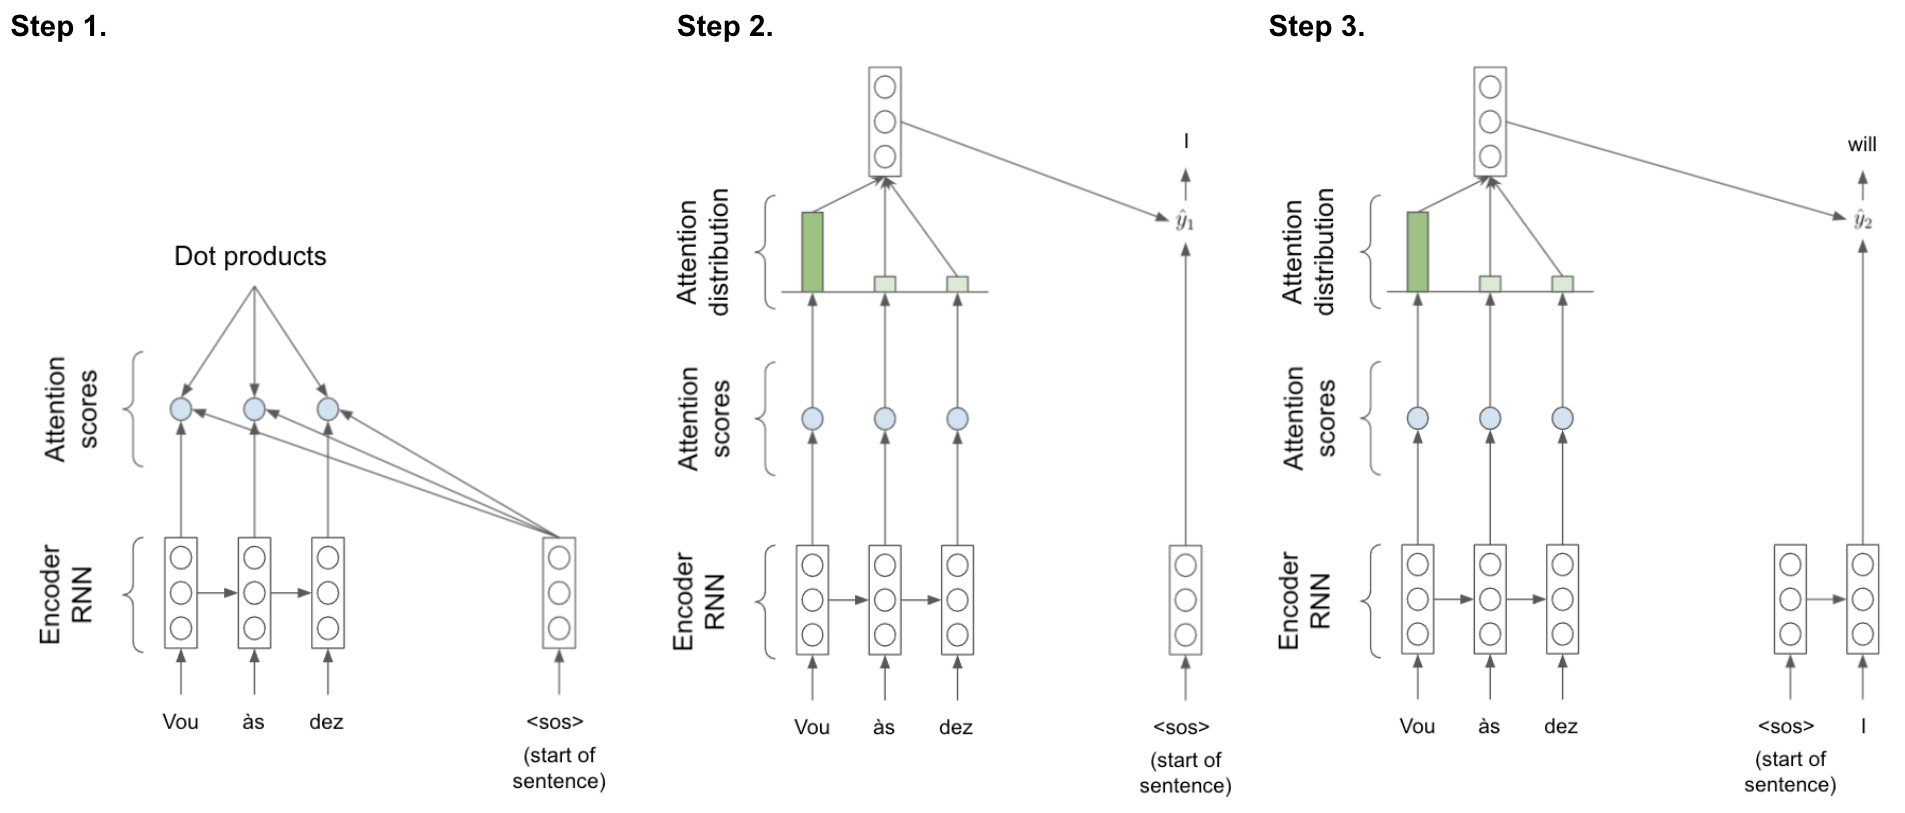
\includegraphics[keepaspectratio,scale=0.223]{chapter3_and_4_images/attention_first_3_steps.png}
\caption{The first steps of how the attention mechanism acts when translating a sentence (adapted from \citet{cs224n_stanford_l7})}
\label{attention_first_steps}
\end{figure*}

Since the model has already been trained on a supervised dataset, it presumedly knows that the word "Vou" must be translated to one or a given set of words in English. In this particular case, when starting from the token "$<$sos$>$", the subject of the verb in Portuguese is hidden, and the subject of the verb is represented by the subjective personal pronoun "I". 

The translation task then keeps producing the the next words based on the input, generating the word "will" after "I" to complement the meaning of the original word "Vou" at step 3. The goal is to match the meaning of an action that will happen at the mentioned time. 

Note that the attention weight distribution changes for each new step. In Figure \ref{attention_last_steps} at step 4, the decoder has already generated the sentence fragment "I will go", corresponding to the original "Vou". Thus, the embedding associated with the token/word "às" becomes the focus, with meaningful attention weight assigned to "dez" as well. 
 
\begin{figure*}[!htp]
\centering 
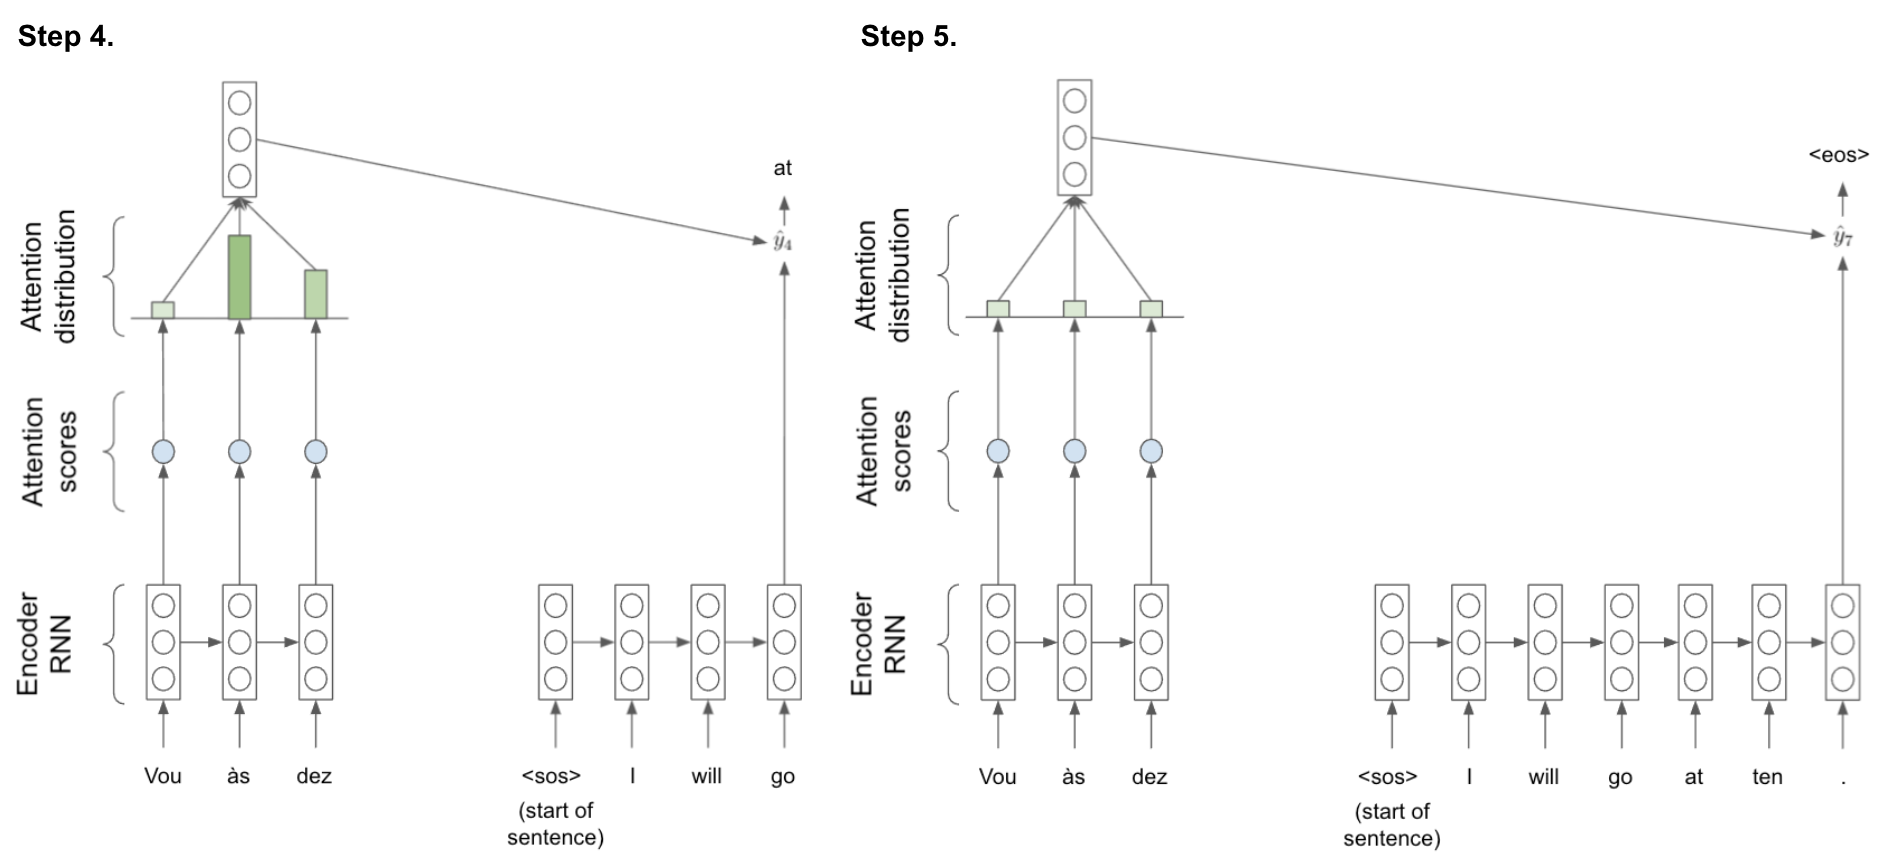
\includegraphics[keepaspectratio,scale=0.223]{chapter3_and_4_images/attention_last_2_steps.png}
\caption{The last 2 steps of attention during the translation of a sentence, adapted from \citet{cs224n_stanford_l7}}
\label{attention_last_steps}
\end{figure*}

In step 5, the other words or tokens related to "ten" and "." are skipped to illustrate how the algorithm ends. When the weights are considered to be low in absolute value with respect to the inputs, it may be a signal that the algorithm has converged. The translation process ends when the $<$eos$>$ token is produced. 

Now that the dynamics of the attention mechanism during the translation is clear, a mathematical walkthrough on the attention layer will be performed.

\subsection{Attention: Calculus background}

Consider the new variable-length context vector defined by a linear combination of several hidden states of the encoder, in opposition to only the last one from the first RNN-based translator model. Now, the context vector will vary according to every input token from the encoder. Let us interpret such words as a set of annotations $\{h^{e}_{1},\dotsc,h^{e}_{T_{x}}\}$. The context vector after applying attention will be computed by a weighted sum of such annotations $h^{e}_{i}$ at a given time $i$:

\begin{equation}
\mathbf{c}_{i}=\sum^{T_{x}}_{j=1}\alpha_{ij}\mathbf{h}^{e}_{j},
\end{equation}
where the variables $\alpha_{ij} \ge 0$ (or attention weights) comprise a mechanism that can be interpreted as how relevant each annotation is from input sentence is when composing $\mathbf{c}_{i}$ for a given token currently processed at the decoder. Such weights are also known as attention coefficients, and represent the probability that a target token $y_{i}$ is aligned to, or translated from, a source token $x_{j}$. These weights shed a light on how the model is aligning and relating words between source and target language, helping to address the challenge stated at Section \ref{word_alignment}. The attention coefficients can be computed in many forms but a common approach is the following

% \textcolor{red}{a explicação para $h_{i-1}$ e nao $h_{i}$ está no paper}
\begin{equation}
\alpha_{ij}=\frac{\exp{(a(h^{d}_{i-1}, h^{e}_{j}))}}{\sum^{T_{x}}_{k=1}\exp{(a(h^{d}_{i-1}, h^{e}_{k}))}},
\label{attention_weights}
\end{equation}
where $a$ is an alignment model that relates the embeddings $\mathbf{h}_{j}^{e}$ in the position $j$ with the embeddings of $\mathbf{h}_{i}^{d}$ at the position $i$. The variable $k$ iterates over the entire range of the input sentence $T_{x}$. The alignment scores can also be interpreted as a way to distribute attention over the input, and $a$ is often parameterized by a feedforward neural network jointly trained with the encoder and decoder parts. The authors also stressed that the attention mechanism relieves the encoder from the burden of having to encode all the information from the source sentence, hence contributing to the resilience of this approach when dealing with long sentences.

Another improvement in this work that contributed to the success of this approach is the use of bidirectional RNNs to encode the input sequence. The key difference from this to the unidirectional RNN is that the context vector now aggregates information relative to the representation not only of the preceding words but also from the following words, allowing a more efficient attention weight distribution. This vector is simply defined by a concatenation of the representations obtained from the forward and the backward RNN hidden states. Despite these improvements, the attention mechanism is still rather simple, since it is based only on a additive attention, while later variants compose additive with multiplicative attention and even types of distributions \cite{luong-etal-2015-effective}. Due to this gap, the importance attribution isn't performed as well as it is in the succeeding variants, implemented in other papers later on.

Another detail that contributed to model performance despite not clearly highlighted in the paper (only mentioned) is the use of a beam search decoding algorithm. This algorithm was first proposed as a generic sequence transducer \cite{DBLP:journals/corr/abs-1211-3711}, but only a few years later was exploited in MT \cite{DBLP:journals/corr/SutskeverVL14}. The main benefit it brought results in a more efficient and accurate search of the most probable next word given a set of preceding words. It reduces the chance of the algorithm to get trapped in local optimal solutions compared to the Greedy Search algorithm, thus allowing the NMT model to explore more translation variants and converging to more realistic translations. 

\subsection{Search algorithms for NMT}

After converging to a local optimum and learning word vector representations that reflect semantical and syntactical attributes of the words, the model can be tested and generate translations. When accomplishing the task of generating translations, the quality of the search performed and number of possibilities considered by the algorithm make a difference on the final result. The traditional approach and a more clever one will be discussed here: the greedy search and the beam search, respectively.

\subsubsection{Greedy search}

This was the approach used for the first RNN-based translator described in Section \ref{learning_phrase_representations}. It is considered as the simplest way to generate a translation given the context, as it predicts the most likely word by considering a given set of previous words. This rather simple search is used since the beginning of the field of statistical Machine Translation. The goal is to obtain the next $\hat{y}_{t}$ iteratively such that

\begin{equation}
\hat{y}_{t} = argmax_{y_{t}}P(x_{t}|y_{t-1})P(y_{t-1}),
\end{equation}
in each timestep $t$ the probability of the next word is calculated, considering $x_{t}$ as the representation of a sentence in the source language and $y_{t-1}$ is the current composition of the target sentence built at the timestamp $t$. This algorithm has the drawback of being impossible to go back after generating an unnatural or sub-optimal sentence. Basically, a token that looks good to the decoder at a given moment might turn out later to have been a wrong choice. When this happens, the model gets limited to generating new words on top of the current sub-optimal sentence, hence the translation loses fluency. Nonetheless, it was the top of mind algorithm for the MT community for a long time.

Ideally, the only method that guarantees to find the best translation is the exhaustive search. Given a vocabulary with size $V$, the exhaustive search would be performed by computing and evaluating each one of the $V^{T}$ word combinations, with $T$ being the length of the translation in words. Going over such a large word search is obviously too expensive. Hopefully, a more cost-effective search variant that considers more words than the greedy variant and that is less complex than the exhaustive one was created. 

\subsubsection{Beam Search}

In this algorithm, instead of choosing the best token at each timestep, $k$ possible tokens are kept at each step. This fixed-size parameter is called the beam width. It works by assigning a probability to the generation of each word in the current translated sequence, for each of the $k$ available candidates, wherein this probability is obtained through a softmax calculated over the entire vocabulary. These numbers are then sorted from the most probable to the least, and only the $k$ best possible tokens are retained for the succeeding step. Such candidate tokens are called hypotheses, and this process of calculating probabilities, sorting the sentences and progressively adding words at the end of the sentence at each step means that the algorithm is simultaneously evaluating a set of $k$ different sentences.

\begin{figure*}[tb]
\centering 
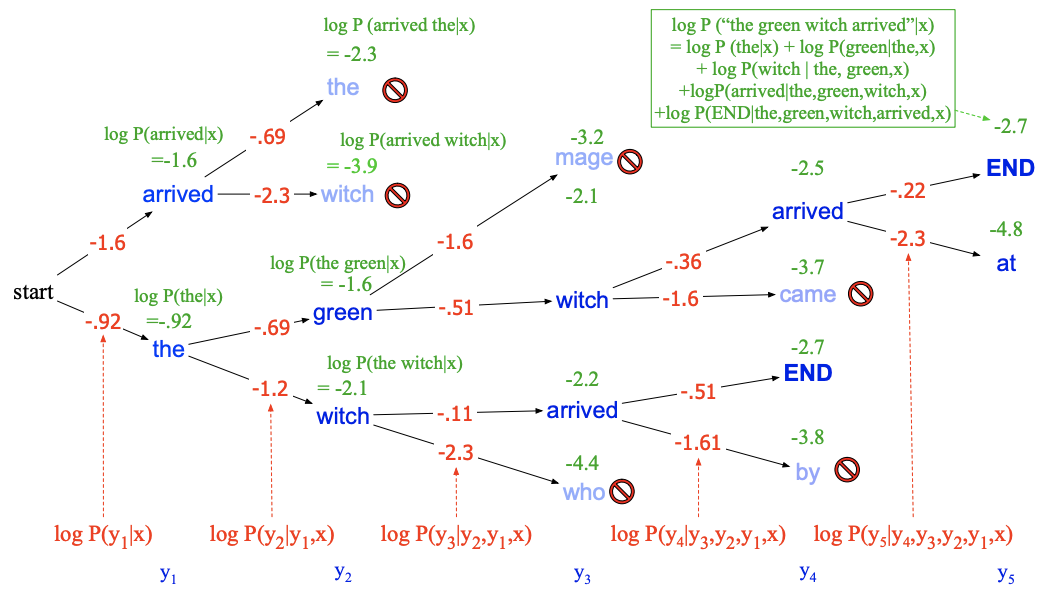
\includegraphics[keepaspectratio,scale=0.7]{chapter3_and_4_images/beam_search.png}
\caption{Example of beam search with beam width of size 2, taken from \citet{nmt_nlp_speech_draft_book}}
\label{beam_search}
\end{figure*}

A hypothesis only stops being evaluated if it ends with an $<$eos$>$ token, or if it is not within the top $k$ options. If an $<eos>$ token is reached, the sentence is placed aside and other hypothesis continue to be explored. This process is repeated until all the hypothesis reach an $<eos>$ token or the maximum predetermined sentence length (in words). Figure \ref{beam_search} shows an example for a small sentence using beam width of size 2, where "arrived" and "the" are the first guesses, later producing 4 words where only the 2 most probable were selected. After picking "green" and "witch" by sorting probabilities in a descending order, another 4 words are generated, and the process is repeated until convergence.

Besides the practical gains regarding fluency, this algorithm has the drawback of penalizing longer sentences with lower scores. Moreover, this issue can be partially addressed by a length normalization factor, but not totally mitigated. Beam search has become the standard approach in NMT, with a good starting point being the use of a beam width of size 3, the same adopted in our experiments.

\subsection{Exploring RNN-based sequence to sequence architectures}

An interesting work that illustrates the potential of the previously presented RNN models is due to \citet{britz2017massive}. They use \cite{cho-etal-2014-learning} as a base model and evaluated the tuning of several hyperparameters, like embedding size, RNN cell variant (LSTM and GRU), encoder and decoder depth, unidirectional vs. bidirectional RNN encoders, attention mechanism and beam width parameters. One of the claims of this work is that careful hyperparameter tuning can yield better results than exploring architecture variations.

Here are some interesting findings reported by \citet{britz2017massive}: (1) larger embeddings consistently outperforms smaller ones by a thin margin, (2) LSTM cells consistently outperformes GRU cells, (3) deeper decoders tend to lead to performance increases, (4) additive attention achieves slightly better results than multiplicative attention and (5) beam searches tuned to a "sweet spot" can increase the model performance up to 5\%.

\section{Transformer models}

\begin{figure*}[tb]
\centering 
\includegraphics[keepaspectratio,scale=0.7]{chapter3_and_4_images/Transformer_architecture.png}
\caption{Transformer model architecture, taken from the original paper \cite{DBLP:journals/corr/VaswaniSPUJGKP17}}
\label{Transformer_architecture}
\end{figure*}

One contribution switched the focus on recurrent and convolution-based neural network models for NMT in 2017: the Transformer architecture. Introduced in the seminal work of \citet{DBLP:journals/corr/VaswaniSPUJGKP17}, this model is not subjected to the same issues faced with RNNs. Due to their sequential processing structure, RNNs have to wait for an internal operation to finish before beginning with another one, which isn't the case of Transformers. This new approach gained traction and adherence from the community, since its massive parallelization is one of its major strengths.

In the original implementation, the encoder and the decoder exploit 6 stacked Transformer layers. Regarding the encoder, each layer contains a multi-head self-attention mechanism, followed by a layer normalization and a position-wise feedforward fully connected layer, represented by the "Add \& Norm" block depicted in Figure \ref{Transformer_architecture}. A residual connection is also employed around each of the 2 blocks inside a Transformer layer, represented by the arrow that goes into the "Add \& Norm" blocks. The structure of the decoder is quite similar, differing by the existence of an extra masked multi-head attention layer added over the output of the encoder stack, before the multi-head attention block. This mask, combined with an offset in the target sentence (output embedding) by one position, ensures that the predictions for a given position $i$ depend solely on the known inputs for positions less than $i$. Backpropagation operates end-to-end for training this architecture.

\subsection{Unveiling self-attention}

The attention mechanism adopted here differs from previous implementations, but the overall goal is the same: enabling the model to distribute the influences of every input word on the output words generated. Consider a scenario where there are a set of $i$ feature vectors available, which we call values $\mathbf{V} \in \mathbb{R}^{i \times j}$. The model can dynamically map a feature vector to a key, based on how similar the input query vector $\mathbf{q} \in \mathbb{R}^{q}$ is to a set of $k$ keys $\mathbf{K} \in \mathbb{R}^{i \times k}$. The mapping is performed depending on the similarity of the input with the query, hence if $\mathbf{q}$ is most similar to $\mathbf{k}_{i}$ and has some similarity with $\mathbf{k}_{i+1}$, but is uncorrelated with the rest, the values $v_{i}$ and $v_{i+1}$ are used in a weighted sum with $v_{i}$ having the strongest weight \cite{pml1murphy}. 

The query ($\mathbf{Q}$), keys ($\mathbf{K}$) and values ($\mathbf{V}$) are all matrices with dimensions defined by the respective hyperparameters, set to 64 in the original work. Attention's "keys and values" correspond to hidden state representations learned by the sequence to sequence networks \cite{eisenstein2019introduction}, and "queries" will be input token embeddings or intermediary representations of them provided by the Transformer layers. 

The core of this new mechanism is still pretty much the same as the one used by \citet{bahdanau2016neural}. The attention weights are defined by a similar equation to Eq. \ref{attention_weights}, whereas they are now given by Eq. \ref{selt_attention_weights}:

\begin{equation}
\alpha_{ij} = \frac{\exp{(e_{ij})}}{\sum_{i'} \exp{(e_{i^{'}j})}}
\label{selt_attention_weights}
\end{equation}
where 
\begin{equation}
e_{ij} = \mathbf{Q}^{T}_{j}\mathbf{K}_{i}.
\label{key_query_affinity}
\end{equation}

% http://web.stanford.edu/class/cs224n/slides/cs224n-2021-lecture09-Transformers.pdf

In such equations, $\mathbf{Q}$ and $\mathbf{K}$ are representations for the queries and keys matrices respectively and $i$ and $j$ represent positions in the input and output. The equivalent weighted sum that produces the output of the self-attention layer $\mathbf{y}$ for Transformers also shares similarities with RNNs:

\begin{equation}
\mathbf{y}_{j} = \sum_{i}\alpha_{ij}\mathbf{V}_{i}.
\label{Transformer_output}
\end{equation}

\subsubsection{Scaled dot-product attention}

The name scaled dot-product attention comes from the strategy of normalizing the dot products between the query matrix and the key matrix entries, normalized (scaled) by $\sqrt{d_{k}}$, before submitting them to a softmax layer to produce the weight factors that will linearly combine the vectors stored in $\mathbf{V}$. The result of this operation are the weights for the correspondent values. This mechanism is illustrated in Figure \ref{scaled_dot_prod_attention}, where MatMul represents a matrix multiplication block and the mask is optional, used only in the decoder. Mathematically speaking, we have

\begin{equation}
Attention(Q, K, V) = softmax(\frac{QK^{T}}{\sqrt{d_{k}}})V.
\label{attention_equation}
\end{equation}

One of the major advantages from dot-product attention is that it is space-efficient. It can be implemented using optimized matrix multiplications; thus, benefitting from parallel architectures as compared to additive attention, for instance. The scaling factor is a plus from the authors to the original dot-product attention, as they claim that it helps in reducing the magnitude of the dot-products, which may push the softmax function to flat regions, wherein the associated gradients may be small. 

\begin{figure*}[!htp]
\centering 
\includegraphics[keepaspectratio,scale=0.25]{chapter3_and_4_images/scaled_dot_prod_attention.png}
\caption{Illustration of the Scaled Dot-Product Attention mechanism, taken from \citet{DBLP:journals/corr/VaswaniSPUJGKP17}}
\label{scaled_dot_prod_attention}
\end{figure*}

\subsubsection{Multi-head attention}

% Due to training converging issues, since the dimensionality of the vectors stored in the matrices Q an V is typically high (often between 512 and 1024), it is convenient to split this attention block into several smaller block involving smaller submatrices produced by linear projections of Q, K and V, and after concatenate the representations produced by each one.

Essentially, this technique performs the concatenation of scaled dot-product attention blocks. The assumption behind it is that different learned projections of the same $\mathbf{Q}$, $\mathbf{K}$, $\mathbf{V}$ matrices yield representations that may complement each other, as an ensemble of attention heads, delivering distinct features of the same data. Figure \ref{multi_head_attention} illustrates this trick. One may readily note that the result of the concatenated matrices goes through a linear feedforward layer on the top.

Multi-head self-attention also plays a major role on the overall performance of the Transformer. The authors claim that it is beneficial to project the matrices $\mathbf{Q}$, $\mathbf{K}$ and $\mathbf{V}$ in attention $h$ times, where $h$ is the number of attention heads, thus exploiting different learned projections. The attention weights are adjusted to such different representation subspaces depending on the query and available keys. The original paper uses $h=8$ heads. An usual recommendation that should be followed in this case is that the original hidden size $d_{model}$ must be divisible by the number of attention heads. 

\begin{figure*}[!htp]
\centering 
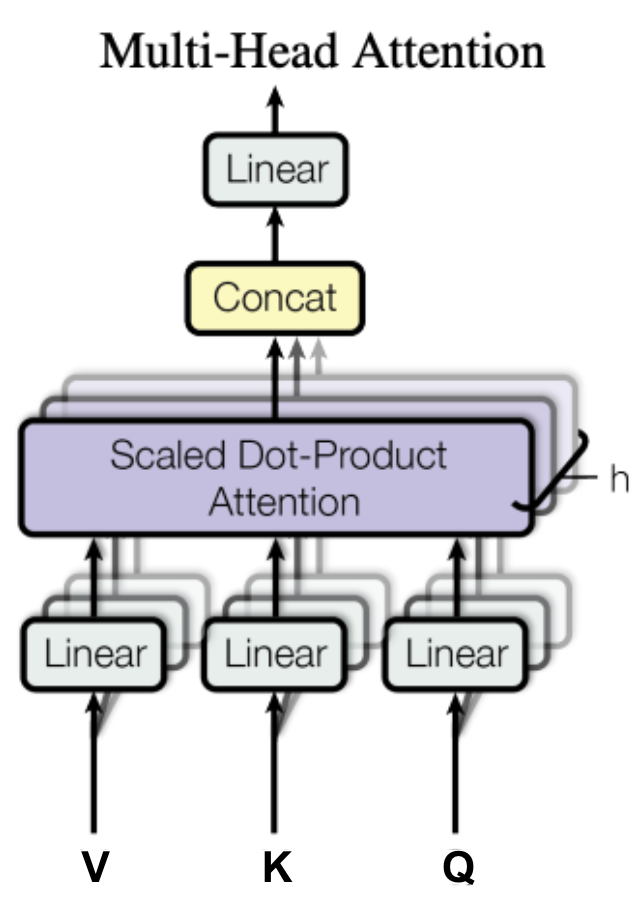
\includegraphics[keepaspectratio,scale=0.25]{chapter3_and_4_images/multi_head_self_attention.png}
\caption{Illustration of the Multi Head Attention mechanism, taken from \citet{DBLP:journals/corr/VaswaniSPUJGKP17}}
\label{multi_head_attention}
\end{figure*}

At the time of the original paper writing, multi-head self-attention was thought to be consistently contributing to the Transformer performance. Years later, after an analysis performed by \citet{DBLP:journals/corr/abs-1905-09418}, this hypothesis was rejected. The authors evaluated how each attention head contributes to the solution of a translation task, and find out that only a small subset of the heads would be enough to sustain the Transformer translation scores. Their analysis was based on the importance distribution, a heatmap that correlates each output word with every input word, discovering that several heads have learned similar dependency mappings. By using this map as a qualitative indicator of the feature importance of each head, they pruned the heads with similar dependency maps, concluding that there is no noticeable loss in the translation quality in this case.

This paper also raised a relevant question to the community: are deep learning models usually biased towards increasing complexity and model parameters unnecessarily? Less complex models have a smaller carbon footprint and energy waste, which can lower their impact on the nature, bringing the NMT community closer to the status of Green AI.

\section{Attention variants for sequence to sequence learning}

Not only architectural improvements can lead the Transformers to translations of high quality, the attention mechanism has also received some relevant contributions. In the approach followed by \citet{DBLP:journals/corr/abs-2006-10270}, the multi-head attention is modified to a new mechanism called multi-branch attention, where each branch is an independent multi-head attention mechanism. 

Despite the evidence that increasing the number of attention heads may lead to redundancy, this work outperformed the standard Transformer baseline, which goes against the analysis previously stated. In this paper, other techniques such as a drop branch mechanism (similar to Dropout \cite{JMLR:v15:srivastava14a}, but applied to the Transformer's branches) and a specific initialization recipe for each branch may have impacted the final outcome. The composition of such techniques makes unclear whether the benefits come from scaling the attention complexity or from those architectural alternatives.

Going back to the literature, variants applied over the set of words that the attention blocks sees and over the weight distribution functions are among the most common variants explored. In the paper published by \citet{luong-etal-2015-effective}, the attention mechanism is split into 2 classes: global and local attention. The former always attends to all source words of a given sentence, while the latter only looks at a subset of words at a given time. 

Local attention is explored with different alignments: monotonic and predictive. In the first case, they just assume that the source and the target sequences are roughly monotonically aligned, and concatenate the target hidden state $\mathbf{h}_{t}$ with the equivalent source version $\mathbf{h}_{s}$. In the predictive variant, they use a Gaussian distribution centered around the word to be predicted and define alignment weights based on the values of the gaussian, so nearby words are more important than distant words. Following this approach, the attention weights are biased to follow a normal distribution.

The main findings of this paper are: (1) attention-based models usually outperform non-attentional ones and (2) properly tuning the alignment model can yield to better results. A small increase in the performance was observed by adding a custom weight function (Gaussian-based in this case). They also concluded that using an ensemble involving some of the proposed attention architectures may be effective. However, further details of how this ensemble was implemented are not provided.

Incorporating different attention perspectives to the attention mechanisms with is another common exploited approach, which has been followed by \citet{calixto-etal-2017-doubly} and \citet{cui-etal-2019-mixed}. In \cite{calixto-etal-2017-doubly}, a single layer feedforward network is used to compute the expected alignment between each annotation vector in both mechanisms, but this increases the amount of parameters to be trained on the model. In \cite{cui-etal-2019-mixed}, the concept of forward and backward attention is introduced, where specialized masks help the Transformer to model word order information, a slightly different schema than the positional encoder used in the original paper. Both mechanisms are concatenated with the standard global and local attention. Even though this approach leads to a better BLEU score, it also increases the number of model parameters.

There is no strong evidence that tuning the attention mechanism would provide relevant benefits in low-resource settings. Furthermore, all variations usually increase the quantity of model parameters, raising its complexity and amount of data required for learning, along with the amount of resources required to be trained (GPU memory). In a single GPU scenario, a larger and more robust GPU would be necessary in these cases. Increasing the number of GPUs unfortunately does not fit in the scope and budget of this work. However, data augmentation and embedding techniques have a higher potential to succeed in low-resource settings, hence the focus of this work was shifted away from a possible tuning of attention mechanisms.

\subsection{Positional encoding}

To insert information relative to the order of words in a sequence without recurrence or convolutions, the encoder augments the base layer of the network with positional encodings correspondent to the ordered occurrence of each word in the source sentence. Considering for instance a sequence length of $n=5$ and the use of 3-dimensional bit vectors to represent each word $d=3$, we could generate vectors to represent the location of words like $\mathbf{l} \in {000, 001, ... 110, 111}$. The position matrix can be represented by $\mathbf{P} \in \mathbb{R}^{n \times d}$ A more compact representation of word position based on these location vectors can be obtained by using basis functions and real-valued weights. \citet{DBLP:journals/corr/VaswaniSPUJGKP17} proposes a sinusoidal basis to encode position:

\begin{equation}
\mathbf{p}_{(i, 2d)} = \sin{(\frac{i}{C^{\frac{2d}{d_{model}}}})},
\end{equation}
and
\begin{equation}
\mathbf{p}_{(i, 2d + 1)} = \cos{(\frac{i}{C^{\frac{2d}{d_{model}}}})},
\end{equation}
where $d$ is the dimension or level within the representation (the amount of real numbers used to represent a word) and $C$ corresponds to a maximum sequence length, set to $10000$ in the original paper. If a hypothetical matrix has dimensions $n \times 4$, then it's $i$th row is given by

\begin{equation}
p_{i} = [\sin{\frac{i}{C^{\frac{0}{4}}}}, \cos{\frac{i}{C^{\frac{0}{4}}}}, \sin{\frac{i}{C^{\frac{2}{4}}}}, \cos{\frac{i}{C^{\frac{2}{4}}}}].
\end{equation}

Figure \ref{positional_encoding_illustration} provides a more intuitive view of how the absolute values of a matrix $\mathbf{P} \in \mathbb{R}^{n \times d}$ representing a sequence of length $n=60$ and and an embedding dimension of size $d=32$ contribute in encoding the word position.

\begin{figure*}[!htp]
\centering 
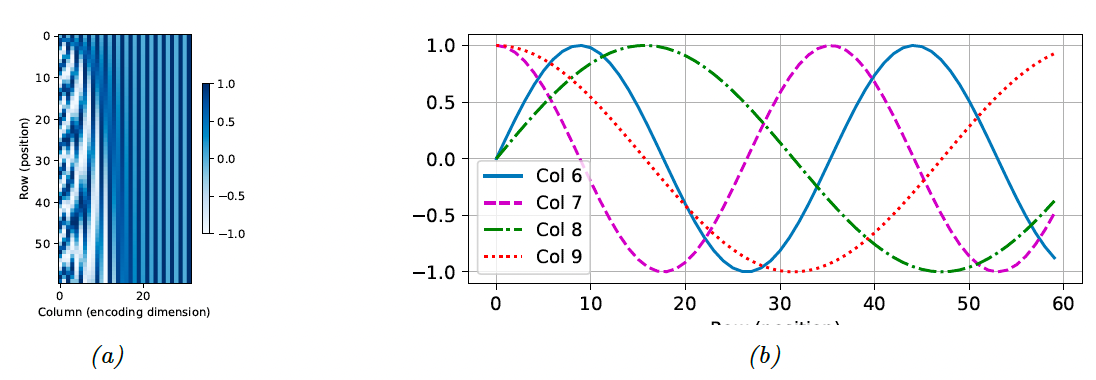
\includegraphics[keepaspectratio,scale=0.3]{chapter3_and_4_images/positional_encoding_illustration.png}
\caption{(a) Positional encoding matrix with dimensions $n=60$ and $d=32$. (b) Basis functions for columns 6 to 9. Generated by \url{http://code.probml.ai/book1/15.25} and adapted from \citet{pml1murphy}.}
\label{positional_encoding_illustration}
\end{figure*}

This representation brings a two-fold advantage: first, it can be computed for arbitrary length inputs (up to $L \leq C$), unlike the common mapping from ids to words approach \cite{pml1murphy}. Second, the representation of one location is linearly predictable from any other, given the knowledge of their relative distance \cite{pml1murphy}. Any word position can be modelled by $p_{t+\phi} = f(p_{t})$, where $f$ is a linear transformation, and this property is inherited due to the use of trigonometric functions. Note this by the following decomposition

\begin{equation}
     \begin{bmatrix}
     \sin{(\omega_{k}(t + \phi))} \\
     \cos{(\omega_{k}(t + \phi))}
     \end{bmatrix}
     =
     \begin{bmatrix}
     \cos{(\omega_{k}\phi)} & \sin{(\omega_{k}\phi)} \\
     -\sin{(\omega_{k}\phi)} & \cos{(\omega_{k}\phi)}
     \end{bmatrix}
     \begin{bmatrix}
     \sin{(\omega_{k}t)} \\
     \cos{(\omega_{k}t)}
     \end{bmatrix}.
\end{equation}

If $\phi$ is small, then $p_{t+\phi} \approx p_{t}$, correctly inducing the desired relative position correlation. Once the positional encodings $\mathbf{P}$ are computed, they are combined with the original word embeddings $\mathbf{X}$ through the following:

\begin{equation}
POS(Embed(\mathbf{X})) = \mathbf{X} + \mathbf{P}.
\end{equation}

\section{Relevant Transformer variations}

Since their publication, Transformers were customized in many ways by researchers aiming to define new state of the arts. Not all the variations are worth a story to tell, but some of them have exceeded expectations and deserve some space in this discussion. Beginning with BERT (Bidirectional Encoder Representations from Transformers)\abbrev{Bidirectional Encoder Representations from Transformers}{BERT}, the Transformer idealized by \citet{DBLP:journals/corr/abs-1810-04805}, designed to extract deep bidirectional representations from unlabeled text.

Roughtly, two interesting tasks can be addressed with BERT: one is predicting masked tokens in a sentence, i.e., the BERT performs like a masked language model. In this case, during training some percentage of the input tokens are hidden at random, and the tokens masked are predicted by the model. The second aims to extend the model's functionalities to other NLP tasks, such as question answering and natural language inference, and this is accomplished via next sentence prediction. The intriguing aspect of BERT is that it can be easily fine-tuned to perform a wide range of tasks, while still keeping an architecture that isn't far from the original Transformer. In these cases, this model still beats the best results available for a range of tasks, such as natural language understanding, inference and question answering.

Some other variants of the traditional Transformer architecture were heavily focused on increasing complexity aiming to surpass the state of the art, and solving a wider number of tasks. The variant presented by \citet{brown2020language} have shown that it is possible to improve the performance of the model by simply increasing the model size, and, as a consequence, the dataset size and the computational power used as well. 

A typical example is the GPT-3. This model comes in various sizes, with the smallest model having 125M parameters, 12 attention layers, each one with 12 heads of dimension 64. The largest version has 175B parameters, along with 96 attention layers, each one containing 96 heads with dimension 128. This model has raised an environmental concern, as it spent about 190,000 kWh to be trained \cite{quach_2020}. Some GPT-3 outcomes are interesting to highlight: (1) in text generation, humans have failed in discriminating artificially generated summaries from genuinely human-made texts for 24\% of the cases, (2) Machine Translation, surpassing the best available BLEU scores with many language pairs where the English idiom figures as target and (3) other less traditional tasks, such as arithmetic and word scrambling. 

Not all the Transformer variants focused on firepower, though. There is some research aiming to come up with lightweight alternatives to the Transformer. In this case, the main goal is increasing the model performance but still keeping the computational burden under satisfactory standards. Both models proposed on \citet{DBLP:journals/corr/abs-1911-12385} and a year later on \citet{mehta2021delight} are able to improve the efficiency of the original Transformer as a language model on a range of tasks. The definition of efficiency here is achieving a high BLEU score (for NMT) or another score (for other tasks), considering the number of model parameters integrating the cost function.

The Delight model, one of their most recent works, have changed the inner mechanism of the Transformer layer by using the delight transformation, which is composed by a group of linear transformation layers that are shallower and narrower near the input while deeper and wider near the output. The authors state that this transformation decouples attention dimensions from the depth and width, allowing representations to be learned efficiently using block-wise scaling. Delight also replaces the multi-head attention mechanism for single-head attention, reducing the number of parameters needed in trainiing. Over the WikiText-103 dataset, the authors obtained an increase on BLEU score of 3.3\%, while using only 80\% of the standard Transformer parameters and requiring just 23 hours to train, as opposed to the 37 hours used by the original model.

\section{Alternative training objectives}

Many of the state-of-the-art models have reached their related scores using the traditional cross-entropy loss. Most language models have also focused on maximum likelihood learning objective, as stated in \citet{DBLP:journals/corr/abs-2012-15515}. This work focused on reviewing the main contributions and the tools available for executing the NMT task, pointing out the distinguishing ones that happened through time. 

Let $\mathbf{x}$ be the real-valued representation of a token in the source language and analogously $\mathbf{y}$ the same for a token in the target language. The equation to obtain log-likelihood as per the original model is defined as

\begin{equation}
L(\theta) = \sum^{S}_{s=1} \log{P(y^{(s)}|x^{(s)}; \theta)},
\end{equation}
where $\mathbf{x}$ and $\mathbf{y}$ are pairs of the training set $D=\{(x^{(s)},y^{(s)})\}^{S}_{s=1}$ of size $s$, and $\mathbf{\theta}$ represent the model parameters. The standard goal of most NMT algorithms is maximizing the value of this function on the training set data, as follows

\begin{equation}
\hat{\theta}_{MLE} = argmax(L(\theta)).
\end{equation}

Nevertheless, the work of \citet{ranzato-sequence} indicate two drawbacks of this approach. First, NMT models are usually trained on a specific dataset, but are not exposed to their own translations and consequently their own errors: this phenomenon is referred to as exposure bias. Finally, the MLE estimation is defined at the token-level rather than sentence-level. So, theoretically, the objetive settled by the optimization is not aligned with the final objective, which is generating a sentence that matches a correct human translation.

With this problem in mind, these authors introduced the Mixed Incremental Cross Entropy Reinforce (MIXER), which switches the learning objective towards a sentence-level training. The proposed algorithm tries to handle the problem of backpropagating gradients from non-differentiable metrics like BLEU, exploiting some ideas borrowed from the Reinforcement Learning (RL) area \abbrev{Reinforcement Learning}{RL}. 

Other works have also put efforts in this learning objective issue. For instance, the technique proposed by \citet{shen-etal-2016-minimum}, called Minimum Risk Training (MRT) \abbrev{Minimum Risk Training}{MRT}. In this learning objective, the model considers the discrepancy between its prediction and the equivalent gold standard translation. The model generates multiple samples from the search space provided by beam search to calculate the expected risk, and the risk is defined as the expected loss with respect to the posterior distribution. This loss function is not parameterized, thus, not differentiable, and can also be negative when considering sentence-level evaluation metrics such as BLEU.

The work of \citet{shen-etal-2016-minimum} reported better results than \citet{ranzato-sequence}. The authors' allegation for this is because MIXER samples only one candidate to calculate the reward, while their approach, Minimum Risk Training (MRT) \abbrev{Minimum Risk Training}{MRT}, generates multiple samples. This potentially increases the MRT's discrimination capabilities, pretty close to the effect of increasing the beam size in beam search in a standard NMT setup.

Apart from the efforts put into iterating on the learning objective and the alleged benefits claimed by these papers, some side effects of switching the training objective are also pointed by \citet{DBLP:journals/corr/abs-1907-01752}. A major pointed issue is the weakness of RL-based approaches for optimization, the fact that some gains can not be fully attributed to the techniques, and some convergence issues related to the training objectives proposed by \citet{shen-etal-2016-minimum} and \citet{ranzato-sequence}. Therefore, based on the presented review of the literature, the potential of changing the learning objective to obtain better translations under low-resource is uncertain. As a result, this work opted for not considering changes in the learning objective.

\section{Alternative positional encoding}

The positional encoding performed by the traditional Transformer is called absolute positional encoding. As it simply adds the positional embeddings to the original word embeddings, it comes with the drawback that word position and word meaning are entangled, despite representing unrelated information. The work of \citet{DBLP:journals/corr/abs-2006-15595} warns for the potential to bring mixed correlations between the word semantics and the position information itself, adding unwanted noise to the learning process and limiting the expressiveness of the model.

They propose the use of Transformer with Untied Positional Encoding (TUPE), that computes the
word contextual correlation and positional correlation separately with different parametrizations and then adds them together. By following their approach, the resulting attention weights can be decomposed into terms that represent interactions between word-to-word, word-to-position, position-to-word and
position-to-position, where they claim to enrich the word representation \cite{DBLP:journals/corr/abs-2006-15595}. Their model is compared with other propositions of the literature for positional encoding, like mixing relative positional encoding with absolute positional encoding and obtain superior performance on the GLUE dataset benchmark.

\chapter{The low-resource domain context}
\label{low_res_context}

The term "low-resource" recalls situations where any of the resources needed to perform to one task are scarse. In NMT, this phenomenon can manifest itself in a number of ways. Complex models that contain a high amount of parameters to be learned also demand an abundant quantity of data, a phenomenon that is explained by the VC (Vapnik-Chervonenkis)\abbrev{Vapnik-Chervonenkis}{VC} dimension theory. If a supervised complex model has scarce data for a task and its training process is limited to that data, its potential to achieve relevant generalization scores can be significantly hindered. This can even lead to simpler algorithms outperforming more complex models in a given task. There are some situations to which phrase-based Machine Translation models can surpass neural-based models, especially when the dataset is small, such as the case study reported in \citet{sennrich-zhang-2019-revisiting}.

Scarce data also often strongly contributes to increase the open vocabulary challenge, mentioned in Section \ref{open_vocabulary}. Solving the translation task with reduced data also means solving the open vocabulary challenge under adverse conditions. Increasing the corpus content complexity somewhat increases this challenge, so a technique adopted to solve the issue must be resource efficient to excel under such conditions. 

The second most important issue that is fundamental for the success of a translation model is the infrastructure used for training, which usually needs to involve one or more GPUs or TPUs (Tensor Processing Units)\abbrev{Tensor Processing Unit}{TPU}. Models that require a high batch size such as Transformers cannot be trained in practical terms with a CPU. Switching from CPU to GPU may accelerate the training process hundreds of times, which may correspond to a difference from hours to days for completing the task. 

The memory footprint required by a dataset in some infrastructure is directly related to its size. Two dataset dimensions that directly influence the memory footprint are the number of sentences and number of words per sentence. Such numbers are relevant to determine the ideal batch size. 

Another factor that has an influence on the choice of the batch size is the amount of trainable parameters in a model, which increases linearly with the depth of a neural network. A common practice is to increasing the batch size proportionally to the network depth. This approach may be observed in GPT-3 variants described in the work of \citet{brown2020language}. There is no theory establishing a deterministic rule relative to how the batch size must be increased as a function of the number of parameters. However, it seems to be a good practice to consider them directly proportional, to achieve a better generalization during training.

Other factors must be also considered when one addresses a NMT task, but they rarely represent a bottleneck: disk storage, internet connection and a correctly configured python environment (or another language of choice). They don't usually represent the biggest challenge because such resources are more accessible than cutting edge GPUs. When referring to low-resource domains in the following sections, only the dataset size and the GPU power constraints are considered.

Fortunately, techniques that turn the NMT models more resilient to open vocabulary and some of the previously mentioned issues are available in the literature. Some of these startegoes will be addressed in the following sections, right after a brief overview of a few challenges faced while tackling Portuguese NMT under low-resource settings.

\section{Intrinsic challenges of this work}

Before focusing our studies in low-resource approaches, our initial objective was creating a model to surpass the state of the art. However, as soon as the computational infrastructure at our reach has shown its intrinsic limitations we realized that it wasn't possible to compete with the literature in such a level. To perform experiments involving datasets of different lengths and tuning hyperparameters for Transformer variants can be quite challenging when one uses a 12GB GPU, which is the standard low-cost or free cloud hardware solution in 2021. 

Transformer variants have shown an astonishing performance in a variety of practical applications, attracting multiple companies and dedicated research groups seeking to reach the state-of-the-art status. Researchers from more resourceful countries or universities usually have multiple GPUs in the same cluster, enabling them to evaluate solutions with a higher GPU memory usage. However, this can be quite expensive without sponsorship to get on your own. Given such limitations, our decision was to contribute to the low-resource branch of NMT given the overall practical limitations.

The process of understanding the constraints of our environment (specially GPU memory related) also involved a non-friendly trial-and-error approach. Even when setting our batches to begin higher than usual and dwindle in size, the out of memory error does not usually appear in the beginning of the first epoch or even in the first few epochs. Frequently, we had to conduct a number of experiments that took some time until fail aiming to understand what infrastructure factors are constraining the experiment to happen as desired. This trial-and-error process was repeated whenever the dataset used or the number of parameters (complexity) of the model being trained was changed, significantly increasing the time spent in performing the experiments with different datasets and techniques.

The following sections provide a brief coverage over the techniques considered in this work to deal with low-resource issues and some technical trade-offs necessary to be settled when using them in the NMT context.

\section{Subword embeddings}

In Chapter 2, we only mentioned some interesting aspects of switching to the subword level. In this section, we provide a more detailed explanation of how the subword models operate. The process is quite similar to producing vector embeddings for the words in a sentence (word embedding), differing in the sense that each word is broken into several tokens, and to each token is produced an embedding vector. The methodology that dictates how words are split into subparts has an important influence in the explainability (quality) of the final subword representations.

This type of embedding is more robust relatively to the out of vocabulary (OOV) occurrence as compared to the traditional word-level approach \cite{eisenstein2019introduction}. When one breaks a word into smaller tokens, the smaller resulting tokens are often more likely to appear in both training and test sets. Considering the translation of rare tokens, the use of subword embeddings relieves part of the burden of having to be trained in a dataset with a statistically relevant occurrence of that token, enabling an efficient performance with smaller datasets. Subword models can be designed to act in a character level or in an intermediate level between word and character (like phonemes, syllables and others). 

There is a number of subword embeddings available in the literature that could be exploited in low-resource settings. This work concentrates on evaluating a token embedding approach known as BPE, due to its success in a wide number of applications.

\subsection{BPE (Byte Pair Encoding)} \abbrev{Byte Pair Encoding}{BPE}

The pioneer work introducing subword embeddings is due to \citet{DBLP:journals/corr/SennrichHB15}. According to it, the segmentation is performed based on BPE, an algorithm introduced to break the raw text into sub-parts. Roughly, BPE breaks the words in a corpus into smaller parts (the smallest BPE unit is a character). Some of these parts are subsequently merged, and the number of merge operations is a hyperparameter to be tuned. A detailing all steps involved in BPE can be found at Algorithm \ref{bpe_algorithm}. 

The BPE original implementation only has a mandatory hyperparameter: the number of merges, which is not a much intuitive parameter given that the vocabulary size is what most concerns the NLP researcher. Thus, one of the drawbacks of the original implementation is that one cannot clearly define the maximum vocabulary size a priori, relying solely on the number of merge operations for that. This opens a margin for creating a huge vocabulary with a low frequency of some subwords, possibly hindering model performance. Despite the mentioned drawbacks and clear room for improvements, this method became widespreadly used in many applications because it is simple, cheap to run, easy to understand and effective.

\begin{algorithm}
\begin{algorithmic}[1]
\caption{Pseudocode for BPE, taken from \citet{bostrom-durrett-2020-byte}}
\label{bpe_algorithm}
\State Input: set of $D$ tokens, target vocabulary size $k$
\Procedure{BPE}{$D,k$}
     \State $V \gets$ all unique characters in $D$ (about 4,000 in English Wikipedia)
     \While{|V| < k} \Comment{Process of merging tokens}
        \State $t_{L}, t_{R} \gets$ The most frequent bigram in $D$
        \State $t_{NEW} \gets t_{L} + t_{R}$ \Comment{Make a new token}
        \State $V \gets V + [t_{NEW}]$
        \State Replace each occurrence of $t_{L}, t_{R}$ in $D$ with $t_{NEW}$
    \EndWhile
    \State \textbf{return} $V$
\State \textbf{end procedure}
\EndProcedure
\end{algorithmic}
\end{algorithm}

% \textcolor{red}{No paper original, eles não detalham o que é bi-gram segmentation. Das 7 segmentações, 3 são baseadas em bi-gram e eu nao tenho como saber como esse algoritmo funciona pra explicar aqui. Pesquisas no google revelam muitas variações dessa técnica e sem referencia clara sobre qual foi a primeira original. Acredito que não sou obrigado a explicar algo que o proprio paper nao detalhou direito.}
The process of breaking words into smaller units inherently increases the number of samples per token. This grants to the algorithm the ability to cope better with the OOV issue. The original paper \cite{DBLP:journals/corr/SennrichHB15} compares BPE against segmentation techniques commonly used in Statistical Machine Translation (SMT)\abbrev{Statistical Machine Translation}{SMT}, for instance the bi-gram segmentation. Bi-gram stands for the combination of 2 tokens into a single word. For more details, please check the original paper. The tests performed against the other segmentation techniques focused on evaluating translation scores and OOV coverage, showing that BPE outperforms most of them.

% https://aclanthology.org/2020.findings-emnlp.414.pdf

To illustrate better how BPE works, consider a hypothetical corpus with 4 distinct words, each one having a particular number of occurrences: $\{"old</w>": 7, "older</w>": 3, "finest</w>": 9, "lowest</w>": 4\}$, where the token $</w>$ marks the final word boundaries. The whole process of breaking words into sub-parts is presented in Figure \ref{bpe_steps} and explained below, where each enumerated bullet represents an equivalent step in the figure:

\begin{figure*}[tb]
\centering 
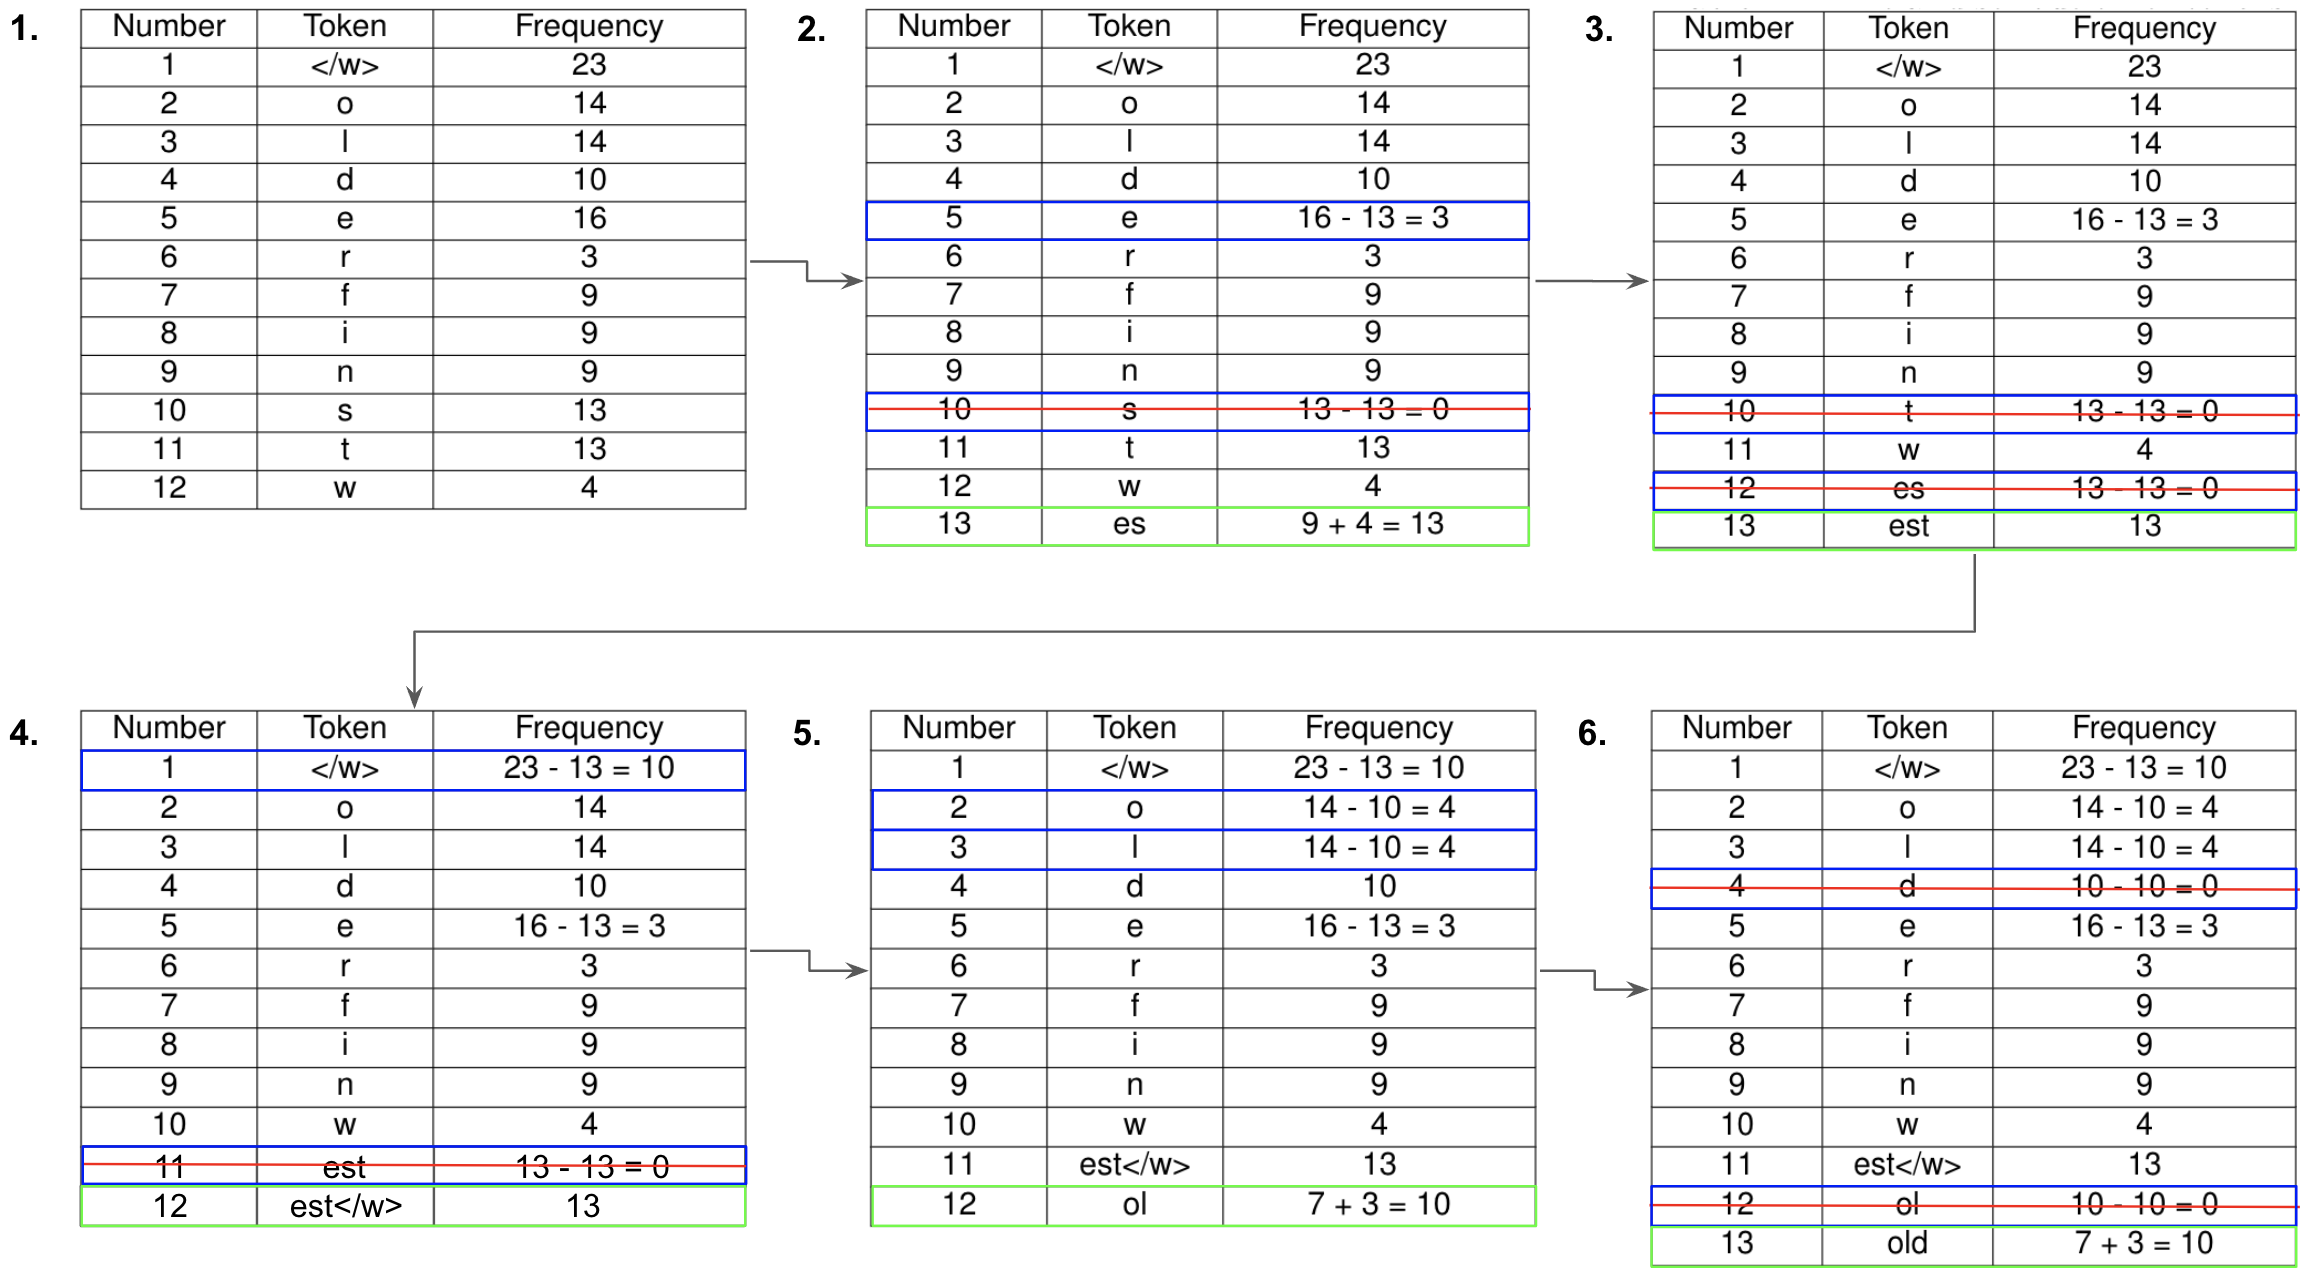
\includegraphics[keepaspectratio,scale=0.37]{chapter3_and_4_images/bpe_explained.png}
\caption{Steps of the BPE algorithm applied to an example corpus.}
\label{bpe_steps}
\end{figure*}

\begin{enumerate}
    \item The first step of the algorithm simply counts the number of characters in the corpus, assuming that each character defines a candidate token, i.e., as a character-level algorithm would behave. After that, the token pair frequencies are inferred, and the most frequent token pair is identified and added to the list of token candidates, as indicated at the bottom of table in the algorithm step 2.
    \item The most common token pair identified in the previous stage is $"es"$, occurring $9 + 4 = 13$ times. Thus, the tables entries related to the occurrence of these characters in a stand-alone fashion must be updated, simply by subtracting the number of common occurrences. Naturally, this happens to distinguish the occurrences of the single character tokens $e$ and $s$ and when $es$ happens, which are now separated. In this case, the row associated with $s$ is eliminated (represented by the red line), as it only spawns within the $es$ token
    \item In the step 3, a new token pair that spawns with the same frequency than $es$ is $est$, which by coincidence also contemplates all the occurrences of $es$ and $t$, leading to their elimination at this step
    \item In the next step, the merge of $est$ with $</w>$ results in the most frequent new candidate token having ($13$) occurrences. This merge results in a reduction of the frequency associated with $</w>$ to 10. 
    \item Another common token pair is $ol$, which has a frequency of $10$ in the given vocabulary. To represent this new token, the single characters $o$ and $l$ are subtracted by its number of occurrences, reducing their frequency to 4.
    \item In this step the token $old$ is formed, incorporating all the occurrences of $ol$ and removing the token $d$. Then, the process is interrupted due to the impossibility of fusing the candidate tokens. 
    \item Table \ref{final_distribution} summarizes the final tokens integrating the vocabulary. Note that the final vocabulary size ($11$) is inferior to the one considered at the start of this process ($12$).
\end{enumerate}

The main difference between this method and the ones derived from bi-gram segmentation is that it is capable of breaking words into interpretable units. Finding a clever way to split the words was one of the main challenges at that time. On the other hand, BPE is a greedy algorithm inspired in a compression algorithm with the same name, its purpose is biased towards reducing the size of the parameter vector, leading to some occurences wherein the subword tokens do not represent a morpheme with an enclosed meaning. However, despite having some meaningless tokens, the percentage of the ones that are meaningful are enough for it to stand out among the other techniques.

\begin{table}[h]
\caption{Final distribution of tokens (step 7)}
\fontsize{10}{12}\fontfamily{phv}\selectfont
\label{final_distribution}
\centering
  {\footnotesize
  \begin{tabular}{| P{0.1\linewidth} | P{0.1\linewidth} | P{0.2\linewidth} |}
    \hline
    Number & Token & Frequency \\
    \hline
    1 & </w> & 10 \\
    \hline
    2 & o & 4 \\
    \hline
    3 & l & 4 \\
    \hline
    4 & e & 3 \\
    \hline
    5 & r & 3 \\
    \hline
    6 & f & 9 \\
    \hline
    7 & i & 9 \\
    \hline
    8 & n & 9 \\
    \hline
    9 & w & 4 \\
    \hline
    10 & est</w> & 13 \\
    \hline
    11 & old & 10 \\
    \hline
\end{tabular}}
\end{table}
% https://amitness.com/2020/06/fasttext-embeddings/

The effectiveness of this approach is evaluated in \citet{sennrich-zhang-2019-revisiting}, which concentrates on evaluating the practical effects of changing word-level NMT to subword NMT using BPE. An ultra-low resource setting experiment was the one that benefited the most, raising a BLEU of 7.2 to 16.6 using the model of \citet{bahdanau2016neural}. 

\label{subword_variations}
\subsection{Subword variations}

Some research was also dedicated to using character-level RNNs only when the process of word-level embeddings generate a OOV word, as in \citet{DBLP:journals/corr/LuongM16}. Switching to character-level has also its drawbacks since character level spliting result in longer sequences of tokens wherein each one contains less information, yielding computational and modelling challenges. The most basic relates to the total memory required to represent a set of words in a character-level word representation, as it substantially increases as compared to subword or word-level solutions.

Sticking to an unique level of embedding is a paradigm broken in the work of \citet{chen-etal-2018-combining}, wherein different levels of granularity (word, subword and character) are combined to augment the token representations. These authors extended the encoder with a character-attention mechanism aiming to better learn source-side representations and incorporate information of of them into the decoder with a multi-scale attention, allowing the character-level information to cooperate with word-level to optimize the translation. Results show that such models when compared to the single granularity alternatives achieve higher scores, and the use of multiple levels also benefits it to address the OOV issue in one of their experiments.

Pre-trained word embeddings have also followed the trend with the work published by \citet{DBLP:journals/corr/BojanowskiGJM16}, which became popular under the name of \mbox{Fast Text}. This algorithm is inspired on \mbox{Word2Vec} based on the skipgram variant. It treats words as a bag of character n-grams and adds the special symbols ">" and "<" at the beginning and end of the words, respectively, to allow the algorithm to distinguish prefixes and suffixes from other character sequences. A visual distribution of the n-grams derived from the word "eating" is available at Table \ref{fast_text_ngrams}, where $n=6$.

\begin{figure*}[tb]
\centering 
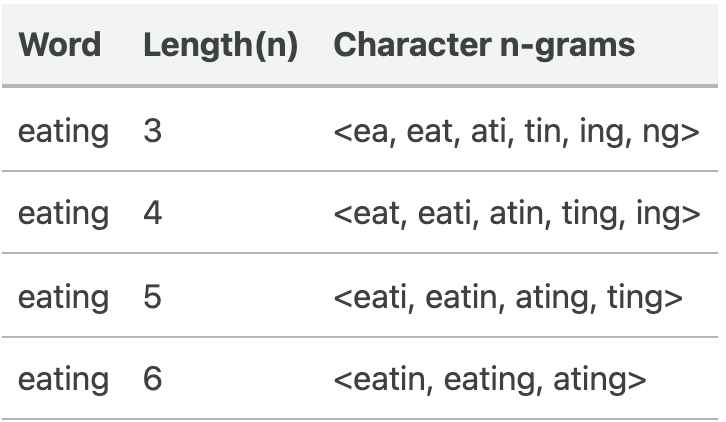
\includegraphics[keepaspectratio,scale=0.6]{chapter3_and_4_images/fast_text_ngrams.png}
\caption{N-grams generated by \mbox{Fast Text} for the word "eating"}
\label{fast_text_ngrams}
\end{figure*}

Basically, to each word is assigned a number of n-grams, and in practice only n-grams for $3 \leq n \leq 6$ are produced to each word. When the word representation is generated, it is represented by an index and a respective set of n-grams, which are called subword tokens. Finally, the word is represented by a sum of the vector representations correspondent to this set of n-grams.

\section{Transfer Learning}

Transfer Learning is a common practice in Machine Learning area, roughly consisting of reusing a model developed for a specific task as a starting point of a model dedicated to another task, typically reducing the complexity and time of the training process. This technique was exploited in \citet{zoph-etal-2016-transfer}, where weights associated to NMT models developed with a high-resource language pair are transferred to models targeting a low-resource language pair, both having English as the target language. By following this approach, the NMT model turns able to outperform the previous state-of-the-art Syntax-Based Machine Translation (SBMT) model. The metric used for evaluation was BLEU, and this happened in one of the four low-resource language tasks: the one involving the Hausa language.

Another transfer learning approach that may optimize the process of learning vector word representations is the use of pre-trained word embeddings. This may be achieved by adopting unsupervised language models to adjust their previously learned vectors and improve them within a $N$-dimensional space, where $N$ denotes the word-embedding size. The learned representations (weights) are then reused by the NMT model as starting values of its embedding layer, instead of proceeding with the random parameters' initialization typical in models trained from scratch.

The \mbox{Fast Text} algorithm presented in Section \ref{subword_variations} was the transfer learning strategy chosen for evaluation in this work, due to disposing of the benefits from the subword embeddings, analogous to the BPE. The use of such vectors for a warm start of a NMT model inherently enables it to be more robust against the OOV issue. The representations loaded in this case also have the advantage of carrying semantical and syntactical relations stored in the pre-trained language model.

An interesting work that analyses the effect of pre-trained word embeddings in low-resource scenarios is \citet{qi-etal-2018-pre}. The analysis conducted makes use of the same dataset considered in this work, TED Talks, which will be further described later. However, the model experimentally evaluated is based on \citet{bahdanau2016neural} and trained in a different framework as well as initialized differently than our work. 

One of the experiments analysed the effect of loading pre-trained word embeddings on reduced datasets, considering three distinct languages. The authors report that there is a "sweet spot" relative to the quantity of data available used for training that result in more efficient models. When loaded to a model trained with only 10\% of the TED Talks dataset, the pre-trained word embeddings have yielded small gains as compared to a random initialization. However, when trained over 30\% of the dataset, the BLEU gains suffer a peak, which monotonically decreases with the increase on this proportion of dataset instances used for training. 

Another experiment reported aims to enforce consistent embedding spaces across both languages, a technique called word embedding alignment. The authors exploit an approach that learns orthogonal transformations that convert the word embeddings of multiple languages to a common space, and use these transformed embeddings instead of the traditional learning process. These generated embeddings will be used as a starting point for the NMT model as usual. They achieve this by using linear geometrical transformations that normalize the vectors to the same range. Unfortunately, mixed results are reported, turning it hard to derive conclusions regarding its effectiveness. Some experiments report that pre-trained word embeddings are more effective when applied to more related language pairs (e.g. Portuguese-Spanish). 

Aiming to allow transfering the knowledge from language models trained on monolingual data to NMT, \citet{gulcere-language-model-nmt} proposes 2 solutions to fulfill this task: shallow fusion and deep fusion. The first uses a language model during decoding to rescore the candidate words that the translation model is considering as the next word to be predicted. The other one combines the decoder and language model which are coordinated with a controller mechanism. Unfortunately, the improvements reported are limited to the range of 0.5 up to 2 BLEU points in all experiments.

The results reported in the work \cite{qi-etal-2018-pre} for several language pairs in a range of scenarios seem to be more consistent, while the technique presented at \cite{zoph-etal-2016-transfer} is highly language and dataset dependent, as well as subjected to a high deviation. Therefore, there is some evidence that employing pre-trained word embeddings tend to be more effective than using transfer learning with a model trained on a different dataset.

\section{Data Augmentation}

The amount of parallel sentences is a key factor to the success of NMT, and data-hungry complex models may impose difficulties to the researchers aiming to contribute to this field. Unfortunately, large-scale parallel corpora is not available for the majority of the existing language pairs. On the other hand, it is much easier to obtain monolingual corpora. The Internet is a good example as disposing of a range of websites in multiple languages. This scenario motivated us to study data augmentation strategies to support the NMT task.

\subsection{Back Translation}

A branch of research in Data Augmentation is dedicated to the study of variations of the technique referred to as Back-Translation (BT)\abbrev{BT}{Back Translation}. In \citet{DBLP:journals/corr/SennrichHB15a}, the authors extract monolingual data corresponding to the target-side language, train a model to translate back to the source language and use it to build synthetical translations. Figure \ref{back_translation_figure} represents the augmentation process with a simplified representation. A NMT model is used to translate in the reverse direction (target to source language), generating artificial sentence pairs that are appended to the original dataset when training the main NMT model. 

\begin{figure*}[tb]
\centering 
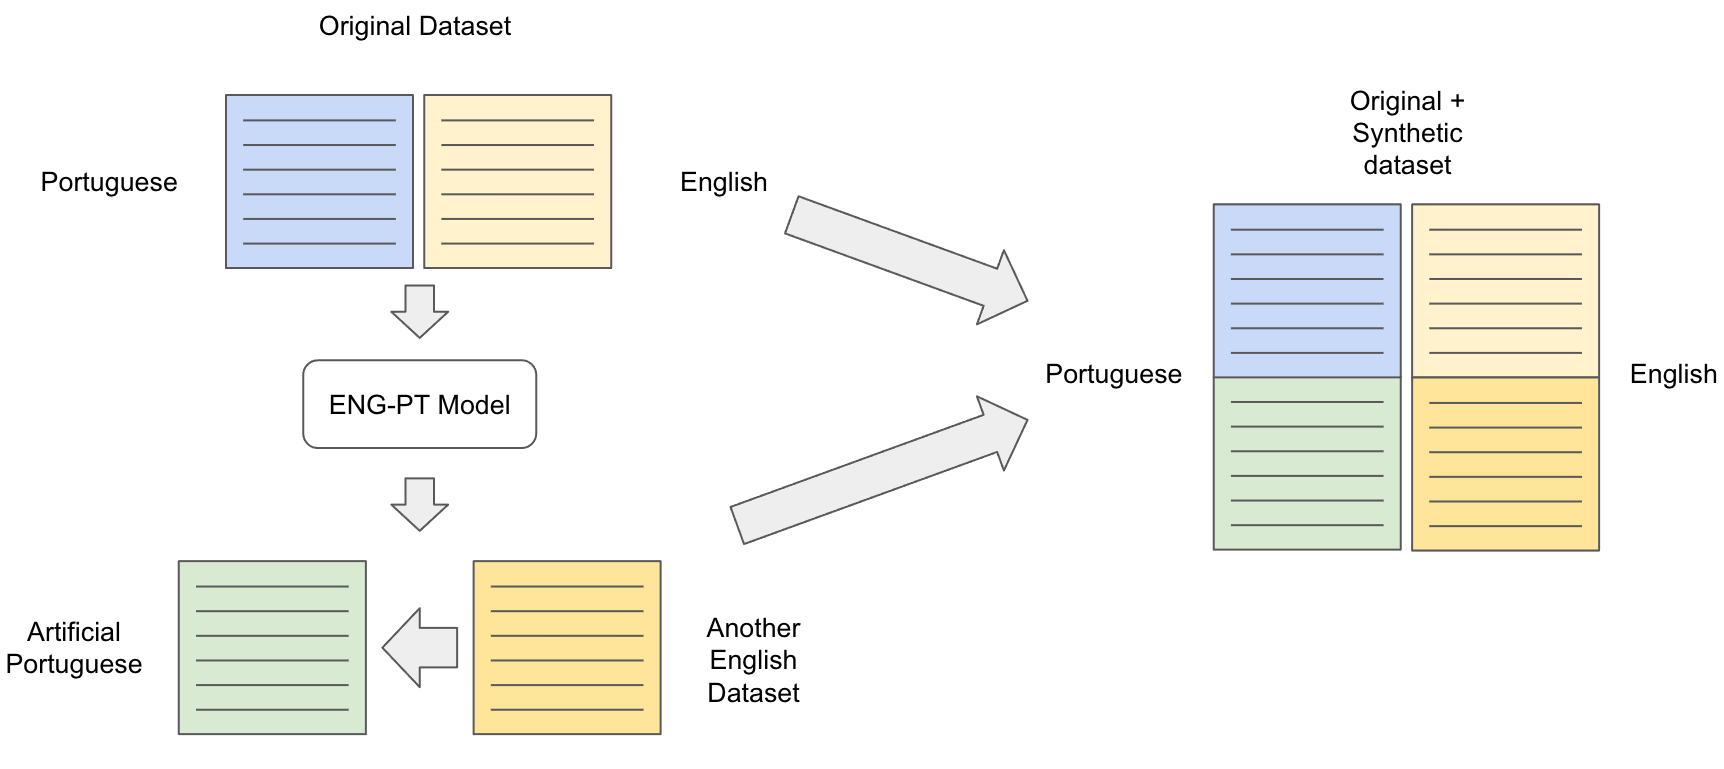
\includegraphics[keepaspectratio,scale=0.24]{chapter3_and_4_images/back_translation.png}
\caption{The Augmentation of a dataset with Back Translation}
\label{back_translation_figure}
\end{figure*}

BT has shown to be a simple, yet effective method to address low data availability in many domains, as shown in \citet{DBLP:journals/corr/abs-1804-06189}. This study concludes that the translation performance (measured with BLEU) is increased when a certain amount of synthetic translations are added, but this gain seems to tail off when the dataset balance is tipped too far in favour of the synthetic data.

In theory, the reason why the performance increases with the addition of artificial sentence pairs generated by another model is that when generating new synthetic pairs, "noise features" are added, which may be beneficial to learning. This sort of feature engineering technique in NMT is only beneficial in some cases. This strategy is only effective when the share of synthetic sentences is limited to a small portion of the whole dataset, thus keeping the "natural" sentences as the majority of instances. It is hard to define a rule to determine this ideal share, since it varies accordingly to the languages and text characteristics. Adding too much noise may compromise the models' performance, so this technique must be used with caution.

Different strategies for generating synthetic data are presented and compared in  \citet{DBLP:journals/corr/abs-1906-03785}. This study evaluates several augmentation methods in scenarios wherein English (ENG) is paired with high resource languages (HRL) and low resource languages (LRL). The strategies include techniques such as pivoting, word substitution (with the use of a dictionary) and an unsupervised NMT approach. A two-step pivoting method is also introduced: it uses a ENG-HRL model to create artificial HRL examples, and then use a HRL-LRL to create artificial sentences to the LRL. The authors propose methods to perform HRL-LRL translations which benefit from language characteristics such as word order. They claim that this ends up approximating better the true LRL sentences than using a ENG-LRL model. This technique has shown to be particularly useful for languages with even more restricted resources available than Portuguese. 

In some scenarios, this work reported that methods such as two-step pivoting may outperform back-translation. However, this study is limited to a few datasets and the gains reported in BLEU seem to not be expressive. Considering that consistent results are reported when other works apply the traditional back-translation in a wider range of datasets, we decided by this technique in favor of the two-step pivoting for addressing the low-resource issue in this work.

\chapter{Experiments on Neural Machine Translation}

The experimental investigation conducted in this work aim not only to report a possible score increase when applying technique a $X$ or $Y$, but also to address qualitative issues about the translations generated. The correlation between errors patterns and a specific technique is a process often overlooked in the NLP field, typically focused in optimizing one or more performance scores. Questions such as the following are not commonly addressed:

\begin{enumerate}
    \item How switching to a subword embedding may influence on the patterns of errors that a model makes?
    \item Is the sentence complexity or the incorporation of external knowledge a determining factor for model's performance? Do they induce some qualitative bias?
    \item Is it beneficial to augment the dataset with synthetic data (back translation)? How may the noise introduced by this procedure influence on the patterns of error produced by a model?
\end{enumerate}

These questions require a deeper analysis that goes over just matching words between the reference and the translations generated by the model, raising a demand for the definition of a categorization scale of the model's error with a linguistic focus. A contribution of this work is proposing a bidimensional criterion to assess the translation quality. The hypothesis raised here is that by analysing such patterns, we may enrich the insights that could be extracted from an experiment. 

Another goal of the same analysis is trying to understand the effects on the translation quality of the complexity level of the sentence, as from the dataset nature. In this direction, in our experiments, datasets from different domains were exploited to validate the hypothesis regarding the effectiveness of using datasets from distinct domains on BT. Another relevant factor that influenced on the choice of the datasets considered by this work are the limited GPU memory and data availability. In the following sections these experiments and their corresponding outcomes are described in greater details.

\section{Methodology}
\label{methodology}

Datasets with low to medium complexity levels were carefully selected for the proposed analysis: Tatoeba \cite{DBLP:journals/corr/abs-2010-06354} and TED Talks \cite{cettolo-ted-talks}. Both represent a low-resource scenario due to the scarce number of sentences, in alignment with some references \cite{sennrich-zhang-2019-revisiting} \cite{zoph-etal-2016-transfer}. Tatoeba is mainly constituted of basic to intermediate level English sentences, which can be interpreted as a corpus from a "school domain", ranging from elementary to middle school education constructions. The Tatoeba dataset contains $143.8$k small sentences with basic to intermediate English level, posing a low complexity challenge for the NMT task. It includes $26.3$k unique words in PT and $15.3$k in EN.

TED Talks is a medium-size dataset covering a range of subjects, including from low to highly complex sentences. It represents a mixed domain dataset, since it contains talks from experts on distinct areas. News Commentary v16 \cite{TIEDEMANN12.463} is a news focused domain monolingual dataset, used for BT in this work, and includes a rich range of sentences in terms of content and complexity.

%  \textcolor{red}{2. deveria colocar a métrica de palavras totais e palavras unicas pro dataset de ted talks?}

In the experiments, $10\%$ of Tatoeba was held out for testing, while the remaining data was split into 10\% for validation and $90\%$ for training, using a seed equal 0. Despite TED disposing predefined training, test, and validation sets, the original validation set is too small (906 sentences), leading us to move the last $20$ talks ($2081$ sentences) from the training set to this set. As a result, the training set contains $236.1$k ($1918$ talks) sentences, randomly sampled to define training batches using a seed equal to $157$, and the test set includes 11.4k sentences. Additionally, all text was pre-processed to eliminate all XML enclosed sentences and tags, except for the ones related to title and description.

The experiments were conducted using Python. Gensim was the library used to deal with word embeddings, and Spacy's Portuguese and English tokenizers were applied to the previously mentioned datasets. All experiments were performed on a single GPU, using the Google Colaboratory and Kaggle infrastructure. Typically such environments dispose of NVIDIA GPUs like Tesla P100, Tesla K80 or Tesla T4, with a GPU memory size ranging from 12GB to 16GB. 

Transformers is the architecture adopted in all experiments, and the parameters tuned for them are $d_{{model}}=256$, $d_{{ff}}=256$, 8 attention heads, and the $\mathbf{Q}$, $\mathbf{K}$ and $\mathbf{V}$ are square matrices with dimension $64$. The pre-trained \mbox{Fast Text}-based models, which employed the embeddings described in \cite{DBLP:journals/corr/abs-1708-06025} for Portuguese and \cite{fares-etal-2017-word} for English, are the only exceptions. In this case, both embeddings had  $d_{{model}}=300$ and 6 attention heads. The weights downloaded from the site published in the work of \citet{fares-etal-2017-word} were pre-trained on the Gigaword \cite{gigaword} corpus, considering the ID 16 option on the download list available at their website, after clicking on the repository tab. We chose this option as it was produced without lemmatization, as this technique is not applied when processing our datasets. All variants adopted the Adam optimizer with $\beta \in (0.9, 0.98)$ and $\epsilon = 10^{-8}$, a learning rate of $10^{-4}$ and the beam search considered a beam with size equal to 3. The early stopping criterion was based on the validation perplexity behaviour for ten epochs, halting the training in case of performance stagnation. During training, a new model was saved each time the best validation perplexity was achieved.

Regarding the BPE implementation, a toolkit developed by Google was preferred due to an interesting feature added over the original algorithm: it allows a priori vocabulary size definition instead of using the traditional number of merges. Sentencepiece \cite{DBLP:journals/corr/abs-1808-06226} is a language agnostic fast and lightweight implementation made in C++, widely used for subword segmentation. It was settled considering a maximum vocabulary size of $32$k tokens.

To assess quantitative performance, Sacrebleu \cite{post-2018-call} and NLTK \cite{Loper02nltk:the} were the BLEU variants exploited in our experiments. The major difference between them resides in a stronger Sacrebleu's penalization over cases to which the translated and reference sentences differ in length.

\section{Quantitative study}

To understand and evaluate the translation outcomes derived from a NMT model, both quantitative and qualitative aspects must be taken into account. To evaluate the former, scores such as Sacrebleu and NLTK BLEU provide distinct optics that allow to isolate the sentence length penalization variable. For the latter, the knowledge of an expert may help to break the problem into smaller parts, categorizing quality issues with the goal of capturing error patterns. 

The main goal of the experiments described in this section is to evaluate how the candidate techniques react to low-resource conditions quantitatively. The central idea resides in inferring which of them may help in circumventing issues that might arise in such cases and how to tune the auxiliary techniques based on a set of hyperparameters and setup conditions. To aid the reader on the task of following the rationale, it follows a brief summary describing all the experiments performed when conducting this evaluation process:

\begin{enumerate}
    \item The impact of restricted dataset content
    \begin{itemize}
        \item The experiment described in \ref{restricted_content_section} evaluates quantitatively the effect of several adverse limited data conditions on the NMT task performance
    \end{itemize}
    \item Effects of switching to subword level and ways of incorporating external knowledge
    \begin{itemize}
        \item In \ref{subword_external_knowledge}, a discussion regarding ways of loading pre-trained word embeddings and the effectiveness of switching to subword level (BPE) standalone is made. The experiments consider \mbox{Fast Text} and BPE strategies added to the Transformer
    \end{itemize}
    \item Effectiveness of Back Translation when addressing different low-resource settings
    \begin{itemize}
        \item The experiment shown in \ref{bt_conditions} evaluates the performance impact of using BT to extend a dataset, considering different synthetic shares for the dataset and exploiting data from the same or from a different domain
    \end{itemize}
    \item Comparison of Transformer candidates against the Google Translate benchmark
    \begin{itemize}
        \item The last experiment \ref{google_translate} compares the BLEU score of the aforementioned low-resource Transformer candidates with the output of the Google Translate service taken at the date of 11/01/2022
    \end{itemize}
\end{enumerate}

\subsection{The impact of restricted dataset content}
\label{restricted_content_section}

The process of training a model with constrained data may affect its performance in different ways. Therefore, different low-resource scenarios were created to try to unveal such effects. To shed light on such limitations, we considered a hypothetical experimental scenario, where only a fraction of TED and Tatoeba training sets are used in training. The following percentages were considered: 33.3\%, 50\%, 66.6\%, 83.3\%. 

This experiment has the aim of inferring if there is a minimum amount of sentences that a parallel dataset must have for the to model reach a good performance. It should become clear that after a certain size (or fraction, in this case) the additional performance obtained with the increase on the number of training instances is minimal, so alternatives must be explored to maximize model's performance. Table \ref{restricted_content} summarizes the outcomes of this experiment.

\begin{table}[h]
\caption{Performance obtained with models developed under restricted data (see text)}
\label{restricted_content}
\fontsize{10}{12}\fontfamily{phv}\selectfont
\begin{tabular}{| p{0.12\linewidth} | P{0.1\linewidth}  | P{0.07\linewidth}  | P{0.07\linewidth}  | P{0.07\linewidth}  | P{0.1\linewidth}  | P{0.07\linewidth}  | P{0.07\linewidth}  | P{0.07\linewidth} |}
    \hline
    \multirow{2}{2.0cm}{Fraction of the Dataset} & \multicolumn{4}{|c|}{Tatoeba} & \multicolumn{4}{|c|}{TED}\\
    \cline{2-9}
    & Sacrebleu & NLTK BLEU & Batch Size & Epochs & Sacrebleu & NLTK BLEU & Batch Size & Epochs \\
    \hline
    33.3\% & 48.64 & 67.09 & 512 & 76 & 24.7 & 57.65 & 30 & 40\\
    \hline
    50\% & 52.53 & 70.12 & 512 & 65 & 25.18 & 56.46 & 30 & 40\\
    \hline
    66.6\% & 55.3 & 72.12 & 512 & 58 & 26.22 & \textbf{56.81} & 29 & 36\\
    \hline
    83.3\% & 56.24 & 73.18 & 512 & 58 & \textbf{26.74} & 56.57 & 28 & 30\\
    \hline
    100\% & \textbf{57.99} & \textbf{74.07} & 512 & 58 & 25.24 & 55.36 & 28 & 30\\
    \hline
\end{tabular}
\end{table}

The results show that the Sacrebleu scores for the Tatoeba dataset were about twice the same as those achieved with TED, corroborating with the much higher complexity of the latter. The BLEU metrics for both datasets have shown a monotonic behaviour, with exceptions to TED in two cases: Sacrebleu (100\%  $\times$ 83.3\%) and NLTK (100\% $\times$ 83.3 and 83.3\% $\times$ 66.6 \%). The reasons for such findings may include: (1) the possible use of synonyms in the translations, an aspect ignored by any BLEU metric; (2) a higher incidence of Repetition errors due to data quality issues (to be discussed further in Section \ref{subjective_evaluation}); (3) the more complex and richer TED content, which might have led to a wider subject coverage in the training set, reducing model accuracy, a hypothesis requiring a future investigation. 

Models developed with a fraction of the original training datasets ($66.6\%$) performed surprisingly well, with the highest performance occurring at $100\%$ and $83.3\%$ for Tatoeba and TED, respectively. Besides, the competitive results in these cases as compared to $66.6\%$ indicates that the latter percentual may be sufficient for the model not suffering from low-resource data availability issues, but a more accurate percentage in each case requires a further investigation.

\subsection{Effects of switching to subword level and ways of incorporating external knowledge}
\label{subword_external_knowledge}

Aiming to evaluate the leveraging effects of pre-trained \mbox{Fast Text} and BPE \cite{DBLP:journals/corr/SennrichHB15} strategies in low-resource NMT tasks, BPE models were implemented exploiting the Texar framework  \cite{hu2019texar} (PyTorch version). In contrast, the alternative models considered customized PyTorch \cite{NEURIPS2019_9015} solutions. 

In practical terms, there are a range of alternatives when applying pre-trained word embeddings for NMT, thus identifying the most cost-effective approach can only be achieved experimentally. The main processing mechanism of the Transform model includes a embedding layer at the encoder and decoder blocks. The translation task is typically applied to a pair of distinct languages, hence one embedding will be used as the source language weights associated to this layer in the encoder, while the embedding from another language will perform similarly in case of the decoder. Another option is to replace the randomly initialized weights in either the encoder or the decoder, inducing the model to be trained from a "partial warm-start". 

Apart from the embedding strategy adopted, when loading the weights using the Gensim library, some optional parameters need to be specified in the $load\_word2vec\_format$ function: $binary$ and $unicode\_errors$. These parameters are set to $False$ and $"strict"$ by default, but the reference \cite{fares-etal-2017-word} recommends to load the embeddings using $False$ and $"replace"$. Both combinations were experimented to evaluate a possible impact over the performance scores, restricting only to the TED Talks dataset. Table \ref{transfer_learning_subword} exhibits the corresponding results, including in its first line the last one from Table \ref{restricted_content} to ease the comparison. All the \mbox{Fast Text} experiments used the default parameters, except for the $4$th entry of the table that used Fares' recommendations \cite{fares-etal-2017-word}.

\begin{table}[h]
\caption{Transfer learning and subword embeddings translation results}
\label{transfer_learning_subword}
\fontsize{10}{12}\fontfamily{phv}\selectfont
\begin{tabular}{| p{0.18\linewidth} | P{0.09\linewidth}  | P{0.06\linewidth}  | P{0.06\linewidth}  | P{0.07\linewidth}  | P{0.09\linewidth}  | P{0.06\linewidth}  | P{0.06\linewidth}  | P{0.07\linewidth} |}
    \hline
    \multirow{2}{2.2cm}{Technique applied} & \multicolumn{4}{|c|}{Tatoeba} & \multicolumn{4}{|c|}{TED}\\
    \cline{2-9}
    & Sacrebleu & NLTK BLEU & Batch Size & Epochs & Sacrebleu & NLTK BLEU & Batch Size & Epochs \\
    \hline
    None & 57.99 & 74.07 & 512 & 58 & 25.24 & 55.36 & 28 & 30\\
    \hline
    \mbox{Fast Text} (encoder of \cite{DBLP:journals/corr/abs-1708-06025}, randomly initialized decoder) with default package parameters & 56.96 & 69.91 & 512 & 50 & 24.07 & 61.69 & 30 & 45\\
    \hline
    \mbox{Fast Text} (encoder of \cite{DBLP:journals/corr/abs-1708-06025} + Gigaword decoder) with default package parameters & N/A & N/A & N/A & N/A & 24.54 & 61.76 & 32 & 89\\
    \hline
    \mbox{Fast Text} (encoder of \cite{DBLP:journals/corr/abs-1708-06025} + Gigaword decoder) with Fares' parameters \cite{fares-etal-2017-word} & N/A & N/A & N/A & N/A & 21.26 & 52.31 & 32 & 80\\
    \hline
    Subword BPE & \textbf{66.63} & \textbf{83.02} & 512 & 40 & \textbf{40.26} & \textbf{72.20} & 32 & 40\\
    \hline
\end{tabular}
\end{table}

Curiously, the adoption of \mbox{Fast Text} embeddings is related with an unexpected performance drop for both datasets. Conversely, the gains observed with BPE, which also exploits subword embeddings, were impressive. The variants following the recommendations \cite{fares-etal-2017-word} achieved worse performance than those related to default parameters.

One possible hypothesis for \mbox{Fast Text}'s bad performance is a possible overspecialization to other corpora domains, since it was produced with Internet data corpus mined by a crawler \cite{DBLP:journals/corr/abs-1708-06025}. The higher relative BPE gain with TED (15.02) as compared to Tatoeba (8.64) signalizes the effectiveness of BPE in dealing with more complex NMT scenarios, especially those involving a more diverse vocabulary, avoiding the OOV occurrences. 

\subsection{Effectiveness of Back Translation when addressing different low-resource settings}
\label{bt_conditions}

One hypothesis still unanswered is whether the noise inserted by a model when generating synthetic pairs may be beneficial to the performance of another model or not, and in what extent. Addressing this problem requires a experimental approach, since different domains, synthetic text ratios, natural languages and model characteristics constitute unique scenarios. The experiments covered in this section aim to answer questions like: What may be considered as an ideal synthetic ratio when applying BT? How the domain of the augmentation dataset impacts on the performance scores?

The experiments reported here are restricted to the TED dataset, since the low complexity of Tatoeba poses an easy challenge which may obfuscate possible higher gains of model performance. Data augmentation was performed with synthetic sentences produced with the own TED (using its left out sentences) and with the News dataset. These experiments aim to verify if data augmentation can help to reach higher BLEU scores under different low data availability conditions. 

Some scenarios of comparable models were created to evaluate the use of different domains versus the original (non-synthetic) dataset in the BT process. The motivation lies in understanding if the addition of extra data brings a boost in models' performance or even if it may compromise BLEU score. Datasets with different ratios of synthetic sentences were chosen, considering samples that contain 50\%, 33.3\%, 16.6\% and 8.33\% in terms of representivity. The artificial samples were generated by a single Transformer that translates to the reverse language pair, i.e. EN-PT, reaching 27.73 and 63.8 points for the Sacrebleu and NLTK scores, respectively. 

In addition, one extra BT variant was produced assuming a higher number of sentences than the original dataset size (120\%). This variant included 20\% of synthetic TED sentences, which somewhat makes it comparable to the 83.3\% + 16.6\% of TED dataset version, since both have the same synthetic ratio (20\%). The idea here was checking if adding more synthetic data on the top of the original dataset might enhance the previously reported scores. One last detail of this experiment is that the subset of back-translated sequences appended to the training sets was randomly sampled using the following seeds: 157 (TED) and 0 (News). Table \ref{tab:table3-bt-results} exhibits the results.

\begin{table}[h]
  \caption{TED Talks back-translation results}
  \fontsize{10}{12}\selectfont
  \label{tab:table3-bt-results}
  \centering
  {\footnotesize
  \begin{tabular}{| p{6.1cm} | p{1.4cm} |  p{1.8cm} | p{1.5cm} | p{1.1cm} | p{1.4cm} |}
    \hline
    Technique applied & Batch size & Epochs Trained & Sacrebleu & NLTK BLEU & Synthetic Ratio \\
    \hline
    None (Original TED) & 30 & 27 & 25.24 & 53.26 & N/A\\
    \hline
    \hline
    Reduction of TED to 50\% & 40 & 30 & 25.18 & \textbf{56.46} & N/A\\
    \hline
    BT (50\% of News synthetic examples) & 34 & 33 & 21.80 & 51.34 & 50\%\\
    \hline
    BT (50\% of TED synthetic examples) & 34 & 28 & \textbf{25.95} & 56.42 & 50\%\\
    \hline
    \hline
    Reduction of TED to 66.6\% & 36 & 29 & 26.22 & 56.81 & N/A\\
    \hline
    BT (33.3\% of News synthetic examples) & 34 & 27 & 24.12 & 53.77 & 33.3\%\\
    \hline
    BT (33.3\% of TED synthetic examples) & 34 & 27 & \textbf{27.54} & \textbf{58.95} & 33.3\%\\
    \hline
    \hline
    Reduction of TED to 83.3\% & 28 & 30 & 26.74 & 56.57 & N/A\\    
    \hline
    BT (16.6\% of News synthetic examples) & 34 & 29 & 31.28 & 63.30 & 16.6\%\\
    \hline
    BT (16.6\% of TED synthetic examples) & 34 & 27 & \textbf{34.62} & \textbf{64.61} & 16.6\%\\
    \hline
    \hline
    Reduction of TED to 91.67\% & 34 & 24 & 26.74 & 56.57 & N/A\\
    \hline
    BT (8.33\% of News synthetic examples) & 36 & 23 & 29.66 & 60.4 & 8.33\%\\
    \hline
    BT (8.33\% of TED synthetic examples) & 34 & 24 & \textbf{32.27} & \textbf{65.13} & 8.33\%\\
    \hline
    \hline
    Augmented TED (100\% of TED + 20\% of News) & 28 & 24 & 29.31 & 60.80 & 16.6\%\\
    \hline
\end{tabular}}
\end{table}
% \begin{table}[h]
%   \caption{TED Talks back-translation results}
%   \fontsize{10}{12}\fontfamily{phv}\selectfont
%   \label{tab:table3-bt-results}
%   \centering
%   {\footnotesize
%   \begin{tabular}{| p{6.1cm} | P{1.6cm} |  P{2.4cm} | P{1.5cm} | P{1.1cm} |}
%     \hline
%     Technique applied & Batch size & Epochs Trained & Sacrebleu & NLTK BLEU \\
%     \hline
%     None (Original TED) & 30 & 27 & 25.24 & 55.36\\
%     \hline
%     Reduction of TED to 50\% & 40 & 30 & 25.18 & \textbf{56.46}\\
%     \hline
%     BT (50\% of News synthetic examples) & 34 & 33 & 21.80 & 51.34\\
%     \hline
%     BT (50\% of TED synthetic examples) & 34 & 28 & \textbf{25.95} & 56.42\\
%     \hline
%     Reduction of TED to 66.6\% & 36 & 29 & 26.22 & 56.81\\
%     \hline
%     BT (33.3\% of News synthetic examples) & 34 & 27 & 24.12 & 53.77\\
%     \hline
%     BT (33.3\% of TED synthetic examples) & 34 & 27 & \textbf{27.54} & \textbf{58.95}\\
%     \hline
%     Reduction of TED to 83.3\% & 28 & 30 & 26.74 & 56.57\\    
%     \hline
%     BT (16.6\% of News synthetic examples) & 34 & 29 & 31.28 & 63.30\\
%     \hline
%     BT (16.6\% of TED synthetic examples) & 34 & 27 & \textbf{34.62} & \textbf{64.61}\\
%     \hline
% \end{tabular}}
% \end{table}

One may readily infer that the increasing score trend switches its behaviour, depending on the size of the synthetic portion with respect to the whole dataset. For a more severe restriction on the dataset size (50\%), using other-domain synthesized sentences is harmful to model performance, while own-domain synthesis resulted in a marginally better BLEU score. However, for a lower percentage of synthetic data, positive effects start to appear. Considering a less significant restriction ($\approx 33 \%$), using the same domain sentences in back-translation led to a mild increase in both BLEU values when compared to the Original TED, signalizing that such "noisy" sentences may contribute to increasing the translation quality. When applying an intermediate restriction ($\approx 16.6 \%$), the approaches from both domains are quite effective, resulting in models that largely surpass the model developed over the original data. Finally, when considering a small restriction ($\approx 8.3 \%$), the monotonic behaviour of scores related to same data domain augmentation switches its trend and starts decreasing, but still representing an improvement over the benchmark. Regarding augmentation with synthesized data from other domain, the score also decreases similarly. It is important to emphasize that the scores of all variants were generated using the same test data, otherwise the comparison would not be fair.

One intriguing outcome of this experiment was that the Transformer variant trained on a larger dataset behaved unexpectedly by performed worse than variants considering the same synthetic ratio on smaller datasets. The decrease in BLEU was significant: more than 5 points (34.62 vs 29.31) when compared to the 83.3\% TED version. On the other hand, when considering the Transformer trained on the original dataset, the addition of 20\% of News data enhanced the original models' performance. One possible hypothesis to explain this, but that deserves further investigation, is that since the TED dataset includes mixed domain content, the last piece of the dataset (about 16\%) may contemplate texts with a vocabulary pretty decorrelated to the remaining dataset parts. The addition of more back translation data may also lead to an increase on the model's performance, but exploring this further will remain as a proposal for future work.

\subsection{Comparison of Transformer candidates against the Google Translate benchmark}
\label{google_translate}

To evaluate how efficient were the previous stategies in tackling low-resource issues, we compare these models with a benchmark that isolates this limitation. The comparison is crucial to understand how well the model has mitigated issues related to such restricted domains. Therefore, Google Translate was used as a reference benchmark. Table \ref{google-translate-comparison} shows the results for BLEU considering the best performing model candidates among the previous experiments, and for this benchmark.

\begin{table}[h]
  \caption{Performance comparison between our best performing models and Google Translate}
  \fontsize{10}{12}\fontfamily{phv}\selectfont
  \label{google-translate-comparison}
  \centering
  {\footnotesize
  \begin{tabular}{| p{6.1cm} | P{1.6cm} |  P{2.4cm} | P{1.5cm} | P{1.1cm} |}
    \hline
    Model & Batch size & Epochs Trained & Sacrebleu & NLTK BLEU \\
    \hline
    Transformer (Original TED) & 30 & 27 & 25.24 & 55.36\\
    \hline
    Subword BPE & 32 & 40 & \textbf{40.26} & \textbf{72.20}\\
    \hline
    Reduction of TED to 83.3\% & 28 & 30 & 26.74 & 56.57\\    
    \hline
    BT (16.6\% of News synthetic examples) & 34 & 29 & 31.28 & 63.30\\
    \hline
    BT (16.6\% of TED synthetic examples) & 34 & 27 & \textbf{34.62} & \textbf{64.61}\\
    \hline
    Google Translate (used on 11/01/2022) & Unknown & Unknown & \textbf{52.19} & \textbf{78.74}\\
    \hline
\end{tabular}}
\end{table}

Considering the Sacrebleu BLEU metric that includes sentence length penalization, our best model reached 77.1\% of Google's performance, making use of a model and computational infrastructure many orders of magnitude inferior in terms of computational power and costs, to the one associated with Google's model. When switching to the NLTK metric, which ignores the sentence length, the gap between them significantly reduces, as this ratio goes up to 91.69\%. We must stress that the current Google model is able to identify even disease acronyms, such as ACS (Acute Coronary Syndrome), one achievement almost impossible to be reached for models developed over only one low-resource dataset. This model is even able to predict translations having just part of the word as input.

Unfortunately, there is not much to be said regarding the underlying techniques that empower Google's model. The last papers over this topic that were made available suggest the use of a RNN-based encoder and a decoder with attention, but the type of attention mechanism is not mentioned. When looking at more recent information, based on a blog post of \citet{google-ai-2020}, they grant a relevant increase in BLEU to the use of back-translation techniques, specially for low-resource languages. The latest papers available are heavily outdated \cite{DBLP:journals/corr/JohnsonSLKWCTVW16} \cite{DBLP:journals/corr/WuSCLNMKCGMKSJL16} and the techniques have probably been deprecated or updated somehow. Recent updates are mostly reported in blogs, with the latest one summarizing their Artificial Intelligence achievements in 2021 \cite{google-ai-2022}, with some mentions to the new Google Translate features, such as the efforts towards reducing the gender bias.

The Google Translate model is probably built upon a carefully curated set of techniques and parameters. One possibility to bridge the gap between it and other models is to try a combination of the discussed low-resource strategies, although there are no guarantees that their positive benefits would necessarily be constructive when combined. As the main goal from this work is more focused on qualitative outcomes, and not in boosting performance score as far as possible, we focused our energy in quantifying and interpreting patterns of translation errors. The next section provides more detail of such attempts.

\section{Qualitative study}
\label{subjective_evaluation}

Understanding a problem through the lens of a quantitative methodology can already yield a range of findings, but engineers often underestimate the potential of a qualitative approach to complement such analysis. In modern tech companies, both methodologies are commonly used together to provide a richer view of the problem, which would be too restricted by solely considering a qualitative focus. When speaking of product management, for instance, designers and analysts are the left and right arms of a manager, for evaluating a scenario of interest in a qualitative and quantitative way, respectively. The same analogy can be applied here, where computational researchers working on the Natural Language domain often refer to linguistics experts to better address and solve a language related problem.

\subsection{Challenges of a qualitative analysis}

When performing Machine Translation, a number of language, model specific and data availability nuances might pose a range of challenges with a high potential of hindering qualitative analysis results. Most of them are fairly widespread and well-known by most researchers in this area, but depending on whether the dataset has been curated, how much of its biases have been identified and addresses, and also how well dimensioned it is; the struggle to create high quality translations can increase significantly. 

The first challenge are data quality issues, such as references that do not match the exact expected translations, and may even contain some errors. Data quality issues have a significant impact on the ability to correctly evaluate the translations from a model, and of course, they are also scattered throughout the TED Talks dataset \cite{cettolo-ted-talks}. Such data quality issues can also intensify some known flaws of using BLEU for evaluation, such as its lack of ability to catch synonyms an overestimated loss score due to human translation biases. Table \ref{reference_errors} shows some sentences arbitrary selected from the TED Talks database that illustrates these issues.

\begin{table}[!htp]
  \caption{Selected references with errors}
  \fontsize{10}{12}\fontfamily{phv}\selectfont
  \label{reference_errors}
  \centering
  {\footnotesize
  \begin{tabular}{| p{0.35\linewidth} | P{0.35\linewidth} |  P{0.2\linewidth} |}
    \hline
    Original Sentence (PT) & Reference & Suggested Correction \\
    \hline
     A medida que fazíamos nossas futuras expedições Eu estava vendo criaturas em fontes hidrotermais e às vezes coisas que eu nunca tinha visto antes, às vezes coisas que ninguém tinha visto antes, que realmente não haviam sido descritas pela ciência no momento em as vimos e as \textbf{imaginamos}. & As we did some of our subsequent expeditions, I was seeing creatures at hydrothermal vents and sometimes things that I had never seen before, sometimes things that no one had seen before, that actually were not described by science at the time that we saw them and \textbf{imaged} them. & Switch \textbf{imaged} to \textbf{imagined}. \\
    \hline
    Fico feliz em dizer que não temos este tipo de situação – um cirurgião com quem conversei alguns anos atrás que tinha trazido para aqui gêmeos xipófagos a fim de separá-los, em parte para ficar famoso. & I'm glad to say we don't have the kind of situation \textbf{with} - a surgeon I talked to a few years ago who had brought over a set of conjoined twins in order to separate them, partly to make a name for himself. & Remove \textbf{with} from the reference. \\
    \hline
    Fomos para \textbf{São Paulo} onde os outdoors foram banidos. & We went to \textbf{San Paulo} where they have banned outdoor advertising. & Correctly represent the São Paulo city with its original name, without the tilde: Sao Paulo. \\
    \hline
\end{tabular}}
\end{table}

All models show some sort of error patterns after being evaluated with a number of curated sentences, which are not usually trivial to explain. Besides, splitting a qualitative analysis into smaller and focused aspects that can be addressed and assessed by a bidimensional criterion also is not also straightforward. However, the better the answer found to this problem, the better the proposed analysis can provide insights about models' performance, especially in a practical sense. This scenario raises a second challenge, regarding how to set the breadth and depth of the qualitative criterion used. To address the complexity of defining such a criteria, the help of an expert on the field is mandatory. These issues motivated us to hire someone with 9 years of teaching and translating experience in English, that describes himself as a C1 level english speaker, according to the CEFR scale \cite{COE}.

The participation of a translator in this work was a rewarded interaction. In other words, he was called on demand to help, and the whole process was constrained by my personal budget available for it. Since all the interactions were conducted autonomously, without any type of sponsoring, the amount of evaluated sentences and thus the generalization power of the analysis is somewhat restricted despite highly valuable in terms of innovation in this field.

Part of the qualitative work conducted here was dedicated to understanding whether text complexity does influence the error patterns when generating translations or not. This led the translator to categorize Ted Talks database instances in different levels according to the CEFR scale \cite{COE}, which will better detailed in a specific section ahead. 

The process of creating a qualitative bidimensional criterion turned out to be the third challenge, especially regarding how to avoid a stronger inductive bias, i.e. biases not inherently related with the reference, but with the qualitative criterion itself. The consulted translator defined some categorization ideas, but understanding his rationale and giving feedbacks while avoiding to not bias the final decision has demonstrated to be a very subtle process. 

The bias question is also strongly linked to the process of sampling database instances: samples had to be curated to match the expected complexities and reach a certain number of excerpts per complexity. Random choices of excerpts were picked when performing this task to avoid bias, demanding a lot of manual work. However, when getting near the pre-established goal of 15 excerpts, the approach demanded a more flexible conduction. Whenever a pair of excerpts was near the threshold between two adjacent complexity levels, we had to discuss whether it could be switched to the level requiring more samples or if it should remain. 

It is worth to emphasize that 100 distinct pairs of sentences were considered in this analysis, but the total number of evaluations is quite higher, as the candidates have changed in the first steps taken. Also, a higher number of models than what is actually reported was selected for the qualitative experiments, because we had to evaluate their pattern of errors and decide upon keeping them or keep exploring. Increasing the number of evaluated sentences was also necessary to cover all the complexity levels. Ensuring that all the main types of errors are covered in our sample of the dataset was the ultimate goal. The clusters defined by each qualitative criterion should be well-scoped and avoid intersections to bypass a potential interpretability loss. The discussion for both complexities and qualitative criteria was fruitful as it helped to better grasp the consistency of the criteria chosen as the samples were evaluated.

% During the production of the thesis, all the quantitative and qualitative interactions performed with the thesis advisor and translators respectively happened in parallel. Everything kept going while the main author also worked in private companies, given that this thesis is the result of a part-time enrollment in the electrical engineering masters course. The whole production process suffered from time and availability constraints because of those peculiarities, something we call a human factor low-resource limitation.

\subsection{The qualitative criteria}

As previously mentioned, 2 qualitative dimensions were created to validate the hypothesis stated in the beginning of the chapter and provide more clarity: sentence complexity and error patterns. One relevant hypothesis raised before that is still to be addressed is that error patterns performed by the same model in different text domains (or subjects) and text complexities may change. We have chosen to complement the error patterns with the sentence complexity levels aiming to isolate the effects of both and be better prepared to validate our initial hypothesis. Another intent behind complexity segmentation is that it also should help to better understand associations between text complexity and the error patterns of the techniques exploited. Finally, defining and clustering potential errors generated by the models belong to the core of this work, so it was considered as a mandatory dimension.

\subsubsection{Setting the classes of errors}

To analyse the patterns of errors generated by the model, a multicategorical criterion was created along with a human translator to cluster the types of errors. Eight categories were considered: Reference Matching, Omission, Out of Context, Verb Tense, meaning deviation, Insertion, Repetition and $<$unk$>$ errors. A detailed error description of each category can be found at Table \ref{error_classes}.

\begin{table}[!htp]
\caption{Description of the classes of errors defined in the process of error analysis}
\fontsize{10}{12}\fontfamily{phv}\selectfont
\label{error_classes}
\centering
  {\footnotesize
  \begin{tabular}{| p{0.15\linewidth} | p{0.8\linewidth} |}
    \hline
    Error class & Description \\
    \hline
    Reference matching & A similar, but different word from the reference is used in a context to which the sentence can still be understood, or the order of words are switched. \\
    \hline
    Omission & Corresponds to ocassions wherein part of the source sentence is ignored by the model. Consequently, the translated sentence does not integrate the corresponding content. \\
    \hline
    Out of context & The model uses a word that doesn’t fit in the surrounding context, and the translation loses cohesion. This error also contemplates nonexistent words created by BPE. \\
    \hline
    Verb tense & When conjugating a verb, the model misses to capture the right tense and changes it on its guess, generating an innaccurate translation. \\
    \hline
    Meaning deviation & The model translates a sequence of words that is way different from the expected translation. This usually happens when several words are changed and the sentence is rephrased to preserve cohesion between these new words, resulting in a loss of meaning when compared to the source sentence. \\
    \hline
    Insertion & This category indicates that the algorithm has inserted words that are unnecessary given the context. \\
    \hline
    Repetition & Happens when the likelihood estimate of the next translation becomes biased, inducing the model to keep translating the same set of words more than once. \\
    \hline
    $<$unk$>$ & The traditional token that a model outputs whenever none of the words known by it would fit in a given context. \\
    \hline
\end{tabular}}
\end{table}

Recall that the $<$unk$>$ error classification is inside the list but it naturally happens when the model sees a word during inference that wasn't presented during training. This category was kept as it influences how the model tunes cohesion and coherence in a sentence. All the sentences evaluated were then classified under these 8 classes of errors. For the sake of illustration, Table \ref{error_examples} shows some cherry-picked sentences and their correspondent evaluation regarding error classes.

\begin{table}[h]
  \caption{Examples of wrong translations classified according to the proposed error criteria}
  \label{error_examples}
  \centering
  {\footnotesize
  \begin{tabular}{| p{3.0cm} | P{2.8cm} | P{2.5cm} | P{4.5cm} |}
    \hline
    Original sentence & Reference & Model outcome & English error diagnostic \\
    \hline
    E porque isso é verdade? & 
    And why is it true? & 
    And why is this true? &
    \textbf{Reference matching error}: Switched "it" for "this", without losing meaning. \\
    \hline
    Michael Specter: O perigo da negação da ciência. & 
    Michael Specter: The danger of science denial. & 
    Michael <unk>: the danger of science. & 
    1) Omission error: denial. 2) $<$unk$>$ error: Specter was interpreted as an unknown token. \\
    \hline
    Mas, na verdade, nós somos mudados. Somos marcados, sem dúvida, por um desafio, quer físicamente, emocionalmente, ou ambos. & 
    But, in fact, we are changed. We are marked, of course, by a challenge, whether physically, emotionally or both. & 
    But in fact, we're changed. We're <unk>, of course, by a challenge, whether we can physically, emotionally, or both. &
    1) \textbf{Omission error}: The model omitted "marked". 2) \textbf{Out of context error}: The model added "can", completely changing the original meaning of the sentence 3) \textbf{$<$unk$>$ error}: "marked" wasn't successfully translated. \\
    \hline
    Ganhamos um monte de prêmios. & 
    We've won a bunch of awards. & 
    We won a bunch of awards. We won a lot of awards. &
    1) \textbf{Verb tense error}: Switched Present Perfect "we've won" for Simple Past "we won". 2) \textbf{Repetition error}: "We won a lot of awards" was inserted, repeating the original reference's meaning. \\
    \hline
    E exigiu muita preparação, tivemos que construir câmeras e luzes e todo tipo de coisas. & 
    And it took a lot of preparation, we had to build cameras and lights and all kinds of things. & 
    And it was a lot of please, we had to build cameras and lights and all kinds of things. &
    \textbf{Meaning deviation error}: The model switched "it took a lot of preparation" for "it was a lot of please". \\
    \hline
    A mesma coisa, só que maior. & 
    Same thing, only bigger. & 
    The same thing, only bigger than that. &
    \textbf{Insertion error}: The model inserted "the" and "than that" in the translation. \\
    \hline
\end{tabular}}
\end{table}

The selected examples are low in complexity and focused on being didactic. They contain simpler mistakes than the average, as the goal is just to illustrate the error categories' descriptions. A small piece of text containing many errors makes the process of distinguishing between these error categories even harder, which would compromise the didactic purpose of Table \ref{error_examples} and might increase the chance of mislabelling. Another factor that contributes to the same issue is the sentence complexity, which is covered as one of the qualitative pillars of the analysis.

\subsubsection{Setting the complexity categories}

To define the dataset instances included in this qualitative analysis, random samples were selected from TED, analysed by the human translator, and stratified according to the CEFR scale \cite{COE}. Due to dataset characteristics, this study restricted its coverage to sentences classified as A1, A2, B1 and B2. A very few sentences were classified as from the C1 and C2 levels in this set: less than 5 samples from a total of 100 analysed sentences. As time and budget were natural limitations, we decided to remove them from the experiments. Thus, from the 100 distinct sentences evaluated, 60 were used for the experiments performed in this work, with 15 belonging to each category of complexity.

Categorizing sentences solely based on the general descriptions available for the CEFR levels is a hard task. Table \ref{evaluation_examples} illustrates cases found in this analysis, with the corresponding complexity assigned by the translator and the rationale behind this classification according to him. It helps in the task of absorbing the scope of the qualitative criteria, since it has one sample per complexity level and most of the errors are classified and the reason for that is exposed.

\begin{table}[h]
  \caption{Evaluation of some translated sentences}
  \label{evaluation_examples}
  \centering
  {\footnotesize
  \begin{tabular}{| p{2.2cm} | P{2.4cm} | P{2.0cm} | P{1.0cm} | P{1.8cm} | P{3.2cm} |}
    \hline
    Original sentence & Reference & Model guess & Model Type & Complexity and reason & English error classification \\
    \hline
    Você não muda nunca, né? & 
    You never change, do you? & 
    You don't change it, do you? & 
    Transformer with BPE & 
    A1 - Simple present & 
    1) Insertion: it was added. 2) Reference matching: Never/Don't are close in meaning \\
    \hline
    Tente perguntar coisas assim: "Como é que foi aquilo" ? & 
    Try asking them things like, "what was that like?" & 
    Try to ask things like this: "how is it that?" & 
    Transformer with BPE & 
    A2 - ING used as infinitive and intermediate level question in Simple Past & 
    1) Verb Tense: switched "try asking" (continuous) for "try to ask" (infinitive). 2) Omission: "them". 2) Insertion: "this". 3) Meaning deviation: "what was that like?" was changed to "how is it that?" \\
    \hline
    E vocês sabem, uma epifania é normalmente algo que encontramos que tínhamos deixado cair em algum lugar. & 
    And you know, an epiphany is usually something you find that you dropped someplace. & 
    And you know, an epiphany is normally something that we've found that we'd left somewhere. & Transformer 66\% of TED & 
    B1 - Simple present and simple past, with uncommon vocabulary & 
    1) Reference matching: usually/normally. 2) Meaning deviation and Verb tense: "we've found that we'd left somewhere" lost both its original meaning and tense \\
    \hline
    Ele tinha acabado de ouvir a primeira e a quarta sinfonia de Beethoven, e veio até o backstage se apresentar. & 
    He had just heard a performance of Beethoven's first and fourth symphonies, and came backstage and introduced himself. & 
    He'd just heard the first one and the fourth symphony of Beethoven, and came to the $<$unk$>$ to introduce him. & 
    Trans-former 33\% of TED & 
    B2 - Past perfect and past simple & 
    1) Omission: The model omitted "a performance of" that appears in the original sentence. 2) Unk error. 3) Insertion: "first \textbf{one}". \\
    \hline
\end{tabular}}
\end{table}

We must stress that there are no clear hard rules to describe the thought process behind choosing a given complexity category or error class. The existence of some error patterns tends to favour the evaluation towards a label, but a broader evaluation and richer exploratory analysis would be necessary to define more embracing and generic rules. Some other sentences are available in a separate repository for a more interested reader\footnote{Detailed error descriptions and some evaluation samples can be found at \url{https://github.com/Art31/pt-nmt-low-resource.git}.}.

\subsubsection{Design of experiments}

The classification in error classes and complexity levels for all the 60 sentences culminated in a dataset with a lot of binary columns labelling each sentence regarding the occurrence or not of each one of the qualitative categories. It isn't trivial to extract insights from these outcomes by simply inspecting the ordinary frequencies observed for this dataset in its raw form, as there are bidimensional associations that couldn't be easily identified or described by this way. This issue motivated us to use dimensionality reduction and clustering techniques to unveil bidimensional patterns. 

The set of experiments dedicated to clarify the translation error patterns was carefully thought to evidence possible associations between the model candidate, sentence complexity and their respective class of error patterns. To guide the reader over the qualitative analysis, below there is a summary of the experiments performed :

\begin{enumerate}
    \item Statistical hypothesis test over the proportion of errors commited by each model
    \begin{itemize}
        \item Multiple Fisher exact tests are used to infer whether come particular model and technique combination indeed contributes to mitigate some modalities of errors, or maybe if a given model is more prone to producing an error than others or not
    \end{itemize}
    \item Hierarchical clustering analysis
    \begin{itemize}
        \item Bimensional associations between the errors, models and sentence complexity are evaluated in this experiment aiming to shed light on possible error patterns from each technique
    \end{itemize}
    \item Correspondence analysis
    \begin{itemize}
        \item This algorithm also drives bidimensional conclusions on the qualitative side, with a visual 2-D representation that enables interesting visual interpretations, complementing the previous analysis
    \end{itemize}
\end{enumerate}

In the following experiments, only one of the Back Translation Transformers generated in this work is considered. The model there referred to as BT is the Transformer trained on a dataset composed 83.3\% of the original TED and 16.6\% of the other part of the same dataset subjected to BT.

\subsection{Error proportion analysis with Fisher Exact test}

The purpose behind this experiment is to understand if given the error occurrences we can assume that one variant is biased to a specific error class, with statistical significance. An appropriate hypothesis test was chosen for this goal, given the limited sample size: the Fisher Exact Test. Fifteen sentences from each complexity level were presented to all 4 candidate models: (1) the best Back Translation variant, trained on 83.3\% of TED augmented with 16.6\% of TED data, (2) the Transformer trained over a fraction of $33\%$ of TED, (3) the Transformer trained on $66.6\%$ of TED and (4) the BPE variant, trained over the entire dataset. 

The rationale for using such candidates is based on their performance on the previous experiments and the structural differences between them. We must recall that one of the hypothesis is whether switching to the subword level and using data augmentation leads to an impact in our qualitative indexes. This analysis also included the reduced TED Transformers to evaluate possible effects of restricting the dataset size over the error patterns.

Table \ref{error_classes_per_model_and_complexity} depicts the number of errors committed by each model, stratified by sentence complexity and error category. Considering the limitations of this analysis, such as the reduced sample size and the availability of only one translator, all models performed quite similarly regarding the Omission and Verb Tense occurrences. Nonetheless, BPE stands out by having the lowest average occurrence of Insertion, Repetition and Omission errors. Curiously, the Back Translation variant has the highest occurrence of Out of Context and Reference Matching errors, which may be an influence of using of artificial data. Both Transformers trained on reduced TED have a very similar distribution of errors considering the error types as their averages are usually very close, indicating that these low-resource constraints may have a diminished impact on their errors patterns.

\begin{table}[!htp]
\caption{Ratios of class errors per dataset and sentence complexity (see text)}
\fontsize{10}{12}\fontfamily{phv}\selectfont
\label{error_classes_per_model_and_complexity}
\centering
\begin{tabular}{| p{0.8cm} | P{1.29cm}  | P{1.45cm}  | P{1.0cm}  | P{1.0cm}  | P{1.0cm}  | P{1.35cm}  | P{1.0cm}  | P{1.0cm} |  P{1.0cm} |}
    \hline
    Model Name & Complexity & Reference Matching & Omission & Out of context & Verb tense & Meaning deviation & Insertion & Repetition & $<$unk$>$ error\\
    \hline
    \multirow{5}{1.2cm}{BT} & A1 & $\nicefrac{6}{15}$ & $\nicefrac{3}{15}$ & $\nicefrac{1}{15}$ & $\nicefrac{1}{15}$ & $\nicefrac{0}{15}$ & $\nicefrac{1}{15}$ & $\nicefrac{0}{15}$ & $\nicefrac{1}{15}$\\
    \cline{2-10}
    & A2 & $\nicefrac{13}{15}$ & $\nicefrac{7}{15}$ & $\nicefrac{2}{15}$ & $\nicefrac{4}{15}$ & $\nicefrac{3}{15}$ & $\nicefrac{6}{15}$ & $\textbf{\nicefrac{1}{15}}$ & $\nicefrac{3}{15}$\\
    \cline{2-10}
    & B1 & $\nicefrac{13}{15}$ & $\nicefrac{5}{15}$ & $\textbf{\nicefrac{3}{15}}$ & $\nicefrac{5}{15}$ & $\nicefrac{5}{15}$ & $\nicefrac{5}{15}$ & $\nicefrac{0}{15}$ & $\nicefrac{3}{15}$\\
    \cline{2-10}
    & B2 & $\textbf{\nicefrac{15}{15}}$ & $\textbf{\nicefrac{11}{15}}$ & $\nicefrac{0}{15}$ & $\textbf{\nicefrac{11}{15}}$ & $\textbf{\nicefrac{7}{15}}$ & $\textbf{\nicefrac{10}{15}}$ & $\textbf{\nicefrac{1}{15}}$ & $\textbf{\nicefrac{8}{15}}$\\
    \cline{2-10}
    & Average & 78.3\% & 43.3\% & 40.0\% & 35.0\% & \textbf{25.0\%} & 36.6\% & \textbf{3.3\%} & \textbf{25.0\%}\\
    \hline
    \multirow{5}{1.2cm}{33\% TED} & A1 & $\nicefrac{5}{15}$ & $\nicefrac{3}{15}$ & $\nicefrac{0}{15}$ & $\nicefrac{2}{15}$ & $\nicefrac{3}{15}$ & $\nicefrac{7}{15}$ & $\nicefrac{4}{15}$ & $\nicefrac{4}{15}$\\
    \cline{2-10}
    & A2 & $\nicefrac{11}{15}$ & $\nicefrac{7}{15}$ & $\textbf{\nicefrac{5}{15}}$ & $\nicefrac{4}{15}$ & $\nicefrac{4}{15}$ & $\nicefrac{6}{15}$ & $\nicefrac{2}{15}$ & $\nicefrac{5}{15}$\\
    \cline{2-10}
    & B1 & $\nicefrac{13}{15}$ & $\nicefrac{9}{15}$ & $\textbf{\nicefrac{5}{15}}$ & $\nicefrac{6}{15}$ & $\nicefrac{8}{15}$ & $\nicefrac{3}{15}$ & $\nicefrac{2}{15}$ & $\nicefrac{5}{15}$\\
    \cline{2-10}
    & B2 & $\textbf{\nicefrac{14}{15}}$ & $\textbf{\nicefrac{11}{15}}$ & $\nicefrac{4}{15}$ & $\textbf{\nicefrac{10}{15}}$ & $\textbf{\nicefrac{13}{15}}$ & $\textbf{\nicefrac{7}{15}}$ & $\textbf{\nicefrac{5}{15}}$ & $\textbf{\nicefrac{9}{15}}$\\
    \cline{2-10}
    & Average & 71.6\% & 50.0\% & 23.3\% & 36.6\% & \textbf{46.6\%} & 38.3\% & \textbf{21.6\%} & \textbf{38.3\%}\\
    \hline
    \multirow{5}{1.2cm}{66\% TED} & A1 & $\nicefrac{4}{15}$ & $\nicefrac{3}{15}$ & $\nicefrac{1}{15}$ & $\nicefrac{0}{15}$ & $\nicefrac{4}{15}$ & $\textbf{\nicefrac{7}{15}}$ & $\nicefrac{5}{15}$ & $\nicefrac{3}{15}$\\
    \cline{2-10}
    & A2 & $\textbf{\nicefrac{12}{15}}$ & $\nicefrac{8}{15}$ & $\textbf{\nicefrac{3}{15}}$ & $\nicefrac{3}{15}$ & $\nicefrac{3}{15}$ & $\nicefrac{6}{15}$ & $\nicefrac{2}{15}$ & $\nicefrac{4}{15}$\\
    \cline{2-10}
    & B1 & $\textbf{\nicefrac{12}{15}}$ & $\nicefrac{8}{15}$ & $\textbf{\nicefrac{3}{15}}$ & $\nicefrac{6}{15}$ & $\nicefrac{5}{15}$ & $\nicefrac{4}{15}$ & $\nicefrac{4}{15}$ & $\nicefrac{5}{15}$\\
    \cline{2-10}
    & B2 & $\textbf{\nicefrac{12}{15}}$ & $\textbf{\nicefrac{11}{15}}$ & $\textbf{\nicefrac{3}{15}}$ & $\textbf{\nicefrac{10}{15}}$ & $\textbf{\nicefrac{9}{15}}$ & $\textbf{\nicefrac{7}{15}}$ & $\textbf{\nicefrac{6}{15}}$ & $\textbf{\nicefrac{7}{15}}$\\
    \cline{2-10}
    & Average & 66.6\% & 50.0\% & 16.6\% & 31.6\% & 35.0\% & 40.0\% & \textbf{28.3\%} & \textbf{31.6\%}\\
    \hline
    \multirow{5}{1.2cm}{BPE} & A1 & $\nicefrac{5}{15}$ & $\nicefrac{0}{15}$ & $\nicefrac{0}{15}$ & $\nicefrac{1}{15}$ & $\nicefrac{2}{15}$ & $\nicefrac{4}{15}$ & $\nicefrac{0}{15}$ & $\nicefrac{0}{15}$\\
    \cline{2-10}
    & A2 & $\nicefrac{10}{15}$ & $\textbf{\nicefrac{9}{15}}$ & $\textbf{\nicefrac{6}{15}}$ & $\nicefrac{4}{15}$ & $\nicefrac{4}{15}$ & $\nicefrac{1}{15}$ & $\nicefrac{0}{15}$ & $\nicefrac{0}{15}$\\
    \cline{2-10}
    & B1 & $\nicefrac{13}{15}$ & $\nicefrac{8}{15}$ & $\nicefrac{1}{15}$ & $\nicefrac{8}{15}$ & $\nicefrac{4}{15}$ & $\nicefrac{3}{15}$ & $\nicefrac{0}{15}$ & $\nicefrac{0}{15}$\\
    \cline{2-10}
    & B2 & $\textbf{\nicefrac{14}{15}}$ & $\textbf{\nicefrac{9}{15}}$ & $\nicefrac{5}{15}$ & $\textbf{\nicefrac{9}{15}}$ & $\textbf{\nicefrac{9}{15}}$ & $\textbf{\nicefrac{8}{15}}$ & $\textbf{\nicefrac{1}{15}}$ & $\nicefrac{0}{15}$\\
    \cline{2-10}
    & Average & 70.0\% & 43.3\% & 20.0\% & 36.6\% & 31.6\% & 26.6\% & \textbf{1.6\%} & \textbf{0.0\%}\\
    \hline
\end{tabular}
\end{table}

Results from Table \ref{error_classes_per_model_and_complexity} underwent multiple Fisher Exact tests to evaluate if the differences observed between the error ratios from all different pairs of models are statistically significant. This analysis considered multiple 2x2 tables (one to each class of error), with rows defining the model and columns associated with the occurrence or not of some class of error. The significance level was set to 5\%; thus, the null hypothesis was rejected whenever the $p$-value was lower than $0.05$, representing a statistically significant difference. 

The experiments considering Fisher Exact Test will evaluate the effects of associating 2 different pairs of dimensions: first, error classes and model variants, and later error classes along with complexity categories. Following this approach, at first the models have been compared with each other considering the percentage of errors among different error classes, to check if their difference is statistically significant. The same test has also been applied to compare error percentages between complexity classes. Each experiment has a different purpose: the first experiment analyses mainly the hypothesis that combining models with techniques may influence the error patterns, and the second experiment validates whether a change in the complexity of a sentence results in a different percentage of errors per class. The results for each case are discussed below.

\subsubsection{Error classes and model variants}

This experiment considers 8 error classes and 4 variants, hence a total of 32 test case scenarios were created. The findings of this analysis are displayed in Table \ref{fisher_results}, considering only the cases to which a statistically significant difference was observed.

\begin{table}[!htp]
  \caption{Summary of Multiple Fisher Exact test outcomes for the error-model dimension pair, restricted to statistically significant pairs (see text)}
  \label{fisher_results}
  \centering
  {\footnotesize
  \begin{tabular}{| p{1.5cm} | P{2.0cm} | P{3.5cm} | P{2.0cm} | P{1.6cm} | P{1.5cm} |}
    \hline
    Error class & Benchmark model & Behaviour & Challenger model & P-value & Odds Ratio \\
    \hline
    Meaning deviation &
    BT Transformer & 
    produces significantly \textbf{less} errors than & 
    33\% Transformer &
    $22*10^{-3}$ &
    $0.381$ \\
    \hline
    Repetition & 
    BT Transformer & 
    produces significantly \textbf{less} errors than & 
    33\% Transformer &
    $4*10^{-3}$ &
    $0.125$ \\
    \hline
    Repetition & 
    BT Transformer & 
    produces significantly \textbf{less} errors than & 
    66\% Transformer &
    $3*10^{-4}$ &
    $0.087$ \\
    \hline
    Repetition & 
    33\% Transformer & 
    produces significantly \textbf{more} errors than & 
    BPE Transformer &
    $98*10^{-5}$ &
    $16.319$ \\
    \hline
    Repetition & 
    66\% Transformer & 
    produces significantly \textbf{more} errors than & 
    BPE Transformer &
    $4*10^{-5}$ &
    $23.325$ \\
    \hline
    $<$unk$>$ & 
    BT Transformer & 
    produces significantly \textbf{less} errors than & 
    33\% Transformer &
    $17*10^{-5}$ &
    $0.146$ \\
    \hline
    $<$unk$>$ & 
    BT Transformer & 
    produces significantly \textbf{less} errors than & 
    66\% Transformer &
    $249*10^{-5}$ &
    $0.196$ \\
    \hline
    $<$unk$>$ & 
    BT Transformer & 
    produces errors, which is not the case of & 
    BPE Transformer &
    $57*10^{-3}$ &
    \infty \\
    \hline
    $<$unk$>$ & 
    33\% Transformer & 
    produces errors, which is not the case of & 
    BPE Transformer &
    $174*10^{-10}$ &
    \infty \\
    \hline
    $<$unk$>$ & 
    66\% Transformer & 
    produces errors, which is not the case of & 
    BPE Transformer &
    $701*10^{-9}$ &
    \infty \\
    \hline
\end{tabular}}
\end{table}

The results indicate that models trained on reduced versions of the TED dataset are prone to reproducing the Repetition error more than the other techniques, as the odds ratio is much higher in these cases. Also, the meaning deviation error seems to be better addressed by the Back Translation model, as compared to the 33\% Transformer, which has the poorest BLEU score of them. Regarding the $<$unk$>$ error, naturally the BPE Transformer outperforms any other variant, as it replaces $<$unk$>$ tokens for customized words. On top of that, the Back Translation Transformer also had a statistically significant lower percentage of $<$unk$>$, Repetition, and Meaning Deviation errors as compared to models trained on reduced versions of the TED dataset.

\subsubsection{Error classes and sentence complexity}

This experiment has applied the hypothesis test to a combination of 8 error classes and 6 complexity pairs (considering A1, A2, B1 and B2), resulting in a total of 48 test cases. Speaking of the possible associations between error patterns and sentence complexity categories, for seven out of eight error classes it was identified at least one statistically significant difference between complexity pairs. This result corroborates the hypothesis that a change in complexity may affect the types of errors. In most error classes, except for the Repetition error, the complexities that are spaced more than 1 position further away (e.g. A1 and B1 or A2 and B2) have rejected the null hypothesis. These are the results listed per error class:

\begin{enumerate}
    \item Reference matching error: Found relevant differences in all tests, except for the pairs $A2|B1$ and $B1|B2$;
    \item Omission error: Found relevant differences in all tests, except for the pairs $A2|B1$ and $A2|B2$;
    \item Out of context error: Found relevant differences in all tests, except for the pairs $A2|B1$, $A2|B2$ and $B1|B2$;
    \item Verb tense error: Found relevant differences in all tests, except for the pair $A2|B1$;
    \item Meaning Deviation error: Found relevant differences in all tests, except for the pairs $A1|A2$ and $A2|B1$;
    \item Insertion error: Found relevant differences in all tests, except for the pairs $A2|B1$, $A1|B1$ and $A1|A2$;
    \item Repetition error: Didn't find any relevant differences in all tests;
    \item $<$unk$>$ error: Found relevant differences in all tests, except for the pairs $A2|B1$, $A1|A2$ and $A1|B1$.
\end{enumerate}

In summary, these results signalize that our criterion for segmenting sentences in levels of complexity seems to be relevant for understanding error patterns, otherwise most of the previously discussed tests wouldn't point out any relevant difference. Also, in some cases techniques have exhibited a similar occurrence for some error classes, which may be interpreted as some degree of similarity. However, there may be some multidimensional associations hidden in data that cannot be inspected using the previous analysis. In order to get further insights over the outlined hypothesis at the beginning of this chapter, we explored some multivariate analysis tools as described in the following.

\subsection{Hierarchical Clustering (HC) evaluation} $\abbrev{Hierarchical Clustering}{HC}$

Reputed as one of the most classical unsupervised clustering techniques, the HC algorithm is widely used for segmentation, recommendation and even for exploratory data analysis. In summary, it starts by assigning each data point to a separate cluster, calculating the distance between them with the goal of agglomerating (most commonly) and merging clusters that are most similar. Only one merge can happen at each iteration, and this process is repeated until no further merges can be made. 

Tuning this algorithm involves a few hyperparameters: the distance metric used to calculate the proximity matrix (which must be carefully chosen according to the data type) and the linkage method, which defines how these clusters must be merged. Practical implementations also often allow setting the number of clusters or a maximum dissimilarity (typically distance) measure when adjusting the disposition of clusters until convergence. All these aspects will be discussed in the implementation section.

\subsubsection{Why use HC for qualitative analysis?}

The main goal here is to use clustering to help spot patterns in the model's outcomes. As we aim for interpretability, K-Means stands out as a nice competitor, and both must be analysed under a set of criteria to decide upon the most appropriate one. Table \ref{clustering_comparison} shows a brief summary the major K-Means and HC characteristics to support our decision making.

\begin{table}[h]
  \caption{Comparison of K-means and HC techniques}
  \label{clustering_comparison}
  \centering
  {\footnotesize
  \begin{tabular}{| p{2.5cm} | P{3.8cm} | P{3.2cm} | P{3.2cm} |}
    \hline
    Criteria & Hierarchical Clustering & K-Means & Outcome \\
    \hline
    Bias &
    The linkage algorithm choice inserts a particular bias during merge operations & 
    It uses the Sum of the Squared Error (SSE) and assumes normally distributed clusters & 
    HC has a higher flexibility regarding bias as compared to K-Means, hence HC wins \\
    \hline
    Scalability &
    $O(n^{2})$ complexity\cite{ROY2017361} & 
    $O(n)$ complexity & 
    K-Means wins \\
    \hline
    Methodology to find an adequate number of clusters &
    The final clustering can be found by setting a maximum dissimilarity threshold, or by visually inspecting the Dendogram & 
    Has to perform several experiments and define a figure of merit for evaluation & 
    HC's tools easy the task of finding an adequate number \\
    \hline
\end{tabular}}
\end{table}

When compared to K-Means Clustering, HC does not require one to define the number of clusters to partition your data in advance, providing a family of nested clusters freely chosen by the user. There are also intuitive visualization techniques for HC such as the Dendogram that may be helpful in choosing an appropriate number of clusters. Also, K-Means may not represent a good fit for categorical data as it considers euclidian distance and the mean coordinates over a set of data points, this may insert noise and at some degree distort their representation. This enables HC to be less biased than its competitor, despite the fact that the linkage parameter does insert some bias on the cluster formation. HC also requires high computational power as it contains a time complexity of $O(n^{2})$\cite{ROY2017361} versus $O(n)$ in K-Means.

Overall, analysing HC, the algorithm provides a set of linkage approaches that could be selected to better match the intrinsic structure of data. This turns the algorithm less susceptible to the choice of hiperparameters and more intuitive to interpret based on the Dendogram visualization. It enables HC to be more flexible to match different kinds of data such as the categorical type, which is the case here. The flexibility in terms of metrics used for the merging criteria comes with the drawback of the cost of poor scalability. Since our dataset is quite small, we preferred the customization power despite sacrificing scalability.

\subsubsection{Implementation of Hierarchical Clustering}

Hierarchical clustering is a broad term that refers to 2 categories of algorithms: those that work bottom up (agglomerative) and the ones that work top-down (divisive), with the former being more commonly used. The main difference between both is that the agglomerative variant sequentially smaller clusters into bigger ones, while the divisive approach does the opposite, starting with all the data combined in a single cluster and then splitting it according to a similarity metric.

To better understand the agglomerative variant, let us assume that the distance between 2 clusters $i$ and $j$ is defined by $d_{ij}$, with the cluster $i$ containing $N_{i}$ objects. Consider also a matrix \textbf{D} representing the set of all remaining distances between clusters, and the set of $l$-dimensional vectors $X = \{x_{i}, i=1,\dotsc,N\}$ that are to be clustered. This matrix is updated in each iteration, and its elements are defined by a similarity or dissimilarity metric \ref{similarity}. The initial clustering $\mathbb{R}_{0}$ consists of $N$ clusters, each containing a single element of $X$. At the first step, the clustering $\mathbb{R}_{1}$ is produced. It contains $N-1$ sets, such that $\mathbb{R}_{0} \subset \mathbb{R}_{1}$. This procedure keeps iterating until the final clustering $\mathbb{R}_{N-1}$ is obtained, which contains a single set, that is, the set of data ($X$). The pseudocode for the HC algorithm is as expressed in Algorithm \ref{theodoridis_hc}.

\begin{algorithm}
\begin{algorithmic}[1]
\caption{Pseudocode for Hierarchical Clustering, taken from \citet{TheodoridisKonstantinos2009} (chapter 13)}
\label{theodoridis_hc}
\begin{itemize}
    \item Initialization:
    \begin{itemize}
        \item Choose $\mathbb{R}_{0} = \{\mathbf{C}_{i} = \{\mathbf{x_{i}}\}, i=1,\dotsc,N\}$ as the initial clustering 
        \item $t=0$
    \end{itemize}
    \item Repeat:
    \begin{itemize}
        \item $t = t + 1$
        \item Among all possible pairs of clusters $(C_{r}, C_{s})$ in $\mathbb{R}_{t-1}$ find the one, say $(C_{i}, C_{j})$, such that
        \begin{equation}
        \label{similarity}
            g(C_{i}, C_{j}) = 
            \begin{cases}
                min_{r,s} g(C_{r}, C_{s}), & \text{if $g$ is a dissimilarity function}\\
                min_{r,s} g(C_{r}, C_{s}), & \text{if $g$ is a similarity function}
            \end{cases}
        \end{equation}
        \item Define $C_{q} = C_{i} \cup C_{j}$ and produce the new clustering $\mathbb{R}_{t} = (\mathbb{R}_{t-1} - \{C_{i}, C_{j}\}) \cup \{C_{q}\}$ 
        \item Until all vectors lie in a single cluster
    \end{itemize}
\end{itemize}
\end{algorithmic}
\end{algorithm}

The distance used to calculate the matrix \textbf{D} is usually of free choice, but depending on the linkage approach there might be constraints in terms of the options available (e.g. in the ward linkage). Consider $k$ as a candidate cluster that is about to be merged, the generic similarity (or dissimilarity) function mentioned in Equation \ref{similarity} intends to calculate a new set of distances $d_{km}$, where $m$ represents any other cluster than $k$, using the following distance formula:

\begin{equation}
\label{hierarchical_equation}
    d_{km} = \alpha_{i}d_{im} + \alpha_{j}d_{jm} + \beta d_{ij} + \gamma|d_{im} - d_{jm}|.
\end{equation}

The linkage approach will modify the behaviour of the $\alpha$, $\beta$ and $\gamma$ parameters given in Equation \ref{hierarchical_equation}, thus naturally impacting on how the clusters will be merged. Their choice may induce some sort of bias on the final disposition of clusters that the algorithm infers from the data. Some possible linkage criteria are:

% To better understand the agglomerative variant, let us assume that the distance between 2 clusters $i$ and $j$ is defined by $d_{ij}$, with the cluster $i$ containing $n_{i}$ objects. Consider also a matrix \textbf{D} representing the set of all remaining distances between clusters. Given that the dataset has a size N, the pseudocode for the algorithm is as expressed in Algorithm \ref{ncss_hierarchical_table}.

% \begin{algorithm}
% \begin{algorithmic}[1]
% \caption{Pseudocode for Hierarchical Clustering, taken from \citet{ncss_hierarchical}}
% \label{ncss_hierarchical_table}
% \begin{enumerate}
%     \item Find the smallest element $d_{ij}$ remaining in \textbf{D}
%     \item Merge the clusters $i$ and $j$ unifying all their elements, creating a new cluster $k$
%     \item Calculate a new set of distances $d_{km}$, where $m$ represents any other cluster than $k$, using the following distance formula:
%     \begin{equation}
%     \label{hierarchical_equation}
%         d_{km} = \alpha_{i}d_{im} + \alpha_{j}d_{jm} + \beta d_{ij} + \gamma|d_{im} - d_{jm}|,
%     \end{equation}
%     these new distances replace $d_{im}$ and $d_{jm}$ in \textbf{D}. Also let $n_{k} = n_{i} + n_{j}$. Note that the linkage algorithms represent choices for $\alpha_{i}$, $\alpha_{j}$, $\beta$ and $\gamma$.
%     \item Repeat steps 1 to 3 until \textbf{D} contains a single group made up off all objects, which would happen by choosing a distance threshold rather than a fixed number of clusters. This will require $N-1$ iterations and each iteration helps to build part of the Dendogram graph.
% \end{enumerate}
% \end{algorithmic}
% \end{algorithm}

% The choice of the distance used to calculate the matrix \textbf{D} is usually of free choice, but depending on the linkage approach there are constraints in terms of the options available (e.g. in the ward linkage). The parameters presented in Equation \ref{hierarchical_equation} are configured depending on the linkage algorithm used. The choice of linkage reflects on how the clusters are merged and induces some sort of bias on how the formation of clusters converge. Some of the possible linkage choices are presented below:

\begin{enumerate}
    % \item Single Linkage: It can be seen as a nearest neighbor modality of clustering, where the distance between two groups is defined as the distance between their two closest instances. It's tendency usually goes towards yielding clusters in which data instances are added sequentially to a single group, and it can lead to premature merging of groups with close pairs even if they are quite dissimilar overall. The coefficients used in Equation \ref{hierarchical_equation} are $\alpha_{i}=\alpha_{j}=0.5$, $\beta=0$, $\gamma=-0.5$ \textcolor{red}{parei aqui}
    \item Single Linkage: It can be seen as a nearest neighbor modality of clustering, where the distance between two groups is defined as the distance between their two closest instances. The coefficients used in Equation \ref{hierarchical_equation} are $\alpha_{i}=\alpha_{j}=0.5$, $\beta=0$, $\gamma=-0.5$ \textcolor{red}{reescrever bullet com mais detalhes, parei aqui, ver hteodori}
    \item Complete Linkage: It determines the similarity of pairs that are the farthest from each other, also known as furthest neighbor method. This method usually yields clusetrs that are well separated, but outliers can cause merging of groups later than what is optimal. The coefficients of the distance equation are $\alpha_{i} = \alpha_{j} = 0.5$, $\beta = 0$, $\gamma = 0.5$.
    \item Simple Average: Also called as the weighted pair-group method, this algorithm defines the distance between groups as the average
    distance between each of their members. This distance is weighted, so that the two groups have a proportional influence on the final result. The coefficients of the distance are $\alpha_{i} = \alpha_{j} = 0.5$, $\beta = 0$, $\gamma = 0$. 
    \item Group Average: This linkage algorithm is known as the unweighted pair-group method, the distance between two groups is defined as the average between each of their members. The coefficients of the distance equation are $\alpha_{i} = \frac{n_{i}}{n_{k}}$, $\alpha_{j} = \frac{n_{j}}{n_{k}}$, $\beta=0$ and $\gamma=0$
    \item Ward's Minimum Variance: This method requires the euclidean distance to be used, because groups are formed so that the pooled within-group sum of squares is minimized. At each step, two clusters are fused which result in the least increase in the pooled within-group sum of squares. The coefficients of the distance equation are $\alpha_{i} = \frac{n_{i} + n_{m}}{n_{k} + n_{m}}$, $\alpha_{j} = \frac{n_{j} + n_{m}}{n_{k} + n_{m}}$, $\beta = \frac{-n_{m}}{n_{k} + n_{m}}$ and $\gamma = 0$
\end{enumerate}

\subsubsection{Interpretation of HC}

Before interpreting the results of Hierarchical Clustering applied to some data, one must guarantee that the cluster configuration to where it has converged to is indeed optimal. This is usually performed by setting a distance threshold and computing the all merge operations, then using a metric to validate which splits have better segmented data. One of the metrics available for this is the silhouette coefficient, which measures how similar a data point is within-cluster compared to other clusters. The equation to calculate the coefficient for a data point $i$ is given by

\begin{equation}
\label{silhouette_equation}
s(i) = \frac{b(i) - a(i)}{max\{a(i), b(i)\}},
\end{equation}
where $S(i)$ is the silhouette coefficient for the data point $i$, $a(i)$ is the average distance between $i$ and all the other data points under the scope of the cluster to which $i$ belongs and $b(i)$ is the average distance from $i$ to all the data points belonging to other clusters. Whenever $a(i)=b(i)$ or the cluster of $i$ contains only a single data point, the silhouette coefficient is set to 0, following the orientations of \citet{ROUSSEEUW198753}, the creator of the metric.

If the result of Equation \ref{silhouette_equation} is at its largest (close to 1), this implies that $a(i)$ is much smaller than the smallest dissimilarity $b(i)$. Therefore, we can say that $i$ is well-clustered, as the distance gap means that it has been assigned to a very appropriate cluster. Another situation occurs when $s(i)$ is about zero, which means that $a(i)$ and $b(i)$ are approximately equal, hence it is not clear whether $i$ should have been assigned to either cluster $A$ or $B$. The worst scenario takes place when $s(i)$ is close to $-1$, an indication that $a(i)$ is much larger than $b(i)$, so $i$ lies on the average closer to cluster $B$ than $A$. In this situation it makes more sense to assign $i$ to $B$, and it provides evidence that $i$ has been misclassified. Usually, when performing an analysis using this coefficient, a single Silhouette Coefficient is generated for the whole dataset, as the number provided is an average of the coefficients for all data points.

Another complementary tool that can help evaluate and understand this algorithm is the Dendogram, which is a tree diagram that generates a graph that allows to visualize the merge operations and the threshold distance upon which each potential cluster group prevails. The diagram usually works by stretching lines from the $x$ axis for distinct heights (the $y$ axis), where the height that they form a right angle represents the distance threshold where a cluster group gets merged into other groups, as shown in Figure \ref{dendogram_example}. Each line may represent a single data point or a set of data points. In the case of Figure \ref{dendogram_example}, the leftmost line of the red cluster contains only one observation, while the leftmost line of the blue cluster has 2 observations.

\begin{figure*}[tb]
\centering 
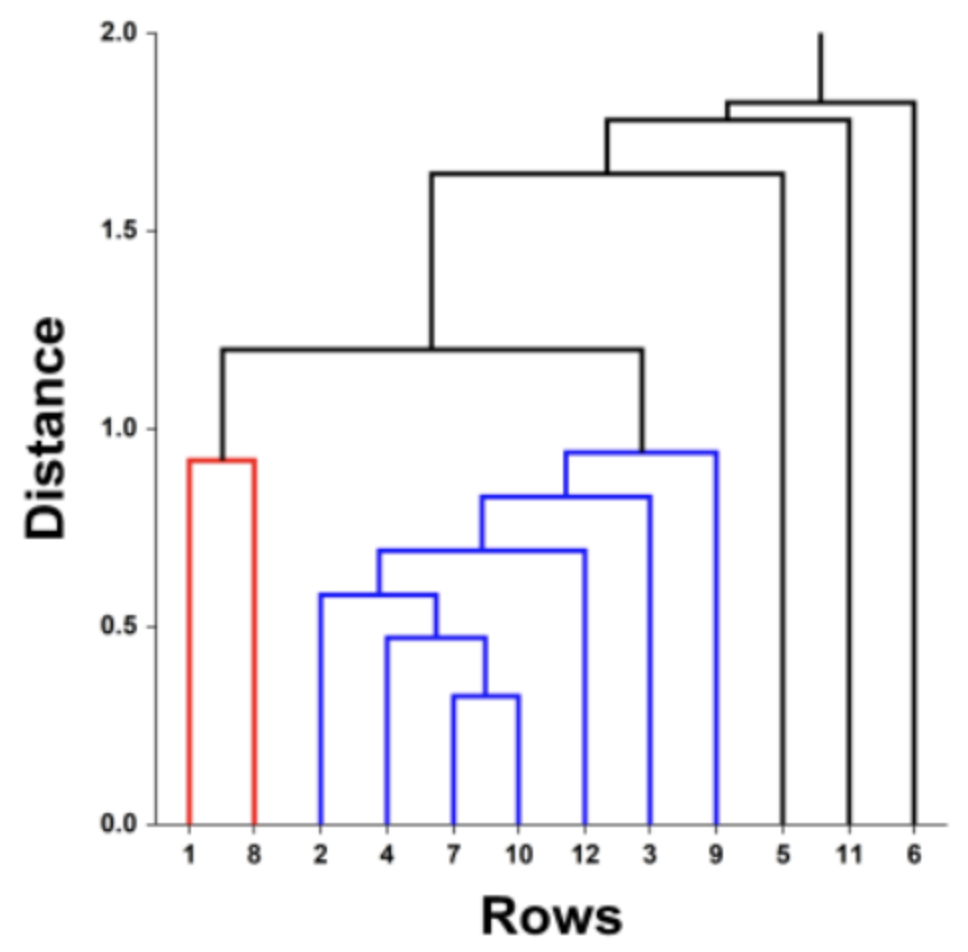
\includegraphics[keepaspectratio,scale=0.5]{chapter5_images/dendogram_distance_example.png}
\caption{Toy Dendogram example}
\label{dendogram_example}
\end{figure*}

The number of clusters that would be formed at a particular cutoff can be easily determined in Figure \ref{dendogram_example} by drawing a horizontal line at that value in the $y$ axis and counting the number of lines that horizontal line intersects. For instance, one line drawn at distance 1.5 would split the data into 4 different clusters. One way to obtain the optimal number of clusters is by drawing the cutoff line at the segment that contains the biggest distance, which is this case happens to be under the segment where 1.5 is.

In order to reach good results, the use of both techniques (Silhouette Coefficient and Dendogram) or even others available in the literature is recommended to find the best number of clusters. It is also recommended to perform an exploratory analysis in the resulting set of clusters, firstly to check if all clusters contain a reasonable amount of data points, otherwise they won't be representative. Then, if the clusters are representative, then take the average and other descriptive statistic metric from the dimensions clustered with the goal of understanding if the cluster distributions reveal multidimensional similarities between the data points or if they seem to have no reason for being grouped. If interpreting the result is hard, then maybe the chosen number of clusters isn't optimal or the algorithm may not be the best tool to segment the dataset. 

\subsubsection{Models and error classes}

To perform this experiment, all the 15 sentences extracted to match each one of the 4 complexities were labelled with binary columns that indicate the absence or presence of one error class. Every one of the 4 models had 60 sentences representing them, totalling 240. The original dataset contains one column for each type of error, along with columns that represent the models used and columns that represent the complexity to which each sentence was classified. However, to simplify our analysis, we have split the results of the same experiment into 2 pairs of interest: models compared to error classes and sentence complexity compared to error classes. In this section, the former one will be presented.

\begin{figure*}[h]
\centering 
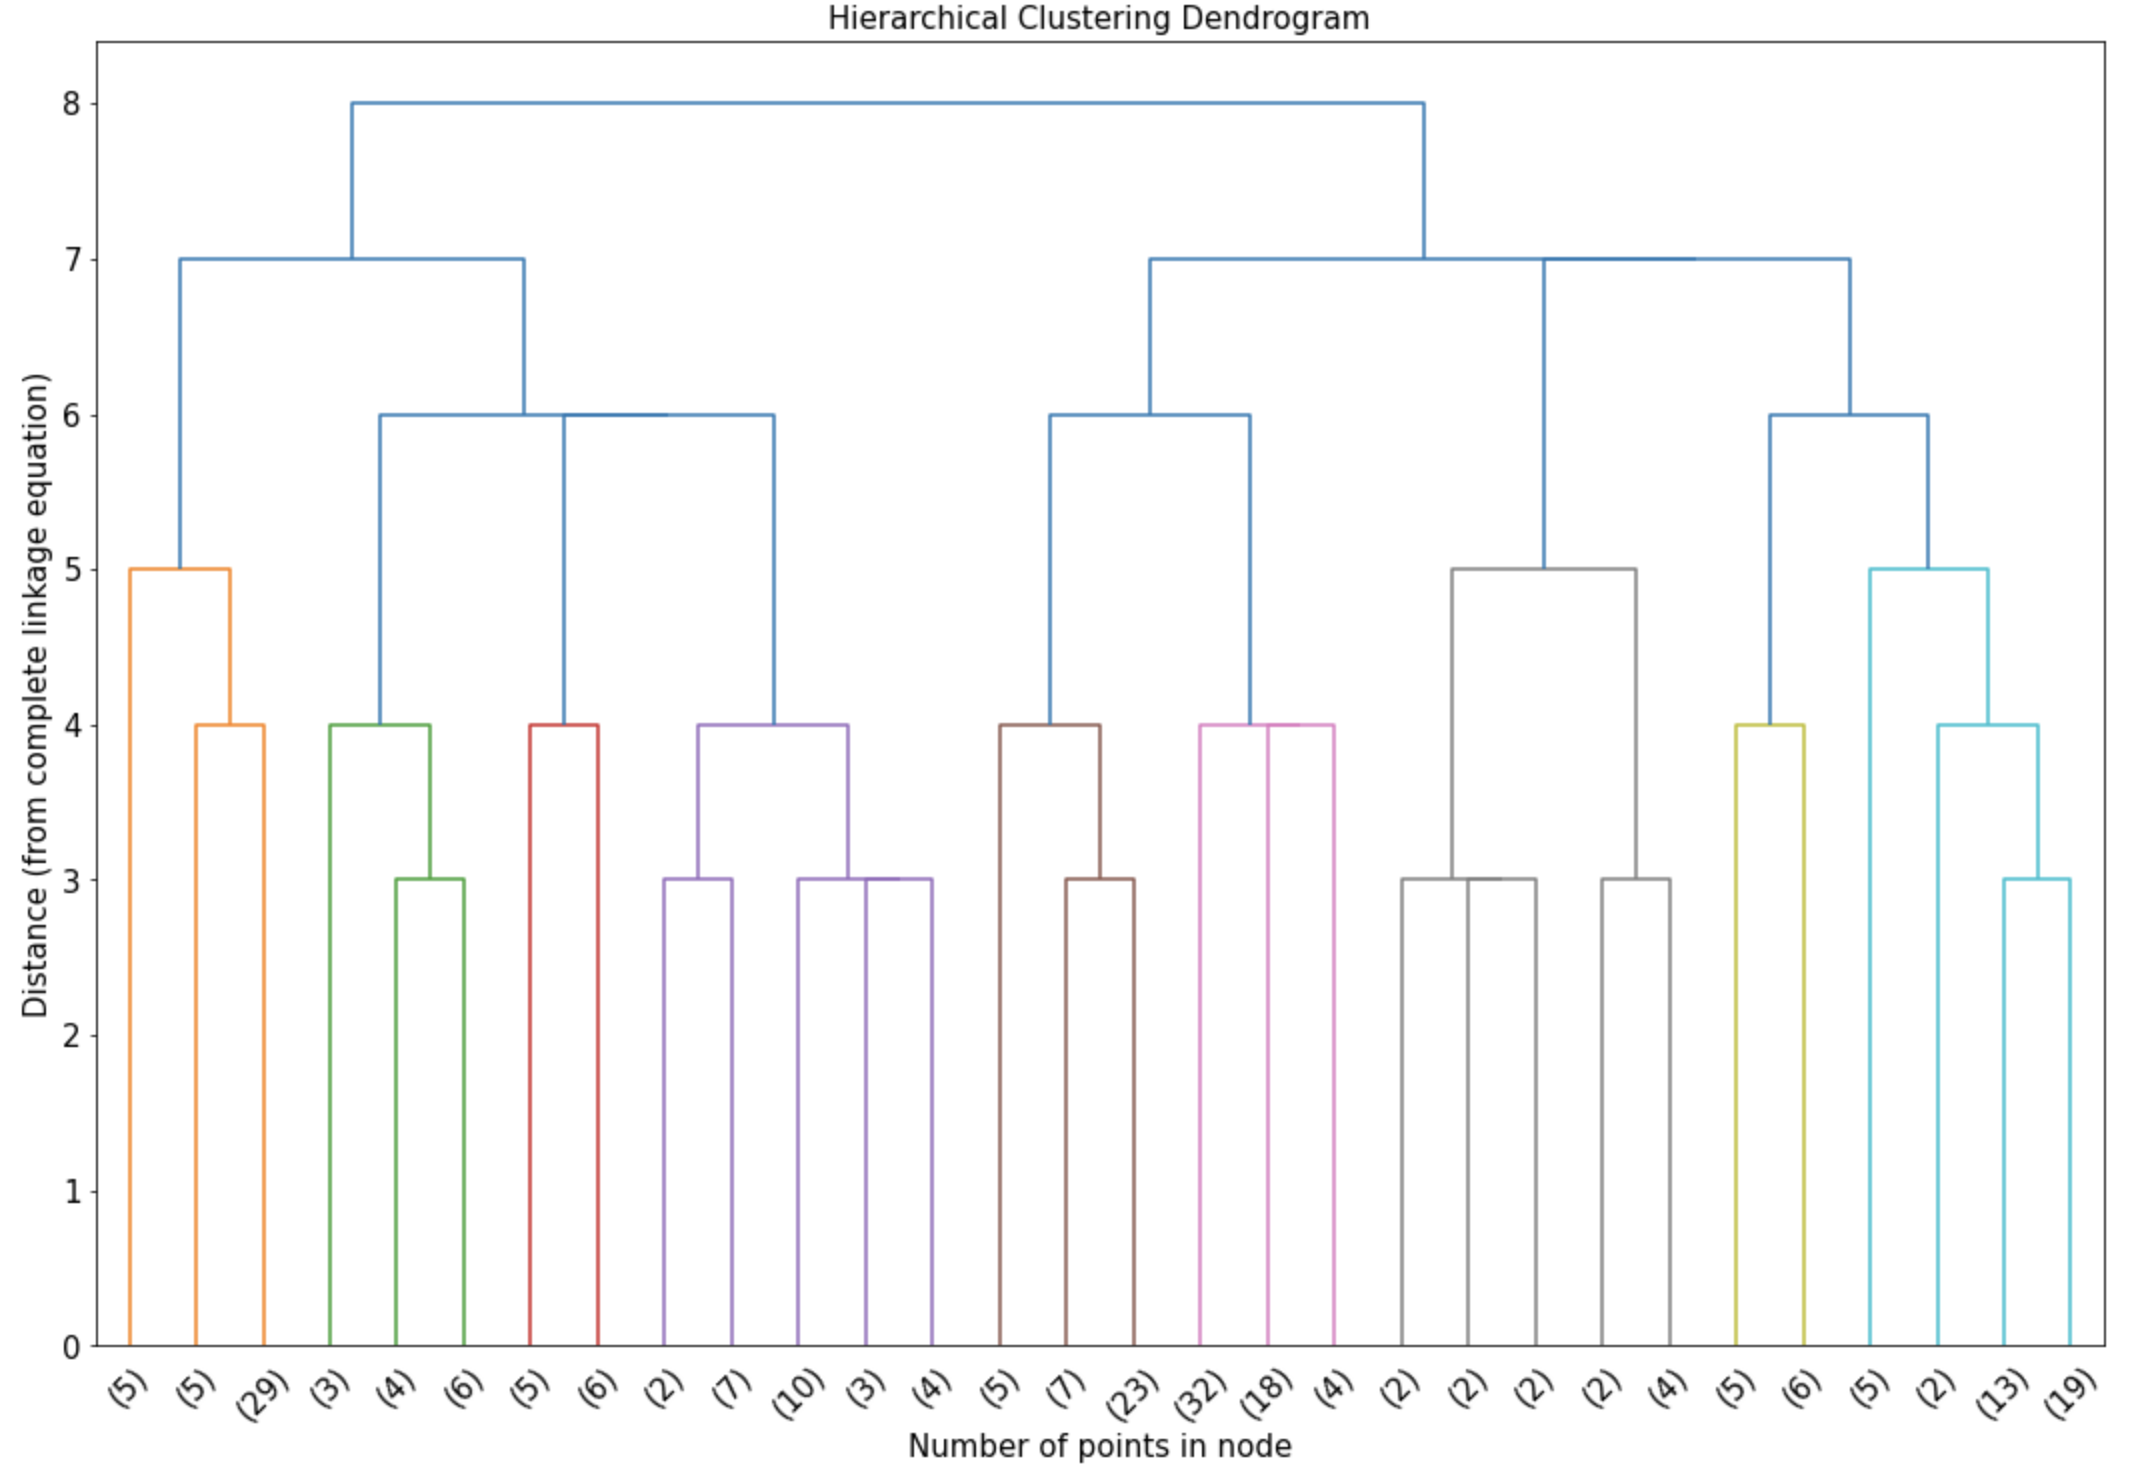
\includegraphics[keepaspectratio,scale=0.4]{chapter5_images/hc_dendogram.png}
\caption{Dendogram of Hierarchical Clustering experiments}
\label{hc_dendogram}
\end{figure*}

Hierarchical Clustering has been applied to the dataset using the manhattan distance, which is appropriate for categorical data, that happens to be the case here since the columns representing the error classes are binary. The Linkage parameter has been chosen after running some experiments with different linkage types and numbers of clusters, with the goal of understanding better how the clusters were formed. The complete linkage approach was chosen since the other ones that are applicable using the manhattan distance had many clusters representing few data points, an issue that could potentially hinder our analysis. 

After choosing the complete linkage, the next step was to compute the whole Dendogram, which can be seen in Figure \ref{hc_dendogram}. The Dendogram has been truncated and as a consequence it grouped some of the data points, otherwise it would be hard to understand the lineage of merges and the cluster groups. Inspecting the graph induces the reader to a doubt regarding where to put the cutoff, since the distances are more or less the same for each cluster group. This is a consequence of using categorical data, it looks like the distances are binned and the number of clusters could not be inferred by graphical inspection in this case. Despite such limitations, there seem to have some option such as 2, 5 and 9 clusters.

Since using the Dendogram for determining the number of cluster didn't work, the silhouette coefficient has been calculated for some linkage approaches and a set of different clusters ranging from 3 to 10. The resulting coefficients are arranged in Table \ref{silhouette_results}. The group average linkage coefficients are shown just for comparison, since it didn't make sense to use them as they created disproportionate cluster groups where some clusters represent a few points and others contain the majority of the dataset. 

\begin{table}[h]
  \caption{Silhouette coefficients per linkage approach and number of clusters}
  \label{silhouette_results}
  \centering
  {\footnotesize
  \begin{tabular}{| p{2.5cm} | P{2.0cm} | P{2.0cm} |}
    \hline
    Linkage & Number of clusters & Silhouette coefficient \\
    \hline
    Complete & 3 & 0.1415 \\
    \hline
    Complete & 4 & 0.1442 \\
    \hline
    Complete & 5 & \textbf{0.2320} \\
    \hline
    Complete & 6 & 0.2199 \\
    \hline
    Complete & 7 & 0.2368 \\
    \hline
    Complete & 8 & 0.2665 \\
    \hline
    Complete & 9 & 0.2931 \\
    \hline
    Complete & 10 & 0.2930 \\
    \hline
    Group Average & 2 & 0.3449 \\
    \hline
    Group Average & 3 & 0.2659 \\
    \hline
    Group Average & 4 & 0.2349 \\
    \hline
\end{tabular}}
\end{table}

Considering the coefficients of Table \ref{silhouette_results} and also calculating the amount of sentences per cluster, we concluded that the most appropriate setup was the one using complete linkage and 5 clusters. If the number of clusters was increased, the complexity of interpreting the results also increases significantly, without a great compensation on the coefficient side. For instance, using 10 clusters would lead to an increase of only $0.061$ points (about 26\%) with a substantial increase in complexity when performing the analysis, while using 7 clusters would lead to an increase of $0.048$ (about 2\%). On the other hand, when choosing a smaller number of clusters such as 3, the decrease in the coefficient would be of $0.0905$ (about 39\%), which is a penalizing trade-off.

After fixing the amount of clusters and setting the experiment configuration, some descriptive metrics were generated for each cluster to help understand how the dataset has been segmented: the average incidence of errors among all error classes, the average occurrence of errors per error class and the share of sentences that belong to each of the models. All these metrics are exposed in Table \ref{error_model_incidence}.

\begin{table}[h]
  \caption{Prevalence of error classes and models per cluster}
  \label{error_model_incidence}
  \centering
  {\footnotesize
  \begin{tabular}{| p{2.0cm} | P{3.5cm} | P{1.2cm} | P{1.2cm} | P{1.2cm} | P{1.2cm} | P{1.2cm} |}
    \hline
    Dimension Name & Dimension Value & Cluster 0 & Cluster 1 & Cluster 2 & Cluster 3 & Cluster 4 \\
    \hline
    \multirow{8}{2.0cm}{Error class} & Reference Matching & 86\% & 74\% & 97.75\% & 41.67\% & 0\% \\
    \cline{2-7}
    & Omission & 46\% & 58\% & 48.31\% & 75\% & 20.51\% \\
    \cline{2-7}
    & Out of Context & 16\% & 2\% & 17.98\% & 100\% & 12.82\% \\
    \cline{2-7}
    & Verb Tense & 98\% & 52\% & 1\% & 58.33\% & 2.56\% \\
    \cline{2-7}
    & Meaning Deviation & 18\% & 62\% & 29.21\% & 91.67\% & 15.38\% \\
    \cline{2-7}
    & Insertion & 26\% & 72\% & 23.6\% & 50\% & 23.08\% \\
    \cline{2-7}
    & Repetition & 12\% & 40\% & 2.23\% & 8.33\% & 10.25\% \\
    \cline{2-7}
    & $<$unk$>$ & 2\% & 80\% & 14.6\% & 16.67\% & 2.56\% \\
    \hline
    \multirow{4}{2.0cm}{Model Name} & 33\% TED Transformer & 22\% & 30\% & 23.60\% & 33.33\% & 23.08\% \\
    \cline{2-7}
    & 66\% TED Transformer & 22\% & 38\% & 20.22\% & 16.67\% & 25.64\% \\
    \cline{2-7}
    & BPE Transformer & 34\% & 4\% & 26.97\% & 41.67\% & 30.77\% \\
    \cline{2-7}
    & BT Transformer & 22\% & 28\% & 29.21\% & 8.33\% & 20.51\% \\
    \hline
    \hline
    \multicolumn{2}{|c|}{Average error incidence among all classes} & 38\% & 55\% & 29.35\% & 55.21\% & 10.9\% \\
    \hline
    \multicolumn{2}{|c|}{Amount of sentences} & 50 & 50 & 89 & 12 & 39 \\
    \hline
\end{tabular}}
\end{table}

To complement the overall descriptive statistics derived from the cluster analysis, we have also generated a Table that contains all the types of errors in each cluster that a model has made, considering only those that reached a higher incidence than 50\% of all their sentences in that cluster. The error class for all models are shown if at least one model has performed the error for more than 50\% of its sentences. The goal of this analysis is to highlight the strongest associations between error classes and models, reduce subjectivity and reach more feasible conclusions. This relation is available in Table \ref{cluster_ranking_model_error}.

\begin{table}[t!]
  \caption{Rank of most frequent errors per model in each cluster}
  \label{cluster_ranking_model_error}
  \centering
  {\footnotesize
  \begin{tabular}{| p{3.2cm} | P{1.4cm} | P{1.8cm} | P{3.5cm} | P{0.9cm} | P{1.3cm} |}
    \hline
                   Error class &     Value &        Sentences &                    Model Name &  Rank &  Cluster \\
    \hline
         Verb tense  &  1.0000 &             11 &           33\% TED Transformer &     1 &        0 \\
    \hline
         Verb tense  &  1.0000 &             11 &           66\% TED Transformer &     2 &        0 \\
    \hline
         Verb tense  &  1.0000 &             17 &               BPE Transformer &     3 &        0 \\
    \hline
         Verb tense  &  0.9090 &             11 &                 BT Transformer &     4 &        0 \\
    \hline
 Reference matching  &  0.9090 &             11 &           33\% TED Transformer &     1 &        0 \\
    \hline
 Reference matching  &  0.8181 &             11 &           66\% TED Transformer &     3 &        0 \\
 \hline
 Reference matching  &  0.8823 &             17 &               BPE Transformer &     2 &        0 \\
 \hline
 Reference matching  &  0.8181 &             11 &                 BT Transformer &     4 &        0 \\
 \hline
          Insertion  &  0.8666 &             15 &           33\% TED Transformer &     2 &        1 \\
          \hline
          Insertion  &  0.6842 &             19 &           66\% TED Transformer &     3 &        1 \\
          \hline
          Insertion  &  1.0000 &              2 &               BPE Transformer &     1 &        1 \\
          \hline
          Insertion  &  0.5714 &             14 &                 BT Transformer &     4 &        1 \\
          \hline
         Verb tense  &  0.4000 &             15 &           33\% TED Transformer &     3 &        1 \\
         \hline
         Verb tense  &  0.3684 &             19 &           66\% TED Transformer &     4 &        1 \\
         \hline
         Verb tense  &  1.0000 &              2 &               BPE Transformer &     1 &        1 \\
         \hline
         Verb tense  &  0.7857 &             14 &                 BT Transformer &     2 &        1 \\
         \hline
  Meaning deviation  &  0.8666 &             15 &           33\% TED Transformer &     2 &        1 \\
  \hline
  Meaning deviation  &  0.5263 &             19 &           66\% TED Transformer &     3 &        1 \\
  \hline
  Meaning deviation  &  1.0000 &              2 &               BPE Transformer &     1 &        1 \\
  \hline
  Meaning deviation  &  0.4285 &             14 &                 BT Transformer &     4 &        1 \\
  \hline
              <unk>  &  0.8666 &             15 &           33\% TED Transformer &     1 &        1 \\
              \hline
              <unk>  &  0.7894 &             19 &           66\% TED Transformer &     3 &        1 \\
              \hline
              <unk>  &  0.0000 &              2 &               BPE Transformer &     4 &        1 \\
              \hline
              <unk>  &  0.8571 &             14 &                 BT Transformer &     2 &        1 \\
              \hline
           Omission  &  0.6000 &             15 &           33\% TED Transformer &     2 &        1 \\
           \hline
           Omission  &  0.5263 &             19 &           66\% TED Transformer &     3 &        1 \\
           \hline
           Omission  &  0.5000 &              2 &               BPE Transformer &     4 &        1 \\
           \hline
           Omission  &  0.6428 &             14 &                 BT Transformer &     1 &        1 \\
           \hline
 Reference matching  &  0.6000 &             15  &           33\% TED Transformer &     4 &        1 \\
 \hline
 Reference matching  &  0.6842 &             19  &           66\% TED Transformer &     3 &        1 \\
 \hline
 Reference matching  &  1.0000 &              2  &               BPE Transformer &     1 &        1 \\
 \hline
 Reference matching  &  0.9285 &             14  &                 BT Transformer &     2 &        1 \\
 \hline
 Reference matching  &  0.9523 &             21  &           33\% TED Transformer &     4 &        2 \\
 \hline
 Reference matching  &  1.0000 &             18  &           66\% TED Transformer &     1 &        2 \\
 \hline
 Reference matching  &  1.0000 &             24  &               BPE Transformer &     2 &        2 \\
 \hline
 Reference matching  &  0.9615 &             26  &                 BT Transformer &     3 &        2 \\
 \hline
  Meaning deviation  &  1.0000 &              4  &           33\% TED Transformer &     1 &        3 \\
  \hline
  Meaning deviation  &  1.0000 &              2  &           66\% TED Transformer &     2 &        3 \\
  \hline
  Meaning deviation  &  1.0000 &              5  &               BPE Transformer &     3 &        3 \\
  \hline
  Meaning deviation  &  0.0000 &              1  &                 BT Transformer &     4 &        3 \\
  \hline
          Omission  &  1.0000 &              4 &           33\% TED Transformer &     1 &        3 \\
          \hline
          Omission  &  0.5000 &              2 &           66\% TED Transformer &     4 &        3 \\
          \hline
          Omission  &  0.6000 &              5 &               BPE Transformer &     3 &        3 \\
          \hline
          Omission  &  1.0000 &              1 &                 BT Transformer &     2 &        3 \\
          \hline
         Verb tense  &  1.0000 &              4 &           33\% TED Transformer &     1 &        3 \\
         \hline
         Verb tense  &  0.5000 &              2 &           66\% TED Transformer &     2 &        3 \\
         \hline
         Verb tense  &  0.4000 &              5 &               BPE Transformer &     3 &        3 \\
         \hline
         Verb tense  &  0.0000 &              1 &                 BT Transformer &     4 &        3 \\
         \hline
     Out of context  &  1.0000 &              4 &           33\% TED Transformer &     1 &        3 \\
     \hline
     Out of context  &  1.0000 &              2 &           66\% TED Transformer &     2 &        3 \\
     \hline
     Out of context  &  1.0000 &              5 &               BPE Transformer &     3 &        3 \\
     \hline
     Out of context  &  1.0000 &              1 &                 BT Transformer &     4 &        3 \\
     \hline
\end{tabular}}
\end{table}

Although the cluster highlights and the ranking of error class incidence per model are interesting, it doesn't make sense to stop here since the experiment aims to interpret qualitatively the multidimensional relationships. In the bullet points below, statements and conclusions about the data previously presented in the tables are made. They aim to clarify some of the relationships that the algorithm helped to spot:

\begin{enumerate}
    \item Cluster 0: This cluster contains 50 sentences (20.8\% of the total). BPE has the biggest share of sentences (34\%), with the other models having 22\% each. The average occurrence of errors is 38\%, ranking 3rd place (exactly in the middle) when compared to the others. Verb Tense and Reference Matching stand out with an occurrence of 98\% and 86\% respectively, with the least frequent errors being $<$unk$>$ and Repetition with 2\% and 12\% each.
    
    It seems that cluster 0 is biased towards BPE due to its higher share, and it also concentrates the sentences with the highest occurrence of Verb Tense and Reference Matching, since all models made these errors in more than 80\% of their sentences. There are signals that these errors are quite horizontal and common to all models, specially to the dominant model (BPE). This cluster also has the lowest occurrence of the $<$unk$>$ error, which is compatible with the fact that BPE dominates this cluster, since the model is immune to this error.
    
    \item Cluster 1: It contains 50 sentences (20.8\% of the total). The 66\% Transformer has the highest share of sentences (38\%), followed by the 33\% Transformer with 30\%, BT with 28\% and BPE with 4\% (2 sentences). The average occurrence of errors is 55\%, ranking 2nd place with respect to the rest. The $<$unk$>$ (80\%), Reference Matching (74\%) and Insertion (72\%) errors stand out as the most frequent from the rest, while Out of Context error almost didn't happen (2\%) and Repetition (40\%) are the least occurring ones.
    
    Although this is the cluster with the second highest incidence of errors, the gap is narrow (0.21\%) when compared to the first place. It has a strong participation (68\%) of the Transformers trained on a reduced dataset (33\% and 66\%), with BPE and BT occupying less than a third, hence can tell that it is mostly represented by the former models. These 2 dominating models demonstrate a high occurence of Insertion, Meaning Deviation and $<$unk$>$ errors, losing to BT in the ranking when talking of Omission and Verb Tense. This cluster's error distribution difference to the first one are clear: it has the highest occurrence of the Repetition error and the incidence of the $<$unk$>$ error is much more expressive. The main characteristic that sets them apart is that in the first cluster BPE predominates. These distinct error distributions indicate a different bias for such models, which corroborates the hypothesis that the technique indeed has an impact on the translation behaviour. 
    
    \item Cluster 2: Its the biggest cluster with 89 sentences (37\% of the total). The models share almost the same quantity of sentences, with BT and BPE Transformers being the most occurring (29\% and 27\%) while the others have about the same slice of the rest. The average frequency of errors is 29\%, being the second with less mistakes. Reference Matching is almost ubiquitous (98\%), whereas curiously the other errors have all less than 50\% of occurrence. Verb Tense and Repetition almost don't happen with 2\% and 1\% respectively.
    
    The most representative cluster is also fairly equally distributed, and the high incidence of Reference Matching in this sample, ranging from 95.23\% to 100\% in the ranking, indicates that this is an error that these models can hardly avoid. In fact, this error is the most common among all the clusters and in the original dataset. It is known to be a flaw of the translation process and probably it can only be addressed by modifying the methodology (such as using references from several human translators), not by the technique or the model. Moreover, this cluster basically tells that in most of the dataset, the models do not perform the Verb Tense or the Repetition errors, but as their incidence varies a lot from cluster to cluster, we cannot claim this as a rule as they happen to other sentences.
    
    \item Cluster 3: It is a small cluster with 12 errors (5\% of the total), with BPE having the most sentences (42\%), followed by the 33\% Transformer (33\%) and a very small contribution from BT (8\%). The average frequency of errors is the highest, with 55.2\%, where Out of Context error is unanimous (100\%), followed by Meaning Deviation (92\%) and Omission (75\%). The least frequent errors are Repetition (8\%) and $<$unk$>$ (16\%).
    
    This cluster has a small share of the total sentences, but concentrates the ones that were the most difficult for all models, curiously with a higher share belonging to BPE. The errors that stood out in this cluster deviating from the share of the others were the Meaning Deviation error (91.67\% vs 42.85\% on average), Out of Context (100\% vs 29.76\% on average) and Omission (75\% vs 49.56\%). Anticipating one result of the complexity section, this cluster has about 75\% of its sentences belonging to B2 and B1, while the others had a lower share (from 66\% to 7.6\%) in these higher complexities, which explains the high error metrics here. The share of errors in this cluster doesn't weight much in the overall bias of the original models as it contains only 5\% of all sentences, hence its sample reduces the relevance of conclusions derived from interpreting its distribution.
    
    \item Cluster 4: A medium-sized 39 error cluster, encompassing the rest of the dataset with 16\% of the total. The BPE Transformer is the most influential contributing with 30\% of the sentences, while the rest is approximately equally distributed among the rest, with BT being the weakest (20.5\%). Errors have spawned the least in this cluster (10.9\%), with no errors occurring more than 50\% of the sentences. Insertion is the most frequent one (23\%), while Reference Matching does not happen at all, followed by $<$unk$>$ and Verb Tense, both with 2\%.
    
    This cluster contrasts with the last one as its low occurrence of errors happens as a result of the lower complexity of its sentences, with 84.6\% being A1. This may explain why no errors happen in more than 50\% of sentences and its low average incidence of errors. Regarding the scarcity of errors, the error classes that drive more attention are Reference Matching (0\% vs 59.88\% on average), Verb Tense (2.56\% vs 42.38 on average) and $<$unk$>$ (2.56\% vs 23.17\% on average).
\end{enumerate}

The results reported for this experiment attempt to elaborate qualitative hypothesis that justify the distributions and biases shown for each model. Despite the sample limitations and constraints established by the error classes created, it sheds some light on the impact that each technique has into the errors made by the model. There is some evidence that the reduced models tend to perform the Repetition and $<$unk$>$ errors, which may be associated with a lack of vocabulary sort of bias. Errors like Reference Matching seem to happen independently of the technique and Verb Tense is also horizontal, but usually more common when BPE is responsible for most sentences. Whenever the Transformers trained on reduced TED 33\% and 66\% appear, their share of sentences in a cluster tends to be the same, which can be an evidence that the algorithm sees some correlation between their error patterns. Also, curiously, whenever the Meaning Deviation error is present, the BT Transformer has the lowest occurrence, and it is also less present in clusters where BT has a higher share.

Some results already anticipated comparisons with the complexity analysis to provide a deeper understanding of the characteristics of each cluster, but the reader is still encouraged to go through the whole complexity analysis that will be presented in the next section. 

\subsubsection{Sentence complexity and error classes}

The same analysis and rationale presented in the last section applies to this experiment, the difference is that before we had ignored the presence of complexity as a dimension, but now we do this for the model variants and focus on relating complexity with error classes. Therefore, the qualitative results presented here had the same silhouette coefficient (0.2320) and used the same amount of clusters (5). 

To gain a better understanding of the distribution of each cluster, descriptive metrics such as the average incidence of errors among all error
classes, the average and median occurrence of errors per error class and the share of sentences that belong to each complexity type have been generated and are exposed in Table \ref{error_complexity_incidence}. The main difference between Tables \ref{error_complexity_incidence} and \ref{error_model_incidence} are the last 4 rows that show the complexity share in each cluster rather than model share. 

\begin{table}[h]
  \caption{Error class and complexity incidence per cluster}
  \label{error_complexity_incidence}
  \centering
  {\footnotesize
  \begin{tabular}{| p{2.0cm} | P{3.5cm} | P{1.2cm} | P{1.2cm} | P{1.2cm} | P{1.2cm} | P{1.2cm} |}
    \hline
    Dimension Name & Dimension Value & Cluster 0 & Cluster 1 & Cluster 2 & Cluster 3 & Cluster 4 \\
    \hline
    \multirow{8}{2.0cm}{Error class} & Reference Matching & 86\% & 74\% & 97.75\% & 41.67\% & 0\% \\
    \cline{2-7}
    & Omission & 46\% & 58\% & 48.31\% & 75\% & 20.51\% \\
    \cline{2-7}
    & Out of Context & 16\% & 2\% & 17.98\% & 100\% & 12.82\% \\
    \cline{2-7}
    & Verb Tense & 98\% & 52\% & 1\% & 58.33\% & 2.56\% \\
    \cline{2-7}
    & Meaning Deviation & 18\% & 62\% & 29.21\% & 91.67\% & 15.38\% \\
    \cline{2-7}
    & Insertion & 26\% & 72\% & 23.6\% & 50\% & 23.08\% \\
    \cline{2-7}
    & Repetition & 12\% & 40\% & 2.23\% & 8.33\% & 10.25\% \\
    \cline{2-7}
    & $<$unk$>$ & 2\% & 80\% & 14.6\% & 16.67\% & 2.56\% \\
    \hline
    \multirow{4}{2.0cm}{CEFR Complexity} & A1 & 4\% & 16\% & 19.10\% & 0\% & 84.62\% \\
    \cline{2-7}
    & A2 & 32\% & 20\% & 31.46\% & 25\% & 7.69\% \\
    \cline{2-7}
    & B1 & 42\% & 8\% & 32.58\% & 25\% & 7.69\% \\
    \cline{2-7}
    & B2 & 22\% & 56\% & 16.85\% & 50\% & 0\% \\
    \hline
    \hline
    \multicolumn{2}{|c|}{Average error incidence among all classes} & 38\% & 55\% & 29.35\% & 55.21\% & 10.9\% \\
    \hline
    \multicolumn{2}{|c|}{Amount of sentences} & 50 & 50 & 89 & 12 & 39 \\
    \hline
\end{tabular}}
\end{table}

As this experiment has an intersection of results with the last one, since the error class distribution is the same, the relations described here will be more concise to avoid redundancy when comparing to the results already reported. Looking at the distributions of sentece complexity per cluster, a first look indicates that the average error incidence is somewhat correlated to which complexity dominates in that cluster. The correlation between the error incidence and the share of complex sentencees (considering B1 and B2) reached 0.9248, which indicate that the segmentation performed is somewhat accurate and there is a strong evidence that the complexity also influences the categories of error that happen.

Analogously to the analysis performed in the model-error section, a ranking of the complexities per cluster that had at least one error class with more than 50\% of occurrence has also been generated and is available in Table \ref{cluster_ranking_complexity_error}. The data exhibited in this table will be commented for each cluster to with the goal of extracting qualitative conclusions: 

\begin{table}[t!]
  \caption{Rank of most frequent errors per complexity in each cluster}
  \label{cluster_ranking_complexity_error}
  \centering
  {\footnotesize
  \begin{tabular}{| p{3.2cm} | P{1.4cm} | P{1.8cm} | P{3.5cm} | P{0.9cm} | P{1.3cm} |}
         \hline
         Error class         &     Value &        Sentences &                    Complexity &  Rank &  Cluster \\
         \hline
         Reference matching  &  1.0000 &             11 &         B2 &     1 &        0 \\
         \hline
         Reference matching  &  0.8750 &             16 &         A2 &     2 &        0 \\
         \hline
         Reference matching  &  0.8571 &             21 &         B1 &     3 &        0 \\
         \hline
         Reference matching  &  0.0000 &              2 &         A1 &     4 &        0 \\
         \hline
         Verb tense         &  1.0000 &              2 &         A1 &     1 &        0 \\
         \hline
         Verb tense         &  1.0000 &             21 &         B1 &     2 &        0 \\
         \hline
         Verb tense         &  1.0000 &             11 &         B2 &     3 &        0 \\
         \hline
         Verb tense         &  0.9375 &             16 &         A2 &     4 &        0 \\
         \hline
          $<$unk$>$             &  1.0000 &              4 &         B1 &     1 &        1 \\
          \hline
          $<$unk$>$             &  0.9000 &             10 &         A2 &     2 &        1 \\
          \hline
          $<$unk$>$             &  0.7500 &              8 &         A1 &     3 &        1 \\
          \hline
          $<$unk$>$             &  0.7500 &             28 &         B2 &     4 &        1 \\
          \hline
          Insertion         &  0.8000 &             10 &         A2 &     1 &        1 \\
          \hline
          Insertion         &  0.7500 &              4 &         B1 &     2 &        1 \\
          \hline
          Insertion         &  0.7143 &             28 &         B2 &     3 &        1 \\
          \hline
          Insertion         &  0.6250 &              8 &         A1 &     4 &        1 \\
          \hline
          Meaning deviation  &  0.6786 &             28 &         B2 &     1 &        1 \\
          \hline
          Meaning deviation  &  0.6000 &             10 &         A2 &     2 &        1 \\
          \hline
          Meaning deviation  &  0.5000 &              8 &         A1 &     3 &        1 \\
          \hline
          Meaning deviation  &  0.5000 &              4 &         B1 &     4 &        1 \\
          \hline
           Omission         &  0.8214 &             28 &         B2 &     1 &        1 \\
           \hline
           Omission         &  0.5000 &              4 &         B1 &     2 &        1 \\
           \hline
           Omission         &  0.3000 &             10 &         A2 &     3 &        1 \\
           \hline
           Omission         &  0.1250 &              8 &         A1 &     4 &        1 \\
           \hline
         Reference matching  &  1.0000 &              4 &         B1 &     1 &        1 \\
         \hline
         Reference matching  &  0.8929 &             28 &         B2 &     2 &        1 \\
         \hline
         Reference matching  &  0.5000 &              8 &         A1 &     3 &        1 \\
         \hline
         Reference matching  &  0.4000 &             10 &         A2 &     4 &        1 \\
         \hline
         Verb tense         &  0.8214 &             28 &         B2 &     1 &        1 \\
         \hline
         Verb tense         &  0.5000 &              4 &         B1 &     2 &        1 \\
         \hline
         Verb tense         &  0.1250 &              8 &         A1 &     3 &        1 \\
         \hline
         Verb tense         &  0.0000 &             10 &         A2 &     4 &        1 \\
         \hline
         Reference matching  &  1.0000 &             28 &         A2 &     1 &        2 \\
         \hline
         Reference matching  &  1.0000 &             15 &         B2 &     2 &        2 \\
         \hline
         Reference matching  &  0.9655 &             29 &         B1 &     3 &        2 \\
         \hline
         Reference matching  &  0.9412 &             17 &         A1 &     4 &        2 \\
         \hline
          Meaning deviation  &  1.0000 &              3 &         A2 &     1 &        3 \\
          \hline
          Meaning deviation  &  1.0000 &              6 &         B2 &     2 &        3 \\
          \hline
          Meaning deviation  &  0.6667 &              3 &         B1 &     3 &        3 \\
          \hline
           Omission         &  1.0000 &              3 &         B1 &     1 &        3 \\
           \hline
           Omission         &  0.8333 &              6 &         B2 &     2 &        3 \\
           \hline
           Omission         &  0.3333 &              3 &         A2 &     3 &        3 \\
           \hline
         Out of context     &  1.0000 &              3 &         A2 &     1 &        3 \\
         \hline
         Out of context     &  1.0000 &              3 &         B1 &     2 &        3 \\
         \hline
         Out of context     &  1.0000 &              6 &         B2 &     3 &        3 \\
         \hline
         Verb tense         &  0.8333 &              6 &         B2 &     1 &        3 \\
         \hline
         Verb tense         &  0.6667 &              3 &         B1 &     2 &        3 \\
         \hline
         Verb tense         &  0.0000 &              3 &         A2 &     3 &        3 \\
         \hline
\end{tabular}}
\end{table}

\begin{enumerate}
    \item Cluster 0: It is mostly allocated with sentences belonging to higher complexities (66\% of B1 and B2), with only 4\% belonging to A1. The presence of high complexities makes sense given the average incidence of errors to be about 38\% (which could be an even higher amount). Curiously, the Reference Matching error has no occurrence in A1 sentences, while the other complexities push its average to higher levels as they are all greater than 85\%. Regarding the Verb Tense error, which is another one that has a high incidence in this cluster, it seems that its average is uncorrelated to the sentence complexities.
    \item Cluster 1: This cluster has a similar allocation to higher complexities (64\% of B1 and B2), a bit similar to the previous cluster, but with a higher share allocated to A1 (16\%). It has the second highest error average of errors per sentence (55\%), much higher than cluster 1, even though it has a similar complexity distribution. A look in the rank tells that error classes do not change their average occurrence proportionally to the complexity share of sentences, such as $<$unk$>$ and Insertion. This conclusion is based on the fact that the average does not follow a monotonic trend when compared to a gradually increasing complexity, with some of those errors even having a smaller incidence among B2 sentences. Conversely, some errors do attend the approximately monotonic trend, namely Verb Tense, Omission and Meaning Deviation. The other Reference Matching error is somewhat neutral, with half of the complexities achieving expectations and the others not. 
    \item Cluster 2: It's the largest cluster with 89 sentences, with 49\% of them belonging to the more challenging complexities B1 and B2. It has the second smallest error average (29.35\%), as expected smaller than other clusters with higher complexities on average. Only one error had more than 50\% of incidence, and the complexity rank for this error shows that it appears to be a bit uncorrelated to this dimension, since A2 and B2 have the same error average.
    \item Cluster 3: This tiny cluster of 12 sentences has 75\% of them belonging to B2 and B1 complexities, the highest among all, which probably is correlated with the fact that it has the highest error average (55.2\%). Curiously, the HC algorithm has eliminated the A1 complexity of this cluster, which makes sense if the goal was to concentrate the most error prone sentences. Its ranking of most occurring errors per complexity shows some errors that appear to not increase their incidence with an increase in the CEFR dimension, which are Meaning Deviation and Out of Context. On the other hand, Verb Tense and Omission show a relevant difference for A2 and B2 sentences, as expected. 
    \item Cluster 4: The last cluster contains 39 sentences and is the one with the lowest occurrence of errors, about 10.9\%. This is somewhat compatible to the fact that 84.6\% of those sentences are A1 and none belong to B2. There are no errors capable of reaching an occurrence higher than 50\%, so there isn't much to analyse here, it looks like the algorithm preferred to agglomerate easier sentences that are less prone to errors.
\end{enumerate}

Now with complexity, model types and error classes all explored using the most appropriate Hierarchical Clustering parameters, the motivations behind the segmentation performed for each cluster are clearer. The algorithm has agglomerated sentences with similar complexity in some clusters, specially 3 and 4, notwithstanding the fact that it didn't receive this information beforehand. Also, for a significant share of sentences the average error incidence also increases with complexity, which is an evidence that the criteria used to rank the CEFR levels was at some level right. 

The diversity and share of errors also differs a lot from cluster to cluster depending on the sentence complexity share. For instance the Verb Tense errors seem to have some correlation with the difficulty of sentences by looking at Table \ref{cluster_ranking_complexity_error}, except for cluster 0. The same happens for Omission, with no exceptions. Nonetheless, it is hard to separate the influence of complexity or model technique to understand why the final error distribution behaves in some manner, as the influence on it is multidimensional, but there are already some interesting trends outlined that wouldn't be feasible by assessing its performance purely through scores. 
 
\subsection{Correspondence Analysis (CA) experiment} $\abbrev{Correspondence Analysis}{CA}$ 

% https://github.com/MaxHalford/prince#multiple-correspondence-analysis-mca
% https://ce.aut.ac.ir/~shiry/lecture/Advanced%20Machine%20Learning/Manifold_Modern_Multivariate%20Statistical%20Techniques%20-%20Regres.pdf

CA in practice is an exploratory multivariate technique that is capable of processing a N-dimensional table, extract its principal components and generate coordinates for them. These coordinates can be plotted into a N-Dimensional visualization that can help interpret relations between the dimensions. The most common case happens with 2 dimensions, where a co-occurrence matrix is converted into a 2-D visualization, and its rows and columns are depicted as points. The table that contains the dimension occurrences, which is also called contingency matrix, may have 2 dimensions or $N$ dimensions, being called Simple Correspondence Analysis in the former case and Multiple Correspondence Analysis in the latter. 

\subsubsection{Why use CA for qualitative analysis?}

CA is considered to be the Principal Components Analysis (PCA) \abbrev{Principal Components Analysis}{PCA} variant suitable for categorical data, as mentioned in \citet{Greenacre1987TheGI}, which makes it a perfect fit for the purpose of this work. The coordinates generated by the algorithm are analogous to factors in PCA (used for continuous data), but the key difference is that they partition the Chi-square value is used in testing independence instead of the total variance.

This algorithm benefits from the properties of Singular Value Decomposition (SVD) \abbrev{Singular Value Decomposition}{SVD} similarly to how PCA does it. It basically diagonalizes the covariance matrix of the input data, finding the major axes to represent the same distribution with a confidence level that depends on the eigenvalues of the first 2 factors. Given that the algorithm is able to fit the data with a decent explained variance, the resulting visualization enables a geometric interpretation that explains the relations between the variables, made possible also by the use of the Chi-square statistic. The potential to extract relevant relations depends on whether the explained variance is considered to be significant or not. There is no hard rule to describe what is a good explained variance, it depends on the rigor of the analysis. Values above 80\% considering the principal components are considered satisfactory and above 90\% are an almost ideal fit.

The CA algorithm has been applied to the same qualitative dimensions mentioned in the previous experiments (models and error classes or complexities and error classes). Literature shows that the conclusions derived from Simple CA are straightforward to interpret, and assessing its effectiveness and reliability is possible through explained variance. Hence, we believe that is has potential to corroborate and possibly complement the conclusions derived from other experiments.

\subsubsection{Implementation of CA}

Some techniques and properties benefited by CA were already mentioned in the beginning of this section, but the complete theory and calculus motivation behind the CA algorithm goes beyond the scope of this work. For more details the reader is referred to \citet{multivariate-izenman}. In order to gain a better understanding of the \textit{modus operandi} of this algorithm, a step by step pseudocode is provided here, heavily inspired by some course material \cite{ncss_correspondence} and the aforementioned book \cite{multivariate-izenman}. 

A co-occurrence matrix \textbf{K}, also referred to as 2-way contingency matrix in literature, is a matrix whose cells enumerate the co-occurrences of specific row-column combinations. Consider the matrix \textbf{K} of dimensions $r \times s$, where $r$ is the number of rows and $s$ is the number of columns. Each row contains one category of dimension $a$ (error class, for instance), that has $r$ categories in total. The same applied for the columns, that contain $s$ categories of dimension $b$. This matrix is the input for the CA algorithm, that is subjected to the following steps in order to obtain the algorithm's output:

\begin{enumerate}
    \item The first assertion that must be made since its necessary for the algorithm to work is that $\textbf{K} \in \mathbb{Z}^{*(r \times s)}_{+}$, therefore all elements of $\mathbf{K}$ must be non-negative and none of the row or column entries sum up zero
    
    \item Compute the proportion matrix $\textbf{P}=XY^{T}\frac{1}{\sum k}$, by dividing each element of K by the sum of all numbers in \textbf{K}. In mathematical terms: \begin{equation}
    P={p_{ij}}=\frac{k_{ij}}{\sum_{i}\sum_{j}k_{ij}}
    \end{equation}
    The expected format of the table would match the representation of Table \ref{correspondence_input}:
\begin{table}[H]
  \caption{Input Matrix \textbf{P} after normalizing \textbf{K}}
  \label{correspondence_input}
  \centering
  {\footnotesize
  \begin{tabular}{| p{2.3cm} | P{1.0cm} | P{1.0cm} | P{1.0cm} | P{1.0cm} | P{1.0cm} | P{1.0cm} | P{2.0cm} |}
    \hline
    Row Variable & $B_{1}$ & $B_{2}$ & \dotsc & $B_{j}$ & \dotsc & $B_{s}$ & Row Total \\
    \hline
    \hline
    $A_{1}$ &
    $p_{11}$ & 
    $p_{12}$ & 
    \dotsc &
    $p_{1j}$ &
    \dotsc &
    $p_{1s}$ &
    $p_{1+}$ \\
    \hline
    $A_{2}$ &
    $p_{21}$ & 
    $p_{22}$ & 
    \dotsc &
    $p_{2j}$ &
    \dotsc &
    $p_{2s}$ &
    $p_{2+}$ \\
    \hline
    \vdots &
    \vdots & 
    \vdots & 
    \vdots &
    \vdots &
    \vdots &
    \vdots &
    \vdots \\
    \hline
    $A_{i}$ &
    $p_{i1}$ & 
    $p_{i2}$ & 
    \dotsc &
    $p_{ij}$ &
    \dotsc &
    $p_{is}$ &
    $p_{i+}$ \\
    \hline
    \hline
    \vdots &
    \vdots & 
    \vdots & 
    \vdots &
    \vdots &
    \vdots &
    \vdots &
    \vdots \\
    \hline
    $A_{r}$ &
    $p_{r1}$ & 
    $p_{r2}$ & 
    \dotsc &
    $p_{rj}$ &
    \dotsc &
    $p_{rs}$ &
    $p_{r+}$ \\
    \hline
    \hline
    Column Total &
    $p_{+1}$ & 
    $p_{+2}$ & 
    \dotsc &
    $p_{+j}$ &
    \dotsc &
    $p_{+s}$ &
    1 \\
    \hline
\end{tabular}}
\end{table}

    \item The totals of both the rows and columns of \textbf{P} can also be embedded in the vectors \textbf{r} and \textbf{c}, respectively. An accurate representation of these vectors would be 
    
    \begin{equation}
        \textbf{P1}_{s} =
        \begin{bmatrix}
            p_{1+} \\
            \vdots \\
            p_{r+} 
        \end{bmatrix}
        = \textbf{r}
    \end{equation}
    and 
    \begin{equation}
        \textbf{P}^{T}\textbf{1}_{r} =
        \begin{bmatrix}
            p_{+1} \\
            \vdots \\
            p_{+s} 
        \end{bmatrix}
        = \textbf{c},
    \end{equation}
    
    which are also known as average row and column profiles. Consider the generation of matrices $D_{r} = [diag(\textbf{r})]^{-1/2}$ and $D_{c} = [diag(\textbf{c})]^{-1/2}$, that are constituted of a matrix of zeroes whose diagonal are the row totals and columns totals of the previous table, respectively. The elements inside the \textbf{r} and \textbf{c} vectors can also be manipulated to generate the diagonal elements of the square matrices
    \begin{equation}
     \textbf{D}_{r} =
     \begin{bmatrix}
     p_{1+} & 0 & 0 \\
     0 & \ddots & 0 \\
      0 & 0 & p_{r+} 
     \end{bmatrix}
    \end{equation}
    and
    \begin{equation}
     \textbf{D}_{c} = 
     \begin{bmatrix}
     p_{+1} & 0 & 0 \\
     0 & \ddots & 0 \\
     0 & 0 & p_{+s}
     \end{bmatrix},
    \end{equation}
    that contain the row and column totals in their diagonal.
    
    \item After obtaining the matrices $\textbf{D}_{r}$ and $\textbf{D}_{c}$, it becomes possible to calculate $\textbf{P}_{r}$ and $\textbf{P}_{c}$, which represent the row and column profiles of P:
    
    \begin{equation}
        \textbf{P}_{r} = \textbf{D}_{r}^{-1}\textbf{P}
        \begin{bmatrix}
            \textbf{a}_{1}^{T} \\
            \vdots \\
            \textbf{a}_{r}^{T}
        \end{bmatrix}
    \end{equation}
    where 
    \begin{equation}
        \textbf{a}_{i}^{T} =
        \begin{bmatrix}
        \frac{k_{i1}}{k_{i+}}, \dotsc, \frac{k_{is}}{k_{i+}}
        \end{bmatrix}
    \end{equation}
    and
    \begin{equation}
        \textbf{P}_{s} = \textbf{D}_{c}^{-1}\textbf{P}^{T}
        \begin{bmatrix}
            \textbf{b}_{1}^{T} \\
            \vdots \\
            \textbf{b}_{s}^{T}
        \end{bmatrix}
    \end{equation}
    where
    \begin{equation}
        \textbf{b}_{j}^{T} =
        \begin{bmatrix}
        \frac{k_{ij}}{k_{+j}}, \dotsc, \frac{k_{rj}}{k_{+j}}
        \end{bmatrix}.
    \end{equation}
    
    \item In this step, a key insight of the algorithm enables its output to become an interpretable graph, where the distances resemble relationships between the dimensions. Please note that the steps have been summarized, but the most important manipulations were kept. The chi-square distribution is used as a measure of distance to compute the row and column distances, and it is calculated as follows: 
        \begin{itemize}
            \item Row profile distances. Consider $a_{i}$ and $a_{i^{'}}$ that are entries of the row profiles. The squared $\chi^{2}$ distance between them is given by
        \begin{equation}
            d^{2}(\textbf{a}_{i}, \textbf{a}_{i^{'}}) = (\textbf{a}_{i} - \textbf{a}_{i^{'}})^{T}\textbf{D}_{c}^{-1}(\textbf{a}_{i} - \textbf{a}_{i^{'}}) = \sum^{s}_{j=1}\frac{k}{k_{+j}} (\frac{k_{ij}}{k_{i+}} - \frac{k_{i^{'}j}}{k_{i^{'}+}}).
        \end{equation}
        However, the distance that can correlate a dimension category with its corresponding centroid is the most valuable to be represented in the plot. Considering row profiles, their centroids are represented by \textbf{c}. The value of the distance to their centroid can be obtained by  
        \begin{equation}
            d^{2}(\textbf{a}_{i}, \textbf{c}) = (\textbf{a}_{i} - \textbf{c})^{T}\textbf{D}_{c}^{-1}(\textbf{a}_{i} - \textbf{c}) = \frac{1}{k_{i+}} \sum^{s}_{j=1} \frac{k}{k_{i+}k_{+j}} (k_{ij} - \frac{k_{i+}k_{+j}}{k}),
        \end{equation}
        which when summed over all row profiles results in 
        \begin{equation}
        \label{profile_totals}
        k \sum_{i=1}^{r} p_{i+} + d^{2}(a_{i}, c) = \sum_{i=1}^{r} \sum_{j=1}^{s} \frac{(k_{ij} - \frac{k_{i+}k_{+j}}{k})^{2}}{\frac{k_{i+}k_{+j}}{k}},
        \end{equation}
        which is similar to another statistic that we know of. Taking Equation \ref{profile_totals}, and matching $O_{ij}$ with $k_{ij}$ and $E_{ij}$ with $\frac{k_{i+}k_{+j}}{k}$, we find out that it can be approximated with the Pearson's chi-squared statistic, which is
        \begin{equation}
        \label{pearson_statistic}
        X^{2} = \sum_{i} \sum_{j} \frac{(O_{ij} - E_{ij})^{2}}{E_{ij}}.
        \end{equation}
        In Equation \ref{pearson_statistic}, $O_{ij}$ represents the observed cell frequency and $E_{ij}$ the expected cell frequency. The calculation of these terms will be crucial for the next steps.
        
        \item Column profile distances. The reproduction of the steps followed in the row dimension are equivalent for the column dimension, changing only the axis regarding the algebraic manipulations. The column profiles distances can be calculated as
        \begin{equation}
        d^{2}(\textbf{b}_{j}, \textbf{b}_{j^{'}}) = (\textbf{b}_{j} - \textbf{b}_{j^{'}})^{T}\textbf{D}_{r}^{-1}(\textbf{b}_{j} - \textbf{b}_{j^{'}}) = \sum^{r}_{i=1}\frac{k}{k_{i+}} (\frac{k_{ij}}{k_{+j}} - \frac{k_{ij^{'}}}{k_{+j^{'}}}).
        \end{equation}
        Following the same rationale for row profiles, the distance of the column with respect to its centroid is the metric of interest
        \begin{equation}
        d^{2}(\textbf{b}_{j}, \textbf{r}) = (\textbf{b}_{j} - \textbf{r})^{T}\textbf{D}_{r}^{-1}(\textbf{b}_{j} - \textbf{r}) = \frac{1}{k_{+j}} \sum^{r}_{i=1} \frac{k}{k_{i+}k_{+j}} (k_{ij} - \frac{k_{i+}k_{+j}}{k}),
        \end{equation}
        that can analogously be summed over all the column profiles, reaching an Equation that resembles \ref{profile_totals}. Similarly, this resulting equation has structure similarities with the Pearson's chi-squared statistic in Equation \ref{pearson_statistic}.
        \end{itemize}
    
    \item Now we derive the total inertia equation and its decomposition. As we are using dummy categorical variables to represent the dimensions, 
    we proceed with one standard assumption of contingency table analysis where the row and column totals are considered to be fixed and the cell frequencies in \textbf{K} are allowed to vary given those constraints. The relative frequency matrix incorporates such restrictions:
    \begin{equation}
    k^{-1} \textbf{X} (\textbf{I}_{k} - k^{-1}\textbf{J}_{k})\textbf{Y}^{T} = \textbf{P} - \textbf{r}\textbf{c}^{T} = \Tilde{\textbf{P}},
    \end{equation}
    where $K=XY^{T}$, $\textbf{J}_{k}=\textbf{1}_{a}\textbf{1}_{a}^{T}$ is an ($a \times a$)-matrix of 1s and the matrix $\Tilde{\textbf{K}}=k\Tilde{\textbf{P}}$ is also known as the matrix of residuals. This name is given because its $ij$th entry shows the difference between the observed cell frequency $O_{ij}=k_{ij}$ and the expected cell frequency $E_{ij}=\frac{k_{i+}k_{+j}}{k}$, resulting in $\Tilde{k}_{ij}=O_{ij}-E_{ij}$.
    The last step to reach the inertia calculation is to calculate the ($s \times s$)-matrix $\textbf{R}_{0}$
    \begin{equation}
    \textbf{R}_{0} = \textbf{D}_{c}^{\frac{-1}{2}}\Tilde{\textbf{P}}^{T}\textbf{D}_{r}^{-1}\textbf{\Tilde{P}}\textbf{D}_{c}^{\frac{-1}{2}},
    \end{equation}
    where $\textbf{D}_{r}^{-1}=diag\{\textbf{r}^{-1}\}$ and $\textbf{D}_{c}^{\frac{-1}{2}}=diag\{\textbf{c}^{\frac{-1}{2}}\}$. The entry in the $j$th row and $j^{'}$th column of $\textbf{R}_{0}$ is given by
    \begin{equation}
    (k_{+j}k_{+j^{'}})^{\frac{-1}{2}} \sum_{i=1}^{r} \frac{1}{k_{i+}} (k_{ij} - \frac{k_{i+}k_{+j}}{k}) (k_{ij^{'}}-\frac{k_{i+}k_{+j^{'}}}{k})
    \end{equation}
    and the $j$th diagonal entry of $\textbf{R}_{0}$ is obtained by setting $j=j^{'}$,
    \begin{equation}
    \frac{1}{k_{+j}} \sum_{i=1}^{r} \frac{1}{k_{i+}} (k_{ij} - \frac{k_{i+}k_{+j}}{k})^{2}.
    \end{equation}
    The trace of $\textbf{R}_{0}$, which is also the sum of the eigenvalues of $\textbf{R}_{0}$ is 
    \begin{equation}
    \sum_{j=1}^{s} \lambda_{j}^{2} = tr\{\textbf{R}_{0}\} = \sum_{i=1}^{r} \sum_{j=1}^{s} \frac{1}{k_{i+}k_{+j}} (k_{ij} - \frac{k_{i+}k_{+j}}{k})^{2} = \frac{X^{2}}{k},
    \end{equation}
    where $X^{2}$ is given by Equation \ref{pearson_statistic}. Finally, the accumulated contribution of the first $t$ principal components (or inertias) can by calculated with
    \begin{equation}
    \frac{\lambda_{1}^{2} + \dotsc + \lambda_{t}^{2}}{\sum_{j=1}^{s} \lambda_{j}^{2}}.
    \end{equation}
    
    \item Compute the scaled matrix \textbf{M} where $\textbf{M}=D_{r}^{\frac{-1}{2}}\frac{\Tilde{\textbf{K}}}{k}D_{c}^{\frac{-1}{2}}$.
    
    \item Compute the SVD of matrix $\textbf{M} = \textbf{U} \textbf{D}_{\lambda} \textbf{V}^{T}$, where \textbf{U} is an $(r \times s)$ unitary matrix where $\textbf{U}^{T}\textbf{U}=\textbf{I}_{s}$, $\textbf{D}_{\lambda}=diag\{\lambda_{1}, \dotsc, \lambda_{s}\}$ is an $(s \times s)$ diagonal matrix with its principal diagonal corresponding to the singular values, and \textbf{V} is an $(s \times s)$ unitary matrix, where $\textbf{V}^{T}\textbf{V}=\textbf{I}_{s}$ and $\textbf{V}^{T}$ is the conjugate transpose of \textbf{V} %https://gregorygundersen.com/blog/2018/12/10/svd/
    
    \item Calculate the matrices that represent the principal axes of the row and column profiles, namely $\textbf{A}=\textbf{D}_{r}^{\frac{-1}{2}}\textbf{U}$ and $\textbf{B}=\textbf{D}_{r}^{\frac{-1}{2}}\textbf{V}$
    
    \item After obtaining \textbf{A} and \textbf{B}, a series of manipulations are performed to reach the coordinate matrices, which will not be demonstrated here but are available in the reference book \cite{multivariate-izenman}. The standard principal coordinates matrix can be obtained by calculating
    $\textbf{G}_{S}=\textbf{U}\textbf{D}_{r}^{\frac{-1}{2}}$ and $\textbf{H}_{S}=\textbf{D}_{c}^{\frac{-1}{2}}\textbf{V}$. The rows of each pair in $\textbf{G}_{S}$ represent a row profile category and the columns also contain categories, but belonging to the other dimension.
    
    \item In order to be able to apply the conventional interpretation criteria to the generated plot, the coordinates must be scaled, otherwise the interpretation guidelines may not be valid anymore and this will hinder the extraction of insights. The scaling techniques and their appropriate use cases deserve a deeper explication that is available in the material \cite{multivariate-izenman}. To obtain the scaled coordinates, we compute the matrices containing the principal coordinates of row and column profiles 
    $\textbf{G}_{P}=\textbf{D}_{\lambda}\textbf{U}\textbf{D}_{r}^{\frac{-1}{2}}$ and $\textbf{H}_{P}=\textbf{D}_{\lambda}\textbf{D}_{c}^{\frac{-1}{2}}\textbf{V}$. These matrices contain the data that is necessary to extract associations and properties from both dimensions, and they mark the end of the algorithm.

\end{enumerate}

By following the steps above until 11, the ($x, y$) coordinates will be available for all categories in both dimensions in the $\textbf{G}_{P}$ and $\textbf{H}_{P}$ matrices, respectively. Such rows and columns when drawn as a scatter plot in a two dimensional cartesian plane can be used to indicate how each category in their dimension is positioned and how to correlate them. Depending on whether the relation between two points is intra or interdimensional, there are different methodologies to interpret, which will be explained in the next section. 

\subsubsection{Interpretation of CA}

% source: https://www.displayr.com/interpret-correspondence-analysis-plots-probably-isnt-way-think/

Given that the Simple Correspondence Analysis was chosen based on our analysis demands, we will limit the interpretation explained here to the two-way contingency tables (associations between 2 variables). It is important to emphasize that correspondence analysis will only correlate the relative variations considering the association of 2 or more variables. This means that variations within the same dimension that are uncorrelated with the other won't generate a clear visual interpretation. The final visualization has 3 graphical features that should be considered for interpretation: 

\begin{enumerate}
    \item The distance of the categorical variable (row or column) with respect to the origin
    \item The proximity of data points that belong to the same dimension (comparison of rows with themselves or columns with themselves). This is the recommended measure of intradimensional similarity 
    \item The angle that connects a row and a column to the origin. This is the recommended measure of interdimensional similarity
\end{enumerate}

Regarding the first item, whenever a category is far from the origin, it can be inferred that they are more discriminating. That means that this specific category is uncorrelated with others and grants characteristics that distinguish an observation from the rest. The opposite is also valid, if the category is near the origin it means that probably they are common or share characteristics with other nearby categories.

The second item means that categories of the same dimension usually share similar characteristics when they have small distances between them. Conversely, if a pair of categories are far from each other in the cartesian plane, it means that they are somewhat uncorrelated and their distribution with respect to the other dimension have significant differences.

Lastly, the third interpretation item is the only one that lets you compare categories that belong to distinct dimensions. Draw a line between the origin and a row category that you wish to compare, and repeat the same process for the desired column category. If the angle formed between those straight lines is very acute (close to 0), it means that their occurrence are probably associated. If that angle is near 90 degrees, than probably those categorical variables do not possess any type of association at all, however, if the angle is close to 180 degress, than those categories are probably negatively associated.

\subsubsection{Models and error classes}

The dataset that underwent this experiment consists of all the 60 distinct sentences multiplied by the number of models, which in this case are 4: the BPE Transformer, the models trained on 33\% of TED and 66\% of TED and the Back Translation Transformer. All these sentences have been labelled with binary columns indicating the presence or absence of each of the 8 error classes. After grouping this dataset by model type and summing the binary error columns, a 2-way contingency table is created, where the rows are the model types and the columns represent each one of the 8 error classes. The algorithm had this table as input.

\begin{figure*}[tb]
\centering 
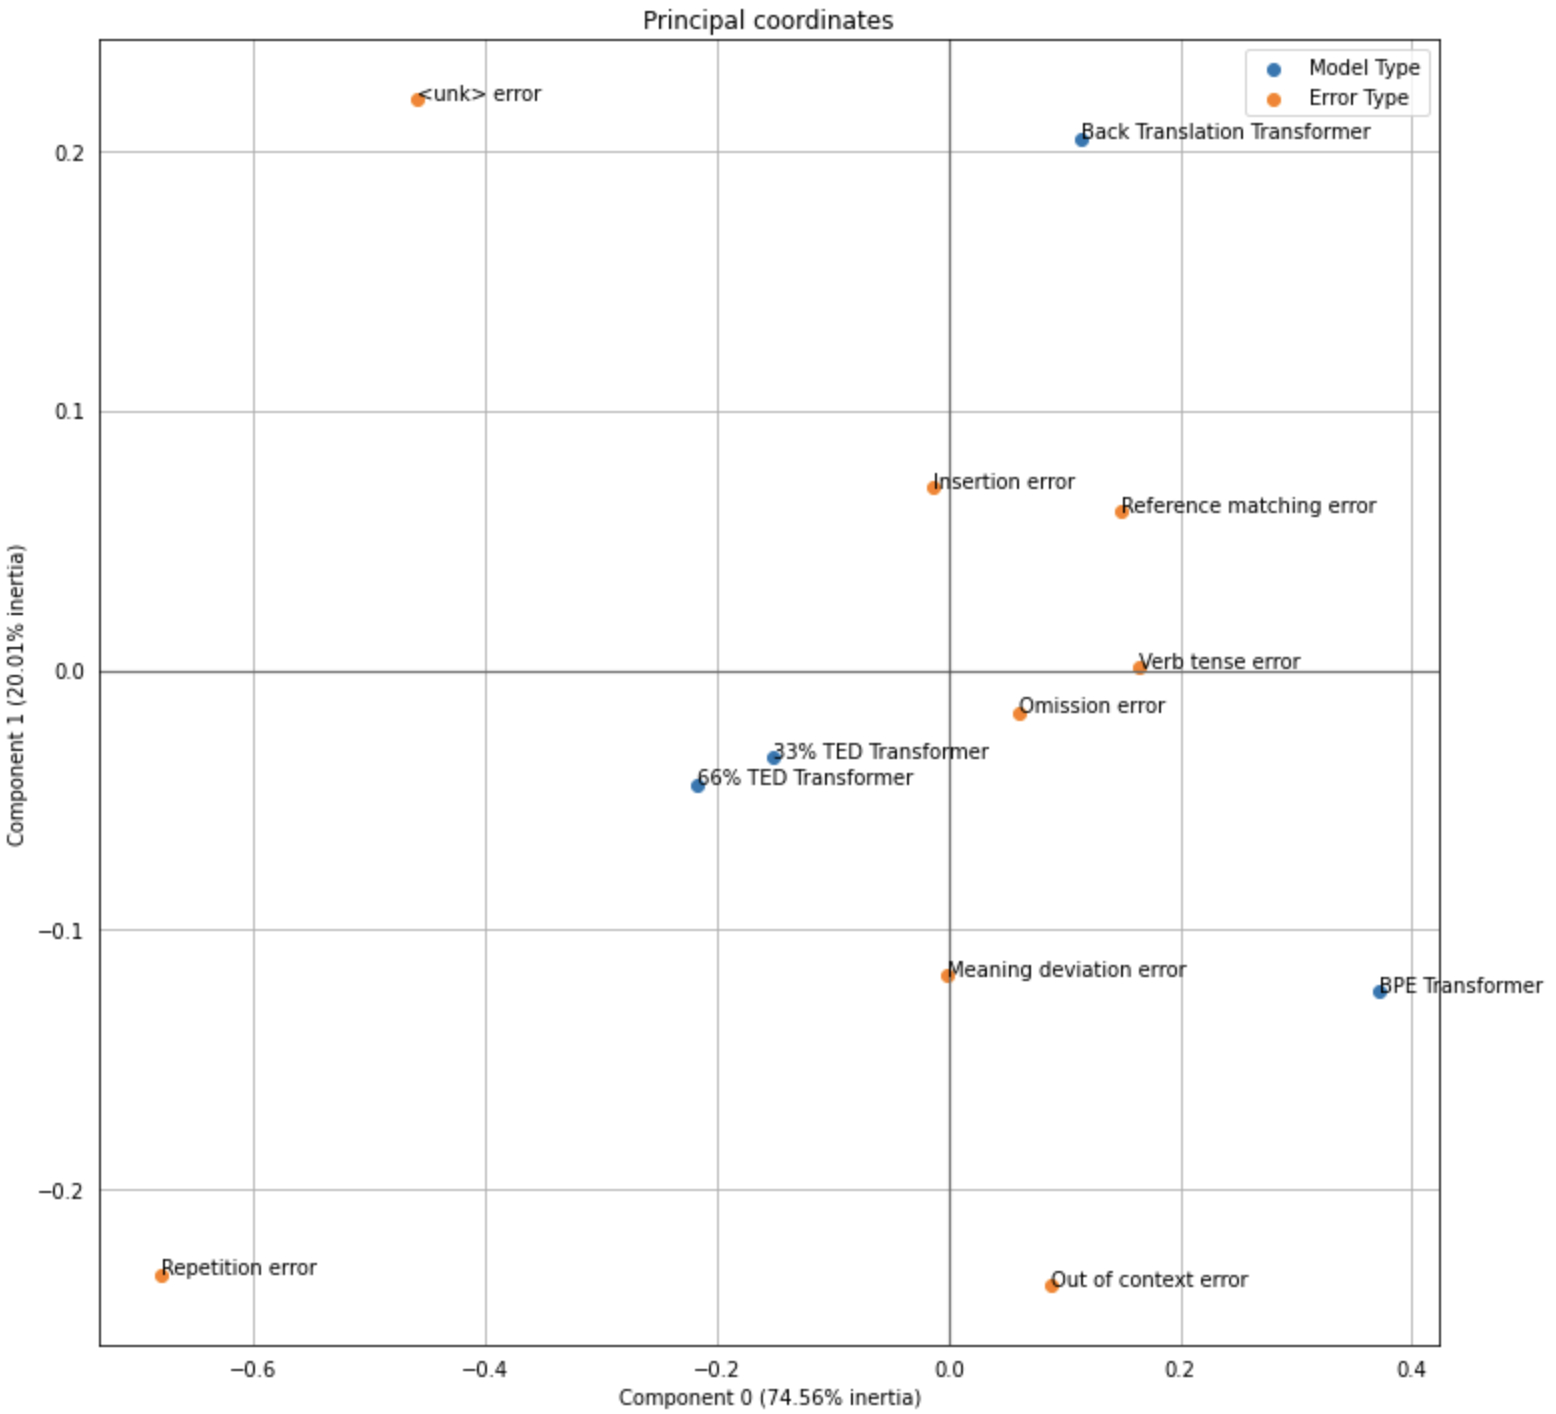
\includegraphics[keepaspectratio,scale=0.5]{chapter5_images/correspondence_model_error.png}
\caption{Correspondence analysis visualization comparing models and error classes}
\label{correspondence_model_error}
\end{figure*}

The algorithm has successfully fitted the dataset with an explained variance of 94.57\%, with about 74.56\% belonging to the first component and 20.01\% to the second component. This score indicates a very good representation of the data. Figure \ref{correspondence_model_error} shows the resulting visualization from the experiment. 

Some errors have stood out from the rest by denoting singular characteristics: Repetition, $<$unk$>$ and Out of context are all far from the origin, while the others are more concentrated in a smaller area. Reference Matching is located very close to Insertion, while Verb Tense is also close to Omission, indicating that error patterns of these pairs share similarities over the models. All these errors are located in an area with approximately the size of a quadrant, which means that despite the pairwise similarity is higher, similarity within the group also exists. 

Regarding models, the Back Translation model stands out from the others, while 33\% and 66\% are close, indicating that their error patterns share similarities. BPE seems to be isolated, so it has a weak relationship with the rest, but not as far from the origin as Back Translation. BPE error patterns are probably uncorrelated with Back Translation as they are the most distant models in the cartesian plane.

Below the findings of the experiment that relate both models and errors are listed, following a model-centered approach:

\begin{enumerate}
    \item BPE shows a positive correlation with the Omission error, being the model with the strongest relationship with this error. There is also some positive correlation with Verb Tense, Out of Context and Meaning Deviation. It is negatively correlated with the Insertion error and also with the $<$unk$>$ error, as its placed in about 180 degrees of them (which makes sense even more for $<$unk$>$ since the algorithm does not produce that error at all). At the same time it appears to have no correlation with the Repetition and Reference Matching errors, as it creates an angle near 90 degrees with them in the origin
    \item Both reduced models 33\% and 66\% possess similar relationships with errors. They are highly correlated with the Repetition error, still positively correlated with Meaning Deviation and $<$unk$>$ errors and negatively correlated with the Reference Matching and Verb Tense errors. They also seem to have almost no correlation with the Omission, Insertion and Out of Context errors
    \item Finally, the Back Translation model has high positive correlation with the Reference Matching and Insertion errors, and also some positive correlation with $<$unk$>$, while having almost no correlation with Verb Tense and Omission errors. It also has a strong negative correlation with the Repetition and Meaning Deviation errors, and in a smaller degree with Out of Context
\end{enumerate}

Some interesting hypothesis can be outlined based on the graphical inspection. Augmenting with data from a different domain induces the model to create translations that don't match the reference, potentially indicating that it finds synonyms for words of the same sentence. BPE seems to frequently omit words although it is also efficient against the Insertion of unnecessary words. Regarding the models trained on reduced TED, they seem to repeat the same words when they do not possess vocabulary knowledge to finish a sentence with certainty. Also, the reduced vocabulary seems to prevent the occurrence of synonyms, probably because of the limited options of words.

\subsubsection{Sentence complexity and error classes}

In this second round of Correspondence Analysis experiments, the dataset containing the binary flags indicating error classes per sentence has been grouped by complexity label and summed over the binary columns, generating another 2-way contingency table where the rows are CEFR complexity levels and columns represent the error classes. The explained variance indicates another successful representation of data: for both components it reaches 96.29\%, with a contribution of 64.28\% from the first component and 32.01\% from the second component. The resulting visualization can be seen in Figure \ref{correspondence_complexity_error}.

\begin{figure*}[tb]
\centering 
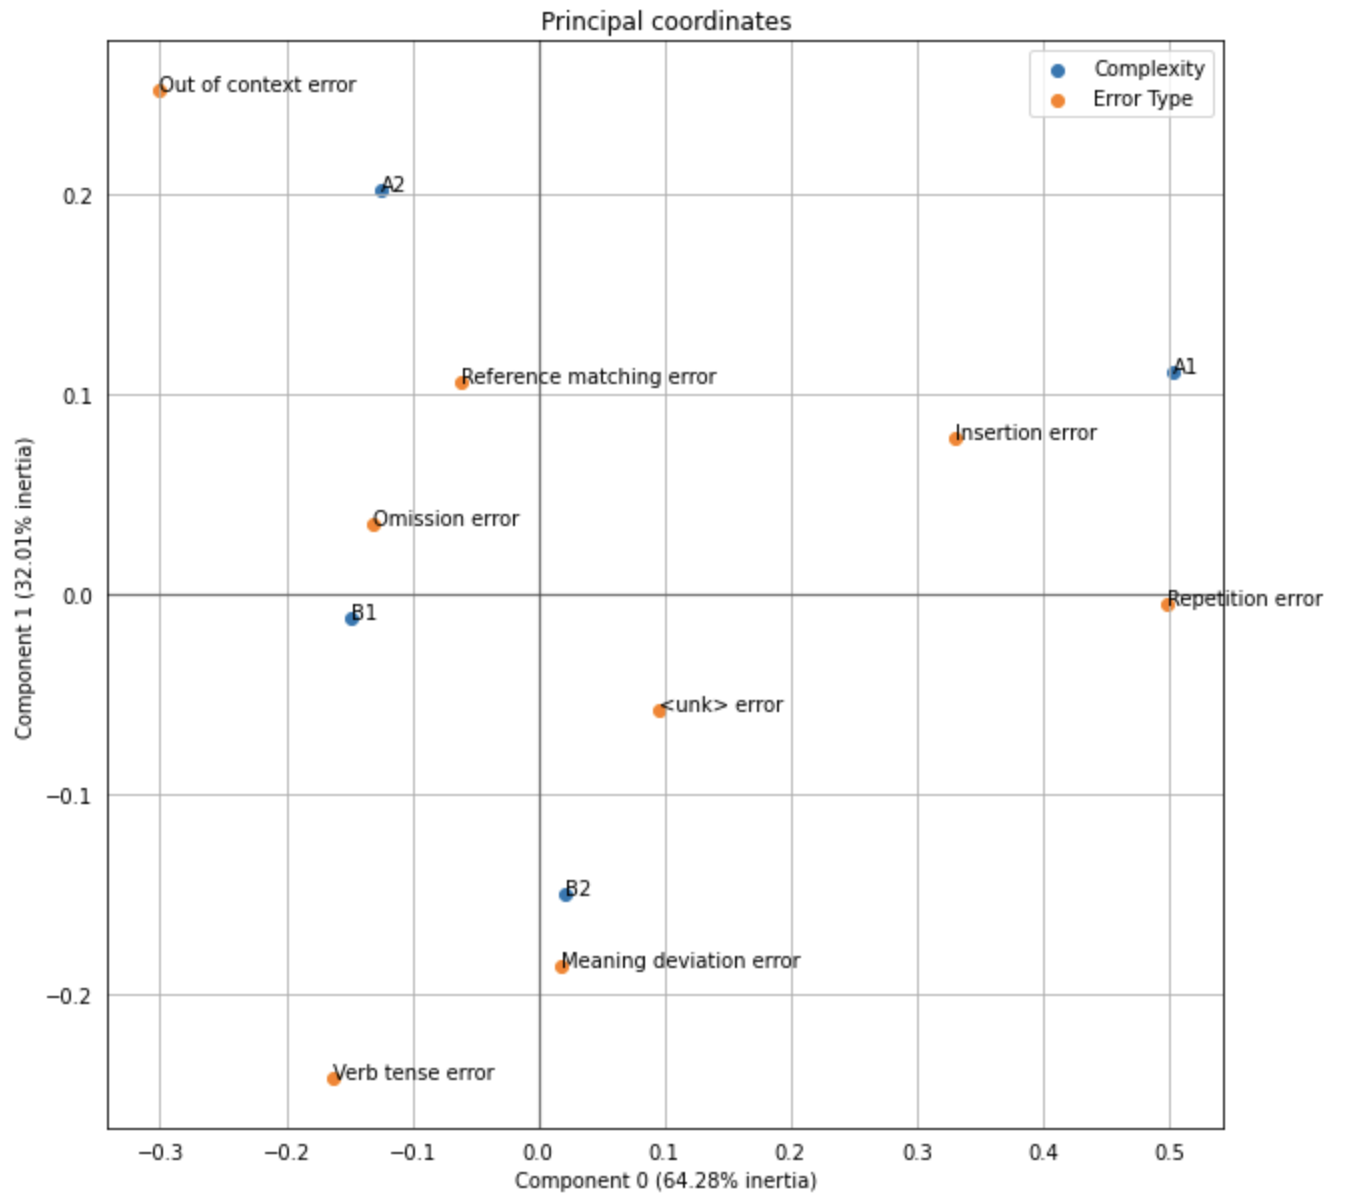
\includegraphics[keepaspectratio,scale=0.6]{chapter5_images/correspondence_complexity_error.png}
\caption{Correspondence analysis visualization comparing complexities and error classes}
\label{correspondence_complexity_error}
\end{figure*}

The categories that are most isolated and distinguish themselves from the others are the Repetition, Out of Context and Verb Tense errors as well as A1 complexity. The complexity labels are well distributed along the graph area, which indicate that they are probably segmenting well the sentences provided. The pairs B1 and B2, A2 and B1 are closer to each other, which makes sense as they represent consecutive complexities. The space between the error classes has also improved when compared to the last experiment, which means that they hold more unique patterns when talking of the relativities between their dimension and sentence complexity. The proximity of Insertion with Repetition indicates some similarity between these errors, which has also manifested in the previous experiment. Omission and Reference Matching errors are also close to each other, but this relation has only appeared in this experiment.

Regarding the category associations along both dimensions, all the positive, negative and absence of correlations derived from graphical inspection that were observed will be explained below. Although the graphical interpretation can be associated with correlation, it doesn't follow the pearson correlation formula for instance, it just considers associations between both dimensions derived from their co-occurrence matrix properties. We highlight the following observations:

\begin{enumerate}
    \item A1 shows potential for positive correlation with the Insertion, $<$unk$>$ and Repetition errors, negative correlation with Verb Tense and Omission errors and potential absence of correlation with the Reference Matching, Out of Context and Meaning Deviation errors
    \item The Figure indicates that A2 can be positively correlated with Reference Matching, Out of Context and Omission errors, probably negatively correlated with $<$unk$>$, Meaning Deviation and Verb Tense errors and lacks correlation with the Insertion and Repetition errors
    \item B1 has positive correlation with Omission, Verb Tense and Out of Context errors. Negative correlation shows up with Insertion, Repetition and $<$unk$>$ errors, and also apparently there is no correlation with the Reference Matching and Meaning Deviation errors
    \item Lastly, B2 seems to have positive correlation with Verb Tense, Meaning deviation and $<$unk$>$ errors, negative correlation with Out of Context and Reference Matching errors and absent correlation with the Repetition, Omission and Insertion errors
\end{enumerate}

The relations extracted through graphical interpretation have shown some interesting trends. The high explained variance and well distributed data points for both dimensions show that the algorithm's bias probably had a strong match with the data distribution bias, indicating that the categories have segmented very well the sentences. Qualitatively "simpler" errors such as Insertion and Repetition are usually correlated with lower complexities such as A1 and uncorrelated or negatively correlated with higher complexities, such as B1. Conversely, $<$unk$>$ and Meaning Deviation errors that are more associated with complex translations are usually positively associated with higher complexities such as B2 and negatively associated with lower complexities, such as A1. As the complexity points are scattered across the cartesian plane, the other errors create different relations with the complexity levels, but we believe they are situated in some sort of "medium level" complexity. It is a hard claim to make, it cannot be confirmed without an increased sample size, but it's one intuition that the results are providing.

\subsection{Consolidated result of the qualitative study}

Each experiment performed in the qualitative domain has presented a number of conclusions and hypothesis, but being able to visualize the whole picture based on the statements of the isolated experiments is a hard task. In this section we have filtered the most relevant patterns and findings and will try to establish a connection between them, aiming to provide a clear and concise view about the outcome of the qualitative analysis. 

The clarification of the qualitative results starts with a brief discussion about the expectations set for each experiment and a comparison of their results. Just comparing the average occurrence of errors between models cannot prove that one model indeed is more susceptible to that specific error than the other. Solely interpreting this average and comparing across dimensions (in our case, model-error or complexity-error) results in an analysis subjected to statistical flaws. This argument led the study to use the Fisher Exact hypothesis test, which has mathematical background to corroborate and complement the differences in averages and reveal potential disparities, given that the null hypothesis is rejected. On a second perspective, the Hierarchical Clustering algorithm segments the dataset and aggregates similar sentences into groups of clusters, each of them tracing an unique profile of error statistics that carry some weight when defining the error patterns of each technique, for instance. Although the interpretation is very subjective, it helps to reveal bidimensional associations between the model, error and complexity dimensions. Finally, the Correspondence Analysis experiment provides an easier interpretation along with richer and clearer associations between the dimensions of interest. All the categories belonging to the dimensions can be compared with clearly stated rules that can help to identify presence of positive or negative correlation, or even the absence of it. 

\begin{table}[t!]
  \caption{Main model-error conclusions extracted from qualitative experiments}
  \fontsize{10}{12}\fontfamily{phv}\selectfont
  \label{qualitative_error_model_consolidated}
  \centering
  {\footnotesize
  \begin{tabular}{| p{1.5cm} | P{1.1cm} | P{2.2cm} | P{2.5cm} | P{2.7cm} | P{2.3cm} |}
    \hline
    Relation-ship & Experiment & Back Translation & 33\% TED & 66\% TED & BPE Transformer \\
    \hline
    \multirow{3}{1.0cm}{Positive error correlation} & Fisher Exact Test & N/A & Meaning Deviation (vs BT), Repetition (vs BT, BPE), $<$unk$>$ (vs BT, BPE) & Meaning Deviation (vs BT), Repetition (vs BT, BPE), $<$unk$>$ (vs BT, BPE) & N/A \\
    \cline{2-6}
    & HC & Omission (cl1), $<$unk$>$ (cl1), Reference Matching (cl2) & Verb Tense (cl0, cl3), Reference Matching (cl0), Meaning Deviation (cl1), Omission (cl1, cl3), Out of Context (cl3) & Verb Tense (cl0), Reference Matching (cl2), Meaning Deviation (cl3), Out of Context (cl3) & Reference Matching (cl0, cl1, cl2), Verb Tense (cl0, cl1), Insertion (cl1), Meaning Deviation (cl1) \\
    \cline{2-6}
    & CA & Reference Matching, Insertion, $<$unk$>$ & Repetition, Meaning Deviation, $<$unk$>$ & Repetition, Meaning Deviation, $<$unk$>$ & Omission, Meaning Deviation, Out of Context, Verb Tense \\
    \hline
    \multirow{3}{1.0cm}{Negative error correlation} & Fisher Exact Test & Meaning Deviation (vs 33\%), Repetition (vs 33\%, 66\%), $<$unk$>$ (vs 33\%, 66\%) & N/A & N/A & Repetition (vs 33\%, 66\%), $<$unk$>$ (vs all) \\
    \cline{2-6}
    & HC & Out of Context (cl1), Meaning Deviation (cl1, cl3) & Reference Matching (cl1, cl2), Verb Tense (cl1) & Insertion (cl1), Verb Tense (cl1), Meaning Deviation (cl1), $<$unk$>$ (cl1), Reference Matching (cl1) & $<$unk$>$ (all), Omission (cl1) \\
    \cline{2-6}
    & CA & Repetition, Meaning Deviation, Out of Context & Reference Matching, Verb Tense & Reference Matching, Verb Tense & Insertion, $<$unk$>$ \\
    \hline
    \multirow{3}{1.0cm}{Almost zero correlation} & Fisher Exact Test & Omission, Out of Context, Reference Matching, Insertion, Verb Tense & Omission, Out of Context, Reference Matching, Insertion, Verb Tense & Omission, Out of Context, Reference Matching, Insertion, Verb Tense & Omission, Out of Context, Reference Matching, Insertion, Verb Tense \\
    \cline{2-6}
    & HC & Verb Tense (cl0, cl1, cl3) & Out of context (cl3) & Out of context (cl3) & Out of context (cl3) \\
    \cline{2-6}
    & CA & Verb Tense, Omission & Omission, Out of Context, Insertion & Omission, Out of Context, Insertion & Repetition, Reference Matching \\
    \hline
\end{tabular}}
\end{table}

\subsubsection{Models and error classes}

The main goal of the study is to be able to track error patterns and also correlate them to a specific technique, but as this may represent only a subset of the problem, other relevant dimensions were added aiming to refine its explication. Sentence complexity has been chosen as an auxiliary dimension for this, others could be considered, but unfortunately resources are scarce to increase the depth, specially considering low-resource constraints. Therefore, the explored domain is limited to these 3 dimensions. The principal results of the associations that belong to the core goal (correlate models and error patterns) are displayed in Table \ref{qualitative_error_model_consolidated}, they are split among positive, negative and absence of correlation, considering the incidence of error classes and their relationship with each model.

Notice that each error class relationship outlined in a cell has in parenthesis the scenario where it was revealed. In the Fisher experiment, the classes reported always consider a comparison against another model, whereas in HC each conclusion was extracted from a specific cluster, and in CA the process is easier since it is inspected graphically, it doesn't need a reference. The correlation categories with no findings were filled with "N/A". The almost zero correlation row had a different motivation for each experiment: in Fisher it basically complements the classes that didn't reject the null hypothesis of positive and negative correlation, while HC if the share of sentences per class between clusters varies but the error average remains, it falls into this category. Finally, in CA there is no inference to be made, since the interpretation guidelines already provide a clear diagnostic.

When reading the results, it is important to keep in mind that there is quantitative evidence available to reinforce the argument that results of the CA algorithm are more reliable than the ones from HC. This is due to the explained variance achieved of about 95\%, which is considered to be optimal, while a silhouette coefficient of 0.2320 is notably far from the desired target of 1. This corroborates the assumptions made when writing the interpretations in the following paragraphs, which will follow the logic that the findings of CA will be considered stronger statistically speaking than the ones from HC.

The Back Translation Transformer is probably more subjected to the Reference Matching error based on results from HC and CA, with potentially some synergies with the Insertion error denoted by CA. The hypothesis of the Omission and $<$unk$>$ errors being positively correlated are discarded by (1), the suggestion from CA that the former has almost zero correlation and (2), the Fisher Test accusing that the latter is less frequent in this model versus the reduced TED models, which seems to be stronger since the angle shown in CA is bigger than 60 degrees. The BT model also spawns less often the Out of Context error according to CA, which is also true for Repetition and Meaning Deviation, backed by CA and Fisher (at least when compared to low-resource models). Lastly, the Verb Tense error seems to be supported in unanimity that it isn't correlated with BT at all, and a similar trend is followed by Omission, which is supported by Fisher and CA.

As already noticed before, both the 33\% and 66\% TED models share similar results in all experiments. The Fisher test and CA indicate that the Repetition and Meaning Deviation errors are common errors produced by these models. They also produce the $<$unk$>$ token a lot more when compared to BT and BPE based on Fisher, but its hard to ensure this since CA tells a different story in the absence of correlation part. Speaking of correlation absence, both CA and Fisher test tell that the incidence of the Omission, Insertion and Verb Tense errors is indifferent with an increase or decrease of sentences evaluated by the 33\% and 66\% TED models. This may also apply to the Out of Context error, according to HC and Fisher, but that affirmation is made without agreement by CA (given the negative correlation hypothesis). Regarding negative correlation, it seems that the Reference Matching and Out of Context errors are pointed out to occur less with the models trained on reduced TED by HC and CA.

Finally, considering the BPE Transformer, the CA row in Table \ref{qualitative_error_model_consolidated} shows that the occurrence of Meaning Deviation, Verb Tense, Out of Context and Omission errors is directly proportional to an increase in the number of sentences generated by such model. The $<$unk$>$ token has a negative correlation with the model, meaning that it is efficient against it, according to all models. In the meanwhile, CA indicates that Insertion also should also not spawn a lot when using BPE and Fisher tells the same regarding Repetition. Regarding absence of correlation, CA points that the Reference Matching error is uncorrelated with the model.

These were the straightforward findings to correlate models and errors, however there are some reflections and conclusions that come as a side product but are not evident in those statements. For instance, one of such statements is that augmenting with data from a different domain induces the model to create translations that don’t match the reference. This cannot be interpreted as a rule, further studies are required to establish this pattern, but developing this hypothesis wouldn't be even possible without applying the aforementioned algorithms. Other similar statements include the fact that BPE seems to frequently omit words although it is also efficient against the Insertion of unnecessary words.

Models under heavier low-resource constraints such as the ones trained on the reduced TED seem to repeat the same words when they do not possess vocabulary knowledge to finish a sentence with certainty (according to CA and Fisher). Also, the reduced vocabulary seems to prevent the occurrence of synonyms, probably because of the limited options of words. In all experiments, both the models trained on 33\% and 66\% of the dataset share similar error distributions, are situated nearby in graphical visualizations (CA) or segmented in clusters with a similar share of sentences. This may represent a proof that the experiments shows some correlation between their error patterns.

\subsubsection{Sentence complexity and error classes}

A similar thought process was conducted for the experiments that aimed to correlate sentence complexity and error classes. As complexity was included more as a complement to understand the error patterns of models, it doesn't make sense to analyse each complexity level in the same manner as done for each model that participated in the study, as done in the previous section. Also, there is no clear value for instance in correlating the models directly with complexities. The objective here is to understand how complexity impacts the error patterns, if the criteria established for the CEFR segmentation performed made sense and how it is reflected on the distribution of errors. A proxy used to validate this is checking if an increase in complexity level leads to an increase, decrease or no difference in the amount of errors made.

\begin{table}[h!]
  \caption{Main complexity-error conclusions extracted from qualitative experiments}
  \fontsize{10}{12}\fontfamily{phv}\selectfont
  \label{qualitative_complexity_model_consolidated}
  \centering
  {\footnotesize
  \begin{tabular}{| p{3.0cm} | P{2.0cm} | P{8.2cm} |}
    \hline
    Relationship & Experiment & Errors that are proportional to complexity \\
    \hline
    \multirow{3}{3.0cm}{Errors directly proportional with complexity} & Fisher Exact Test & Reference Matching, Omission (except for A2|B2), Out of Context (except for A2|B2), Verb Tense, Meaning Deviation \\
    \cline{2-3}
    & HC & Reference Matching (cl0), Verb Tense (cl1, cl3), Meaning Deviation (cl1), Omission (cl1, cl3) \\
    \cline{2-3}
    & CA & Insertion (A1), Repetition (A1), $<$unk$>$ (A1, B2), Meaning Deviation (B2), Verb Tense (B1, B2), Reference Matching (A2), Out of Context (A2, B1), Omission (A2, B1) \\
    \hline
    \multirow{3}{3.0cm}{Errors inversely proportional with complexity} & Fisher Exact Test & Insertion (except for A1|B2, A2|B2), $<$unk$>$ (except for A1|B2, A2|B2) \\
    \cline{2-3}
    & HC & $<$unk$>$ (cl1), Insertion (cl1), Meaning Deviation (cl3) \\
    \cline{2-3}
    & CA & Omission (A1), Reference Matching (A2, B2), Out of Context (A2, B2), Insertion (B1), Repetition (B1), $<$unk$>$ (A2, B1), Meaning Deviation (A2), Verb Tense (A1) \\
    \hline
    \multirow{3}{3.0cm}{Almost zero correlation with complexity} & Fisher Exact Test & Repetition \\
    \cline{2-3}
    & HC & Out of context (cl3), Verb Tense (cl0) \\
    \cline{2-3}
    & CA & Insertion (A2, B2), Repetition (A2, B2), Meaning Deviation (A1, B1), Out of Context (A1), Meaning Deviation (A1), Reference Matching (B1), Omission (B2) \\
    \hline
\end{tabular}}
\end{table}

With the motivations explained, Table \ref{qualitative_complexity_model_consolidated} contains the results. Notice that each technique share a similar reference of comparison as before, which is represented between parenthesis. HC highlights cluster averages, Fisher compares which tests did not show a difference for higher versus lower complexities and CA tells the type of correlation between errors and complexities, similarly to what happened for the model-error pair. The same analogy that CA had a better performance when fitting the dataset, and hence will weight more on the final outcome than other techniques can be applied here.

Most of the error classes (5 out of 8) stood out from the rest for being directly proportional with complexity: Reference Matching, Omission, Out of Context, Verb Tense and Meaning Deviation. Some of them in unanimity, others supported by strong evidence provided by some experiments but not from all. In addition, there are some errors that appear to have an inverse relationship with complexity: Insertion and $<$unk$>$, backed by all the experiments. By elimination, all the experiments but HC have indicated that the Repetition error seem to not be affected by complexity, so presenting more complex or less complex sentences to a model is unlikely to change its probability to happen. It is the only error that is potentially more prone to be modified with the change of a model or a technique rather than the complexity of the sentence.

There is a story to tell based on the results that go beyond the straightforward interpretation of them: all experiments indicate that the categories have segmented very well the sentences. The position of the complexity categories in the CA plot in Figure \ref{correspondence_complexity_error} are a strong evidence, along with the hypothesis test not finding any relevant changes between any pairs. To some extent, but in a less evident manner, the distribution of errors per cluster also supports the argument that a good segmentation took place. The algorithm has agglomerated sentences with similar complexity in clusters 3 and 4, despite the fact that it didn’t receive this information beforehand.  Its interesting to note that errors have found more occurrences in specific complexity levels. Not always they were directly proportional, but in most times (62.5\% to be precise) errors had a trend to increase based on an increase in the complexity of sentences presented to a model, while 25\% were inversely proportional and 12.5\% showed no difference. A worrisome scenario would happen if most errors showed no correlation with the complexity categories, but numbers show that this is far from reality.


% \begin{table}[h]
%   \caption{Qualitative results interpretation for the unsupervised model-error analysis}
%   \fontsize{10}{12}\fontfamily{phv}\selectfont
%   \label{tab:table4-multidim-results}
%   \centering
%   {\footnotesize
%   \begin{tabular}{| p{0.80cm} | P{0.80cm} | P{1.35cm} | P{1.2cm} | P{1.6cm} | P{1.35cm} | P{1.2cm} | P{1.4cm} | P{1.6cm} |}
%     \hline
%     \multirow{2}{0.8cm}{1st Model} & \multirow{2}{0.8cm}{2nd Model} & \multicolumn{3}{|P{4.1cm}|}{Hierarchical Clustering} & \multicolumn{3}{|P{4.0cm}|}{Correspondence Analysis} & \multirow{2}{1.6cm}{Discussion} \\
%     \cline{3-8}
%     & & Common Errors & Rare Errors & Result & Common Errors & Rare Errors & Result & \\
%     \hline
%     33\% Reduced TED Model & 66\% Reduced TED Model & Insertion and $unk$ & Repetition and Verb Tense & They share similar proportions in the clusters they appear in & Repetition and $unk$ & Similar word choice and Verb tense & The dots that represent both models are very close & Both indicate that they have very similar error patterns and stand out from the others\\
%     \hline
%     \multicolumn{2}{|P{1.9cm}|}{BPE} & Out of Context, Sentence Choice, Omission and Verb Tense & $unk$ and Repetition & Verb Tense stands out as common, Repetition and $unk$ as uncommon & Omission, Out of Context, Sentence Choice and Verb Tense & $unk$ and Insertion & Model positions itself far from the others and with different correlations & Common errors converge completely and $unk$ is unrelated in both \\
%     \hline
%     \multicolumn{2}{|P{1.9cm}|}{Back Translation} & Similar Word Choice, Omission and Sentence Choice & Repetition, $unk$ and Out of Context & $unk$ and Repetition perform bad while Similar Word choice stands out in all clusters & Similar Word Choice and Insertion & Out of Context, Sentence Choice and Repetition & Model positions itself far from the others and with different correlations & Similar word choice stands out while Repetiton and Out of Context are unrelated \\
%     \hline
% \end{tabular}}
% \end{table}

% \begin{table}[h]
% \caption{Transfer learning and subword embeddings translation results}
% \fontsize{10}{12}\fontfamily{phv}\selectfont
% \begin{tabular}{| p{2.5cm} | p{1.5cm}  | p{1.0cm}  | p{0.9cm}  | p{1.1cm}  | p{1.5cm}  | p{1.0cm}  | p{0.9cm}  | p{1.1cm} |}
%     \hline
%     \multirow{2}{2.5cm}{Technique applied} & \multicolumn{4}{|p{5.0cm}|}{Tatoeba} & \multicolumn{4}{|p{5.0cm}|}{TED}\\
%     \cline{2-9}
%     & Sacrebleu & NLTK BLEU & Batch Size & Epochs & Sacrebleu & NLTK BLEU & Batch Size & Epochs \\
%     \hline
%     None & 57.99 & 74.07 & 512 & 54 & 25.24 & 65.36 & 34 & 29\\
%     \hline
%     \mbox{Fast Text} & 56.96 & 69.91 & 512 & 50 & 24.07 & 61.69 & 30 & 45\\
%     \hline
%     \mbox{Fast Text} (encoder + decoder Gigaword) & N/A & N/A & N/A & N/A & 24.54 & 61.76 & 32 & 89\\
%     \hline
%     \mbox{Fast Text} (source recommendations) non-binary loading (encoder + decoder Gigaword) & N/A & N/A & N/A & N/A & 21.26 & 52.31 & 32 & 80\\
%     \hline
%     Subword BPE & \textbf{66.63} & \textbf{83.02} & 512 & 40 & \textbf{40.26} & \textbf{72.20} & 32 & 40\\
%     \hline
% \end{tabular}
% \end{table}
 
\chapter{Conclusion}

Over the course of the previous chapters a lot of context was given, the main problem to be addressed was defined, and after reviewing the literature some techniques were elected to be analysed. The analysis of the results was customized to increase its depth. The goal was to be able to interpret the technique's translation error patterns despite the challenge of pursuing this qualitative path, which is usually overlooked in the NMT field.

We have started this work providing context of how the NLP field evolved to tackle Machine Translation and the challenges that arised from it. The scarcity of Portuguese papers about NMT at the time of writing provided additional technical and language intrinsic challenges to contribute to the field, meanwhile it was also seen as an inspiration to make more impact. All Portuguese language challenges were categorized in the main aspects that linguistics state for all languages in Chapter \ref{machine_traslation_challenges}. The language was rated to some subjective level of difficulty in each of those criteria to provide context of the work's complexity. Subsequently, the traditional ways of representing and modelling natural language were presented, along with how they evolved to contemplate the task of Machine Translation. Popular NLP algorithms such as word2vec were presented and explained in equations to provide intuition of the common ways Artificial Intelligence has to tackle NLP related tasks.

After providing context on some fundamentals of NLP, we presented the recurrent neuron in a simplified graph and analysed how it fits into one of the first NMT algorithms to become widespread \cite{cho-etal-2014-learning}. The main strengths and drawbacks of the algorithm were presented, some of them already addressed by the same authors, that some months later came up with a variant that addressed the fixed length vector issue \citet{bahdanau2016neural}. These models represent the pioneer studies in this area, they have also inspired studies using other neural architectures. Yet one architecture has prevailed upon the others for some time: the Transformer. The Transformer was introduced later, trying to provide implementation details that were complex to grasp when reading the original paper. Not only the architecture was shown in detail, but all the other components that help the Transformer reach its performance, such as beam search, positional encoding and the attention mechanism. Later, some Transformer variants that became popular in the literature were commented, exploring not only architecture variations but also the training objective.

In Chapter \ref{low_res_context} the definition of the low-resource term is given, along with the motivation that led us to follow this trend. Some practical challenges for performing the experiments were also discussed, mentioning how we approached the problem or how issues were addressed whenever possible. Subsequently, all the theory behind NMT related techniques such as Subword Embeddings, Transfer Learning (for word embeddings) and Back Translation was presented. Some of those techniques weren't created specifically for tackling low-resource issues, BPE for instance was aiming at more efficient embeddings that could solve the $<$unk$>$ token issue. Back Translation is one example of technique aligned with Data Augmentation purposes of solving low data availability by expanding the dataset without the need of extra datasets. 

Lastly, in chapter 5 the hypothesis we would like to clarify experimentally are mentioned, the connection between them and the experiment design is established, along with the expectations that were set for each one of them. The chapter starts by describing the datasets and the experimentation environment. Important information for reproducibility is given here, along with the assessment metrics. Later, the quantitative study was presented, where we compare different dataset content restrictions in experiment 1, and discover that low data availability has a less harmful effect than expected, with an increase from 83.3\% to 100\% of the dataset size even hindering performance. In experiment 2, the utility of subword embeddings and transfer learning is confronted, resulting in a worse performance than expected for Fast Text and a promising achievement for BPE. The effectiveness of Back Translation to address low resource is tested in experiment 3, where we discover that same domain augmentation overcomes different domain and that a synthetic ratio of 16.6\% yield the best results. Finally, we compare our best models against the Google Translate benchmark in experiment 4, and discover that we are able to reach 77.1\% of its performance, using the most complete assessment metric (sacrebleu). 

The qualitative study started by mentioning important challenges that to some extent had an impact on the outcome of the analysis, such as data quality issues and interaction bias with the translator. We don't believe they are relevant enough to invalidate any of the conclusions. Subsequently, the qualitative criteria was presented, which is basically composed of 2 dimensions: the error classes and the sentence complexities (based on CEFR \cite{COE}). The qualitative experiments are presented in the sequence, all focused on understanding bidimensional correlation between error classes and complexity or model plus technique. In such experiments, we use Fisher Exact Test to extract statistically relevant differences in both dimension pairs, Hierarchical Clustering to segment the dataset and identify similar error patterns within the clusters and Correspondence Analysis to find visual correlations between the dimension pairs. 

Our findings show that some techniques are more vulnerable to some error classes and efficient against others. In some cases all algorithms identify the same relationship between 2 dimensions, providing stronger evidence that the choice of a technique indeed has an impact on the patterns of errors performed. For instance, all the algorithms show that Back Translation is efficient against the Meaning Deviation error and uncorrelated with Verb Tense, while the models trained on a reduced dataset are more vulnerable to the Meaning Deviation and Repetition errors. All experiments interpret both reduced models as having a similar relationship with the error classes, indicating that their error patterns probably converge. According to CA, BPE seems to be vulnerable to the Meaning Deviation, Verb Tense, Out of Context and Omission errors while still efficient against Insertion and, obviously, the $<$unk$>$ error.

Regarding complexity and error classes, the analysis has focused on understanding what relationship error classes have with an increase in complexity. The goal is to validate if the incidence of errors is higher or smaller when complexity increases, to check if that class is prone to a change purely based on complexity of if it is more correlated with the model or technique error patterns. The experiments show that most of the error classes (5 out of 8) behaved as directly proportional with complexity: Reference Matching, Omission, Out of Context, Verb Tense and Meaning Deviation. Meanwhile there are other errors that appear to have an inverse relationship with complexity, Insertion and $<$unk$>$, supported by all the experiments. One error possess no correlation with changes in complexity, so presenting more complex or less complex sentences to a model is unlikely to change its probability to happen, which is the repetition error. It is the only error that is potentially more prone to happening with a model or a technique rather than with a different complexity.

The reader is encouraged to go through the chapters to better understand the findings mentioned here. The gaps we couldn't fill in our analysis and interesting directions to be explored will be mentioned in the next section.

\section{Next steps}

There are mainly 2 directions of improvement for this study: focusing on going further in depth in the qualitative analysis, by adding more sentences, qualitative criteria or experiments, or expanding its scope to contemplate more techniques. Both directions can be valuable to be explored, depending on the use case and objective. Reproducing the same sequence of experiments shown here can be promising specially for other researchers that wish to understand how can they address specific translation errors in their models. 

Unfortunately, our sample size of unique sentences could not go much further than 100 sentences, as the interaction with the translator required a budget that was limited. Because of this, we acknowledge the potential of enhancing the criteria if a bigger sample is analysed by a group of translation experts. Maybe there are other types of errors that could be covered, or even a category that was set but could be split into more granular categories to add more details. The qualitative criteria would benefit from receiving more samples and the review of other linguistic experts, thriving diversity and becoming more robust. That would help solving in more depth the subjectivity challenge and bringing more representativeness for the analysis. 

Considering the algorithms used to extract bimensional associations, there might be also other algorithms that can be applied to tackle the same problem and reach a good fit when applied to the datasets used. This would enable the study to also derive other conclusions that haven't been considered here and could be useful. Hierarchical Clustering, Correspondence Analysis and Fisher Exact Test seem to complement each other very well, but the possibility of another algorithm to reveal unknown correlations is real.

Expanding the scope to analyse qualitatively more recent NMT algorithms can also help to understand if they are being efficient in addressing the known flaws of the vanilla Transformer, for instance. Maybe they are improving translation errors of some kind while sacrificing others, and perhaps a technique which a different qualitative profile can show up as a good complement for that model. This is a dimension of NMT performance that deserves further research and investigation, and has the potential to reveal new issues and unlock more consistent translation quality for modern Machine Translation models.

\backmatter
\bibliographystyle{coppe-unsrt}
\bibliography{example}

% \appendix
% \chapter{Algumas Demonstra{\c c}\~oes}

% Fazer uma releitura da dissertação como um todo, precisa ser breve e tocar nos pontos principais, não escrever mais do que duas páginas. 

% \definecolor{maroon}{cmyk}{0,0.87,0.68,0.32}
% \begin{table}[h]
% \caption{Next steps chronogram}
% \label{tab:citation}
% \centering
% {\footnotesize
% \begin{tabular}{| p{6cm} | p{3.5cm} | p{1.5cm} | p{3.5cm} |}
% \hline
% Deliverable & \verb|Start Date| & \verb|Duration| & \verb|End Date|\\
% \hline
% Run dataset experiments without subword, embeddings or data augmentation for CBIC paper & \verb|06/05/2021| & \verb|7 days| & \verb|13/05/2021|\\
% Run dataset experiments with subword and embeddings for CBIC paper & \verb|13/05/2021| & \verb|7 days| & \verb|20/05/2021|\\
% Implement data augmentation techniques & \verb|13/05/2021| & \verb|7 days| & \verb|20/05/2021|\\
% Run dataset experiments with data augmentation for CBIC paper & \verb|20/05/2021| & \verb|7 days| & \verb|27/05/2021|\\
% Review paper to CBIC (if possible to publish) & \verb|20/05/2021| & \verb|7 days| & \verb|27/05/2021|\\
% Submit paper to CBIC (if possible) & \verb|29/05/2021| & \verb|1 day| & \verb|30/05/2021|\\
% Properly fill equations and enrich discussion regarding dissertation & \verb|03/06/2021| & \verb|14 days| & \verb|17/06/2021|\\
% Come up with a formula to analyse whether a training setup will work on a single GPU based on parameters & \verb|17/06/2021| & \verb|21 days| & \verb|08/07/2021|\\
% \rowcolor{maroon!20} 
% Dissertation 1st review & \verb|24/06/2021| & \verb|7 days| & \verb|01/07/2021|\\
% Rethink the set of experiments to dissertation based on presented techniques & \verb|08/07/2021| & \verb|7 days| & \verb|15/07/2021|\\
% Run dissertation remaining experiments and fill results & \verb|08/07/2021| & \verb|21 days| & \verb|29/07/2021|\\
% Review, identify gaps and improve dissertation & \verb|15/07/2021| & \verb|14 days| & \verb|29/07/2021|\\
% \rowcolor{maroon!20} 
% Dissertation 2nd review & \verb|29/07/2021| & \verb|7 days| & \verb|05/08/2021|\\
% Write STIL paper & \verb|05/08/2021 (?) (TBD)| & \verb|14 days| & \verb|12/08/2021 (?) (TBD)|\\
% Run experiments to STIL & \verb|12/08/2021 (?) (TBD)| & \verb|7 days| & \verb|19/08/2021 (?) (TBD)|\\
% \rowcolor{maroon!20} 
% Examiner group proposition & \verb|12/08/2021| & \verb|7 days| & \verb|19/08/2021|\\
% STIL paper review & \verb|19/08/2021 (?) (TBD)| & \verb|7 days| & \verb|26/08/2021 (?) (TBD)|\\
% Act upon feedbacks given from examiner group & \verb|19/08/2021| & \verb|7 days| & \verb|26/08/2021|\\
% Submit paper to STIL & \verb|26/08/2021 (?) (TBD)| & \verb|1 day| & \verb|27/08/2021 (?) (TBD)|\\
% Review, identify gaps and improve dissertation & \verb|26/08/2021| & \verb|21 days| & \verb|16/09/2021|\\
% \rowcolor{maroon!20} 
% Dissertation final review & \verb|16/09/2021| & \verb|7 days| & \verb|23/09/2021|\\
% \rowcolor{maroon!20} 
% Dissertation presentation & \verb|23/09/2021| & \verb|7 days| & \verb|30/09/2021|\\
% \hline
% \end{tabular}}
% \end{table}

  
% \title{Tackling neural machine translation in low-resource settings: a Portuguese case study}

% % \author{Arthur T. Estrella\inst{1}, João B. O. Souza Filho\inst{2}}
% % \author{Author 1\inst{1}, Author 2\inst{2}}


% % \address{
% % % Instituto Alberto Luiz Coimbra de Pós-Graduação e Pesquisa de Engenharia -- Federal University of Rio de Janeiro (UFRJ)\\
% % Electrical Engineering Program (PEE/COPPE), Federal University of Rio de Janeiro\\ PO Box 68504, RJ 21941-972, Brazil
% % \email{atelles@coppe.ufrj.br, jbfilho@poli.ufrj.br}
% % % Department W, University X\\ Postal Code Y, City Z, Brazil
% % % \email{xxx@xxx.xxx.xx, xxx@xxx.xxx.xx}
% % }

% \begin{abstract}
% Neural machine translation (NMT) nowadays requires an increasing amount of data and computational power, so succeeding in this task with limited data and using a single GPU might be challenging. Strategies such as the use of pre-trained word embeddings, subword embeddings, and data augmentation solutions can potentially address some issues faced in low-resource experimental settings, but their impact on the quality of translations is unclear. This work evaluates some of these strategies on two low-resource experiments beyond just reporting BLEU:  errors are categorized on the Portuguese-English pair with the help of a translator, considering semantic and syntactic aspects. The BPE subword approach has shown to be the most effective solution, allowing a BLEU increase of 59\% p.p. compared to the standard Transformer.
% \end{abstract}

% % Neural machine translation (NMT) exploits deep models that require an increasing amount of data and computational power. However, succeeding in this task with limited data and using a single GPU can be challenging. Techniques such as pre-trained word embeddings, subword embeddings and data augmentation can potentially address some low-resource issues, but their impact on the quality of translations is unknown. This work evaluates the quantitative impact of such techniques and also classifies translation errors made by the model on the Portuguese-English pair, with a complexity drill down. This allows a better inference of the relations between translation quality aspects and the usual assessment metrics.
     
% % \begin{resumo} 
% % \end{resumo}

% \section{Introduction}

% % ------------- Joao
% % Since the creation of the Neural Machine Translation (NMT) branch, many solutions seem to have ignored the associated computational burden, solely focusing in surpassing the state-of-the-art. As a consequence, most models have been progressively adopting deeper architectures, increasing the number of parameters and requiring huger datasets. The excessive focus on boosting performance regardless complexity deviated researchers from a further criticism over how the proposed architectures address the translation task, if simpler models can achieve a similar performance than more complex ones, and how to cope with translation errors.

% Since the rise of the Neural Machine Translation (NMT) branch, many solutions solely focused on surpassing the state-of-the-art, ignoring the associated computational burden. Thus, most models have been progressively adopting deeper architectures, hugely increasing the number of network parameters and, as a result, the dependence on more extensive datasets. The excessive focus on boosting performance regardless of complexity deviated the researchers from a more profound criticism over how such architectures address the translation task, if more cost-effective models can be proposed, and how to better cope with translation errors.

% % Later, some efforts have been dedicated to the proposition of models and strategies to allow the NMT systems to achieve relevant performance, but considering less-complex and computing demanding solutions. 

% % ------------- Joao (VALE DESTACAR QUE PRE-TRAINED WORD EMBEDDINGS É A MESMA COISA QUE PRIOR DEFINITION. ACRESCENTEI BACK TRANSLATION QUE ESTAVA FALTANDO)
% % Low-resource domains in NMT can be roughly defined as practical development scenarios wherein the GPU memory and data available to train the models are more severely limited. Some techniques can potentially help under those circumstances, like the use of pre-trained word embeddings, the prior definition of the starting weights of the network embedding layer \cite{qi-etal-2018-pre} (warm-start), or even the production of embeddings at a subword level \cite{DBLP:journals/corr/SennrichHB15}. 

% Low-resource NMT domains are defined as practical development scenarios wherein the GPU memory and the amount of data available to train some model are limited. Some techniques can potentially help under those circumstances, as the prior initialization of neural network embedding weights \cite{qi-etal-2018-pre} with pre-trained word embeddings, the production of embeddings at a subword level \cite{DBLP:journals/corr/SennrichHB15} or data augmentation with a monolingual dataset \cite{DBLP:journals/corr/SennrichHB15a} (also known as back-translation). 

% % ------------- Joao (REDUZI ESSE PARAGRAFO TENTANDO MANTER A QUALIDADE)
% % To the best of our knowledge, experimental studies considering low-resource contexts, as discussing and evaluating the cost-effectiveness of strategies aiming to circumvent the practical issues faced in such domains, especially considering the Portuguese-to-English pair are missing in the literature. Many previous works only focus on optimizing metrics such as BLEU. Despite its usefulness, this index is limited due to only accounting for matches of fixed number of n-grams, penalizing correct but different lexical translations.

% To the best of our knowledge, experimental studies discussing and evaluating the cost-effectiveness of strategies aiming to circumvent the practical issues faced with low-resource domains, especially considering the English-to-Portuguese pair, are missing in the literature. Many previous works only focused on optimizing metrics such as BLEU. Despite its usefulness, this index is limited due to only accounting for matches of a fixed number of n-grams, penalizing correct but different lexical translations.

% % ------------- Joao (REDUZI ESSE PARAGRAFO TENTANDO MANTER A QUALIDADE)
% % This work uses Transformers \cite{DBLP:journals/corr/VaswaniSPUJGKP17} as one state-of-the-art reference model to  experimentally evaluate the impact of strategies like transfer learning, sub-word modeling, and data augmentation in the translation quality, considering a low-resource setting, characterized by the use of small and medium size databases, only one average size GPU, and the English-to-Portuguese pair. Additionally, a qualitative analysis over the translation errors produced by the models is derived over a sample of sentences by a native translator, considering a  multidimensional criterion, aiming to evaluate models' behavior in a wider scope than BLEU. 

% This work\footnote{ACKNOWLEDGMENT - This study was financed in part by the Coordenação de Aperfeiçoamento de Pessoal de Nível Superior – Brasil(CAPES) – Finance Code 001.} uses Transformers \cite{DBLP:journals/corr/VaswaniSPUJGKP17} to experimentally evaluate the impact of strategies such as transfer learning (by the use of pre-trained word embeddings), subword modelling, and data augmentation in the translation quality. It considers only one average size GPU and small to medium sized datasets (low-resource), focusing on the English-to-Portuguese pair. Additionally, a qualitative analysis of the translation errors is derived over a sample of sentences by a native translator, considering a multidimensional criterion, aiming to evaluate models' performance on a broader scope than BLEU. 

% % ------------- Joao (REDUZI ESSE PARAGRAFO TENTANDO MANTER A QUALIDADE)
% % This paper is structured as follows: Section II provides a brief coverage of the Transformer architecture applied in NMT taks, and Section III discusses the main issues to be tackled in low-resource domains along with some potential strategies to be exploited in these cases. Section IV provides a brief description of the datasets used in this work and depicts quantitative results for the strategies here considered, including a qualitative analysis for a subset of these models. Finally, section VI poses the conclusions and next steps.

% This paper is structured as follows: Section II provides a brief coverage of the Transformer architecture, and Section III discusses the main issues to be tackled in low-resource domains, along with some potential strategies that can be exploited in such cases. Section IV provides a brief description of the datasets considered in this work and depicts quantitative and qualitative results for the strategies here considered. Finally, Section VI poses the conclusions and next steps.

% \section{The Transformer Architecture}

% Transformers refers to a branch of algorithms based on the seminal work of \cite{DBLP:journals/corr/VaswaniSPUJGKP17}, representing the state-of-art. Differently from the sequential processing inherent to the Recurrent Neural Networks (RNN) adopted in previous NMT models, the Transformer model processes large sentences in parallel, establishing a richer set of interrelations between source and target sentence words, thus leading to a better inference of the words' context and a higher performance with long sentences. The reader is referred to the original paper for more details about this architecture.

% % REMOVING THIS TO SAVE SPACE -------------------
% % The model has an encoder and a decoder. The former is responsible for mapping an input sequence of symbol representations to a sequence of continuous representations, while the latter generates an output sequence of symbols iteratively, and these symbols are the most probable translations to the input. Both contain 6 stacked Transformer layers. In the encoder, each layer contains a multi-head self-attention mechanism, followed by layer normalization and a feed-forward layer. The structure in the decoder replicates the encoder, with the addition of an extra masked multi-head attention layer over the output of the encoder stack before multi-head attention. The reader is referred to as the original paper to have more details about its architecture.
% % ---------------------------------

% % --------------- ATTEMPT 2
% % Another contribution of this model is the concept of Multi-head attention, where each attention head only processes a subset of the dimensions from the original input vectors. At first there was a belief that an increase in multi-head self-attention units consistently contributed to a better Transformer performance, a fact refuted in a later study \cite{DBLP:journals/corr/abs-1905-09418}. According to this reference, only a small subset of heads are enough to sustain the Transformer translation performance. By visualizing the importance distribution through a heat map correlating each output word to every input word, the authors discovered that several heads learn similar dependency mappings. Thus, considering this map as a qualitative feature importance measure per head, after pruning the heads with equivalent dependency maps, no noticeable loss in translation quality was observed.

% % The study is an evidence of a common behaviour of the field: researchers that have access to powerful multi-GPU infrastructure usually focus on raising the performance bar while overlooking costs. Bypassing translation quality issues is safer since this kind of analysis is subjective and may not leverage the final result as expected. 
% % --------------- ATTEMPT 2

% % --------------- ATTEMPT 1
% % Transformers refers to a branch of algorithms based on the seminal work of \cite{DBLP:journals/corr/VaswaniSPUJGKP17}. Differently from the sequential processing adopted in RNN based models, the Transformer takes large sentences and process them in parallel, it is capable of assigning weights even with unequal many-to-many relations of words between the source and target sentence. Theoretically, this gives the Transformer advantages when dealing with long sentences when compared with RNNs. Another innovation to this model is the concept of Multi-head attention, which may be interpreted as a strategy of dimensionality reduction that easies the model training, reducing its complexity, since each attention head only processes a subset of the dimensions from the original input vectors.
  
% % This work raised a relevant question to the NMT community: are the current deep learning models biased towards increasing the complexity as well as the number of model parameters unnecessarily? Cost-effective models have a smaller carbon footprint and energy waste, leading to a lower impact on nature, this could bring the NLP community closer to the status of green AI, hence increasing credibility of deep learning research.
% % --------------- ATTEMPT 1

% \section{Tackling low-resource settings}\label{sec:lowres}

% Low-resource constraints refer to limitations on dataset quality/size and computational resources available. Small datasets can be strongly biased in specific contexts, which may induce the predictions produced by the decoder model to move away from the reference or even turn the training process unstable,  reducing the final model performance. In turn, computational aspects are primarily related to the number of GPUs available and their standalone memory. Memory constraints directly affect the definition of training and model hyperparameters, such as the batch size, the number of hidden layers, the embedding size, and the size of the attention mechanisms. To avoid an experiment failure due to an out of memory error, one should first consider the largest sentence size, a common batch size limiting factor. Too small batches may lead to unstable and biased training, increasing the epoch time and resulting in sub-optimal translation quality. Moreover, the 
% estimation a priori of a minimum quantity of sentences for an adequate translation is also a challenging task, severely depending on the complexity of the application domain.
% Hopefully, the following strategies may mitigate the need for abundant data and GPU memory in the translation task:

% \subsection{Transfer learning methods}

% % In the NMT context,  this technique was adopted in \cite{zoph-etal-2016-transfer}, considering that the weights derived with a high resource language pair model can be transferred to another unrelated low-resource language pair, both cases with English as the target language. As a result, according to BLEU score, the newly trained NMT model surpassed the previous state-of-the-art system.

% % NOT MANDATORY - CAN BE REDUCED/REMOVED ---------
% % In the NMT context, one of the first works to explore the prior initiatilization of word embeddings was \cite{zoph-etal-2016-transfer}. They transfer the weights derived with a high resource language pair model to another unrelated low-resource language pair model, both cases with English as the target language. As a result, according to BLEU score, the newly trained NMT model surpassed the previous state-of-the-art system.

% % Another technique that generates a starting point for the embedding layer in neural models uses pre-trained word embeddings, trained in a unsupervised fashion. This initialization is helpful since it assigns vectors with values that reflect semantical and synthetical properties learned by the embeddings, instead of the default random initialization. The use of pre-trained words can be effective in low-resource scenarios, as points out the analysis presented in \cite{qi-etal-2018-pre}. They mention the existence of a "sweet spot" for the dataset size to which the word embeddings are more effective, usually when it isn't big enough for training a given model, leading to convergence issues. Another finding is that this strategy seem to be more effective when applied to translation tasks that contain more related language pairs, such as Spanish and Portuguese. 
% % ------------------------------

% Transfer learning exploits other application parameters as initial values for the NMT model training (warm-start). A typical example refers to using pre-trained word embeddings in the embedding layer of neural models instead of the default random parameters' initialization. This procedure accelerates and improves training since these embeddings already carry out some semantic word meanings to be subsequently refined to a particular translation task (fine-tuning).    

% The use of pre-trained words can be pretty effective in low-resource scenarios, as pointed in the analysis conducted in \cite{qi-etal-2018-pre}. According to the authors, there is a ''sweet spot'' for dataset size, according to which this strategy is more effective. Similarly, the impact over more related  language pairs is often higher, such as Spanish and Portuguese.

% \subsection{Subword methods}

% Subword embeddings represent a useful strategy to reduce the out of vocabulary (OOV) occurrences. The central idea is decomposing words into sub-parts (character groups), which are common to many words, turning the model less susceptible to the vocabulary content and its size. This technique, referred to as BPE (Byte Pair Encoding) - a compression algorithm, was introduced by \cite{DBLP:journals/corr/SennrichHB15}. 
% Roughly, BPE breaks the words in a corpus into smaller parts (the smallest BPE unit is a character); some of them subsequently merged, with the number of merge operations being the main hyperparameter to be tuned. The main BPE drawback is the impossibility of defining a maximum vocabulary size a priori. A clear advantage of moving from word-level to subword NMT using BPE is reported in  \cite{sennrich-zhang-2019-revisiting}: an increase of BLEU score from 7.2 to 16.6 in an ultra-low-resource setting as well as a consistent rise in the BLEU values for a wide range of application scenarios.


% % \textcolor{red}{Can be reduced} 
% % The pioneer work introducing subword embeddings is due to \cite{DBLP:journals/corr/SennrichHB15}, referred to as BPE (Byte Pair Encoding) - a compression algorithm. The subword tokens are generated in 4 steps: (1) the definition of the number of merge operations for character sequences, (2) the representation of each word in the corpus as a combination of the characters along with a special end-of-word token, (3) the iterative counting of character pairs in all tokens of the vocabulary, and (4) the repetition of step 3 until the desired number of merge operations is completed or when the maximum word frequency achieves 1. The number of merge operations represents the main hyperparameter to be tuned in this algorithm, but one inconvenience of using it is the impossibility of defining the maximum vocabulary size a priori. When changing from word-level to subword NMT using BPE, a later work \cite{sennrich-zhang-2019-revisiting} reported an increase of BLEU score from 7.2 to 16.6 in a ultra-low-resource setting. Consistent increases in BLEU were reported for a wide range of scenarios.

% % NOT MANDATORY - CAN BE REDUCED/REMOVED

% % Pre-trained word embeddings also followed the subword trend with the proposition of the \mbox{Fast Text} algorithm \cite{DBLP:journals/corr/BojanowskiGJM16}. This algorithm treats words as a bag of character n-grams, and adds tokens that allow to distinguish prefixes and suffixes from other character sequences. Each word is assigned wtith a given number of n-grams, and in practice n usually is greater than or equal to 3 or smaller than 6. Finally, a word is represented by an index and the sum of the vector representations of its correspondent set of n-grams: the subwords.

% Pre-trained word embeddings also followed the subword trend with the proposition of the \mbox{Fast Text} algorithm \cite{DBLP:journals/corr/BojanowskiGJM16}. This technique treats words as a bag of character n-grams and adds tokens to distinguish among prefixes, suffixes, and other character sequences. In practice, each word is assigned to a given number of $n$-grams, typically $3 \leq n <6$. Finally, the word is represented by the sum of the vector representations (embeddings) associated with the n-grams  composing it.

% \subsection{Data Augmentation}

% Large-scale parallel corpora is not a common resource for most existing language pairs, unlike monolingual corpora. However, is it possible to exploit the abundant and large monolingual datasets widely available these days for data augmentation? The answer is yes and this technique is referred to as Back-Translation (BT) \cite{DBLP:journals/corr/SennrichHB15a}.  
% The idea is quite simple: let us  consider the development of a translation model from a language A to B. New pairs of sentences can be simply synthesized by training an inverse model, i.e., a translator from the language B to A, with the same sentence pairs. Once completed this  training, this auxiliary model can be fed with corpora from a similar or a different context domain to produce new sentence pairs. BT has shown to be a simple but effective method to address low data availability in many domains, as shown in \cite{DBLP:journals/corr/abs-1804-06189}, often increasing translation performance.  

% % Other ways of generating synthetic data are presented and compared in the work presented by \cite{DBLP:journals/corr/abs-1906-03785}. Augmentation methods are discussed in scenarios with high resource languages (HRL) and low-resource languages (LRL), where it can be performed via pivoting, word substitution (with the use of a dictionary) and even through unsupervised methods. They also introduce a two-step pivoting method that can use a HRL to create artificial examples for a LRL, when only a small dataset with both languages is available. This is particularly useful for languages that have even less available resources than Portuguese. 

% \section{Experimental Setup}

% % \subsection{Datasets of this work}

% Datasets with low to medium complexity levels were carefully picked for the proposed analysis: Tatoeba \cite{DBLP:journals/corr/abs-2010-06354} and TED Talks \cite{cettolo-ted-talks}. Both represent a low-resource scenario due to the scarce number of sentences, in alignment with some references \cite{sennrich-zhang-2019-revisiting} \cite{zoph-etal-2016-transfer}. 
% News Commentary v16 \cite{TIEDEMANN12.463} 
% is a different domain monolingual dataset used for BT and includes a rich range of sentences in terms of content and complexity.

% The reduced Tatoeba dataset contains 143.8k small and basic to intermediate English level sentences, posing a low complexity challenge for the NMT task. It includes 26.3k unique words in PT and 15.3k in EN. TED Talks is a medium-size dataset covering a range of subjects, including from low to high complexity sentences.  

% In the experiments, 10\% of Tatoeba was held out for testing, while the remaining data was split into 10\% for validation and 90\% for training, using a seed equal 0. Despite TED disposing predefined training, test, and validation sets, the original validation set is too small (906 sentences), leading us to move the last 20 talks (2081 sentences) from the training set to this set.
% As a result, the training set contains 236.1k (1918 talks) sentences, randomly sampled to defining training batches using a seed equal to 157, and the test set includes 11.4k sentences. 
% Additionally, all text was pre-processed to eliminate all XML enclosed sentences and tags, except for the ones related to title and description.

% The experiments were performed on a single GPU, using Google Colaboratory and Kaggle infrastructure. Typically such environments dispose of NVIDIA GPUs like Tesla P100, Tesla K80 or Tesla T4, with a GPU memory ranging from  12GB to 16GB. 

% \section{Results}

% % ------------- Joao (REDUZI ESSE PARAGRAFO TENTANDO MANTER A QUALIDADE)
% % All Transformer models adopted the following parameters: $d_{{model}}=256$, $d_{{ff}}=256$, 8 attention heads and the Q, K and V square matrices have dimension 64. The exception were the models exploiting the pre-trained word embeddings made available in \cite{DBLP:journals/corr/abs-1708-06025} to which $d_{{model}}=300$  and the number of attention heads was 6. The optimizer was Adam with $\beta = (0.9, 0.98)$ and $\epsilon = 10^{-8}$. The learning rate of all variants was set to $10^{-4}$ and the beam search considered a beam of size 3. The early stopping criterion was based on validation perplexity behavior for 10 epochs, halting training in case of performance stagnation.

% Regarding the Transformers, the parameters adopted were $d_{{model}}=256$, $d_{{ff}}=256$, 8 attention heads, and Q, K and V square matrices with dimension 64. The  pre-trained \mbox{Fast Text}-based models, which employed embeddings described in \cite{DBLP:journals/corr/abs-1708-06025}, are exceptions, considering  $d_{{model}}=300$ and 6 attention heads. All variants adopted the Adam optimizer with $\beta \in (0.9, 0.98)$ and $\epsilon = 10^{-8}$, a learning rate of $10^{-4}$ and the beam search considered a beam with size 3. The early stopping criterion was based on the validation perplexity behaviour for ten epochs, halting the training in case of performance stagnation.


% Sacrebleu \cite{post-2018-call} and NLTK \cite{Loper02nltk:the} are two BLEU variants used for  assessing the performance of the models. The major difference between them resides in a stronger Sacrebleu's penalization over cases where the translated and reference sentences differ in length.

% % \subsection{Restricting database content}
% \subsection{Effects of restricting dataset content}
% \label{sec_res_data_cont}

% % ------------- Joao (REDUZI ESSE PARAGRAFO TENTANDO MANTER A QUALIDADE)
% % To shed a light over possible impacts on the performance of NMT models, when submitted to application scenarios with severe restrictions on the number of pair of sentences available for model development, we consider a hypothetical scenario in which only a fraction of TED and Tatoeba training sets are used for model learning. This undersampling procedure considered the following percentages: 33.3\%, 50\%, 66.6\%, 83.3\%. Table 1 summarizes the results.

% To shed light on the possible effects of limited data on the performance of NMT models, we considered a hypothetical experimental scenario where only a fraction of TED and Tatoeba training sets were used in training, according to the following percentages: 33.3\%, 50\%, 66.6\%, 83.3\%. Table 1 summarizes the results.

% % \begin{table}[ht]
% % \centering
% % \caption{Data augmentation scores}
% % \label{tab:exTable1}
% % \includegraphics[width=.98\textwidth]{augmentation_table.png}
% % \end{table}

% \begin{table}[h]
% \caption{Data augmentation scores}
% \fontsize{10}{12}\fontfamily{phv}\selectfont
% \begin{tabular}{| p{0.12\linewidth} | P{0.1\linewidth}  | P{0.07\linewidth}  | P{0.07\linewidth}  | P{0.07\linewidth}  | P{0.1\linewidth}  | P{0.07\linewidth}  | P{0.07\linewidth}  | P{0.07\linewidth} |}
%     \hline
%     \multirow{2}{2.0cm}{Fraction of the Dataset} & \multicolumn{4}{|c|}{Tatoeba} & \multicolumn{4}{|c|}{TED}\\
%     \cline{2-9}
%     & Sacrebleu & NLTK BLEU & Batch Size & Epochs & Sacrebleu & NLTK BLEU & Batch Size & Epochs \\
%     \hline
%     33.3\% & 48.64 & 67.09 & 512 & 76 & 24.7 & 57.65 & 30 & 40\\
%     \hline
%     50\% & 52.53 & 70.12 & 512 & 65 & 25.18 & 56.46 & 30 & 40\\
%     \hline
%     66.6\% & 55.3 & 72.12 & 512 & 58 & 26.22 & \textbf{56.81} & 29 & 36\\
%     \hline
%     83.3\% & 56.24 & 73.18 & 512 & 58 & \textbf{26.74} & 56.57 & 28 & 30\\
%     \hline
%     100\% & \textbf{57.99} & \textbf{74.07} & 512 & 58 & 25.24 & 55.36 & 28 & 30\\
%     \hline
% \end{tabular}
% \end{table}

% % ------------- Joao (REDUZI ESSE PARAGRAFO TENTANDO MANTER A QUALIDADE)
% % Results show a monotonic behavior of BLEU metrics for both databases. Besides, the much higher BLEU values achieved for Tatoeba compared to TED models (almost twice for Sacrebleu) corroborates with higher complexity of TED database. A exception is a slightly drop in BLEU values in two cases: Sacrebleu (100\%  $\times$ 83.3\%) and NLTK (100\%  83.3 and 83.3\% $\times$ 66.6 \%). Reasons behind these findings may include: (1) the possible use of synonyms in the translations, aspect ignored by BLEU metrics; (2) a higher number of repetition errors due to data quality issues (an aspect discussed in more details in the following section); (3) the richer content of TED which might have led to the inclusion of talks on less similar subjects than those covered in the test set, deserving a future further investigation. Surprisingly, models considering only 66.6\% of training datasets perform quite well.

% Results show that the Sacrebleu scores for Tatoeba were about twice the achieved with TED, corroborating with the much higher complexity of the latter. The BLEU metrics for both datasets have shown a monotonic behaviour, with exceptions to TED in two cases: Sacrebleu (100\%  $\times$ 83.3\%) and NLTK (100\% $\times$ 83.3 and 83.3\% $\times$ 66.6 \%). The reasons for such findings may include: (1) the possible use of synonyms in the translations, an aspect ignored by any BLEU metric; (2) a higher incidence of repetition errors due to data quality issues (to be discussed further in the following section); (3) the more complex and richer TED content, which might have led to a wider subject coverage in the training set, reducing model accuracy, a hypothesis deserving a future investigation. Finally, models developed with a fraction of the original training datasets ( $66.6\%$) performed surprisingly well.

% \subsection{Effects of transfer learning and subword embeddings strategies}

% Aiming to evaluate the leveraging effects of pre-trained \mbox{Fast Text} and BPE \cite{DBLP:journals/corr/SennrichHB15} strategies in low-resource NMT tasks, BPE models were implemented in the Texar framework  \cite{hu2019texar} (PyTorch version). In contrast, the alternative models considered a customized PyTorch \cite{NEURIPS2019_9015} solution. Table 2 exhibits these results, reproducing the last line of Table 1 to allow an easier   comparison of the  results. 

% % BACKUP
% % \begin{table}[h]
% % \caption{Transfer learning and subword embeddings translation results}
% % \fontsize{10}{12}\fontfamily{phv}\selectfont
% % \begin{tabular}{| p{2.2cm} | p{1.5cm}  | p{1.0cm}  | p{0.9cm}  | p{1.1cm}  | p{1.5cm}  | p{1.0cm}  | p{0.9cm}  | p{1.1cm} |}
% %     \hline
% %     \multirow{2}{2.1cm}{Technique applied} & \multicolumn{4}{|p{5.0cm}|}{Tatoeba} & \multicolumn{4}{|p{5.0cm}|}{TED}\\
% %     \cline{2-9}
% %     & Sacrebleu & NLTK BLEU & Batch Size & Epochs & Sacrebleu & NLTK BLEU & Batch Size & Epochs \\
% %     \hline
% %     None & 57.99 & 74.07 & 512 & 54 & 25.24 & 65.36 & 34 & 29\\
% %     \hline
% %     \mbox{Fast Text} & 56.96 & 69.91 & 512 & 50 & 24.07 & 61.69 & 30 & 45\\
% %     \hline
% %     Subword BPE & \textbf{66.63} & \textbf{83.02} & 512 & 40 & \textbf{40.26} & \textbf{72.20} & 32 & 40\\
% %     \hline
% % \end{tabular}
% % \end{table}

% \begin{table}[h]
% \caption{Transfer learning and subword embeddings translation results}
% \fontsize{10}{12}\fontfamily{phv}\selectfont
% \begin{tabular}{| p{0.15\linewidth} | P{0.1\linewidth}  | P{0.06\linewidth}  | P{0.06\linewidth}  | P{0.07\linewidth}  | P{0.1\linewidth}  | P{0.06\linewidth}  | P{0.06\linewidth}  | P{0.07\linewidth} |}
%     \hline
%     \multirow{2}{2.1cm}{Technique applied} & \multicolumn{4}{|c|}{Tatoeba} & \multicolumn{4}{|c|}{TED}\\
%     \cline{2-9}
%     & Sacrebleu & NLTK BLEU & Batch Size & Epochs & Sacrebleu & NLTK BLEU & Batch Size & Epochs \\
%     \hline
%     None & 57.99 & 74.07 & 512 & 58 & 25.24 & 55.36 & 28 & 30\\
%     \hline
%     \mbox{Fast Text} & 56.96 & 69.91 & 512 & 50 & 24.07 & 51.69 & 30 & 45\\
%     \hline
%     Subword BPE & \textbf{66.63} & \textbf{83.02} & 512 & 40 & \textbf{40.26} & \textbf{72.20} & 32 & 40\\
%     \hline
% \end{tabular}
% \end{table}

% % ------------- Joao (REDUZI ESSE PARAGRAFO TENTANDO MANTER A QUALIDADE)
% % Results point out that the \mbox{Fast Text} was an ineffective strategy, achieving a disappointing performance in both databases. Despite BPE also exploiting word embeddings, the gains observed in this case were impressive. One hypothesis for the bad performance of the former is a possible overspecialization of its word embeddings to other text domains, as it was created using content mined by a crawler \cite{DBLP:journals/corr/abs-1708-06025}. However, this finding requires a further investigation, on course now. Besides,  BPE prevents the generation of $<$unk$>$ tokens, but may lead to nonexistent or different words from those considered by the reference. Nonetheless, the higher gains of using BPE in TED talk ($\approx 15$ percentual points) compared to Tatoeba ($\approx 9$ percentual points) signalizes that BPE might be an effective strategy when dealing with more complex NMT tasks, since TED includes a more diverse vocabulary, thus is more prone to the occurrence of OOV words. 

% Curiously, the use of \mbox{Fast Text} embeddings is associated with an unexpected performance drop for both datasets. Conversely, 
% the gains observed with BPE, which also exploits word embeddings, were impressive. One hypothesis for the bad \mbox{Fast Text} performance is a possible overspecialization to other text domains, since it was produced with content mined by a crawler \cite{DBLP:journals/corr/abs-1708-06025}. The higher BPE gain  in TED (15.02) compared to Tatoeba (8.64) signalizes 
% the effectiveness of BPE in dealing with more complex NMT scenarios, especially regarding a more diverse vocabulary, avoiding OOV occurrences.

% \subsection{Effects of the Back-Translation (BT) strategy}

% The BT experiments were restricted to the TED dataset. Data augmentation was performed with synthetic sentences produced with the own TED (using its left out sentences) and with the News dataset. These experiments aimed to verify if data augmentation can result in higher BLEU scores under low-resource constraints. 

% A single EN-PT Transformer was trained with the entire TED dataset to generate the synthetic sentences, reaching 27.73 and 63.8 points for the Sacrebleu and NLTK, respectively. The subset of back-translated sequences appended to the training sets was randomly sampled using the following seeds: 157 (TED) and 0 (News).

% \begin{table}[h]
%   \caption{TED Talks back-translation results}
%   \fontsize{10}{12}\fontfamily{phv}\selectfont
%   \label{tab:table3-bt-results}
%   \centering
%   {\footnotesize
%   \begin{tabular}{| p{6.1cm} | P{1.6cm} |  P{2.4cm} | P{1.5cm} | P{1.1cm} |}
%     \hline
%     Technique applied & Batch size & Epochs Trained & Sacrebleu & NLTK BLEU \\
%     \hline
%     None (Original TED) & 30 & 27 & 25.24 & 55.36\\
%     \hline
%     Reduction of TED to 50\% & 40 & 30 & 25.18 & \textbf{56.46}\\
%     \hline
%     BT (50\% of News synthetic examples) & 34 & 33 & 21.80 & 51.34\\
%     \hline
%     BT (50\% of TED synthetic examples) & 34 & 28 & \textbf{25.95} & 56.42\\
%     \hline
%     Reduction of TED to 66.6\% & 36 & 29 & 26.22 & 56.81\\
%     \hline
%     BT (33.3\% of News synthetic examples) & 34 & 27 & 24.12 & 53.77\\
%     \hline
%     BT (33.3\% of TED synthetic examples) & 34 & 27 & \textbf{27.54} & \textbf{58.95}\\
%     \hline
%     Reduction of TED to 83.3\% & 28 & 30 & 26.74 & 56.57\\    
%     \hline
%     BT (16.6\% of News synthetic examples) & 34 & 29 & 31.28 & 63.30\\
%     \hline
%     BT (16.6\% of TED synthetic examples) & 34 & 27 & \textbf{34.62} & \textbf{64.61}\\
%     \hline
% \end{tabular}}
% \end{table}

% % ------------- Joao (REDUZI ESSE PARAGRAFO TENTANDO MANTER A QUALIDADE)
% % Table \ref{tab:table3-bt-results} exhibits the results. For a more severe restriction on the dataset (50\%), the use of other domain synthesized sentences is harmful to model performance, while considering own-domain sentences is useless as results in practically the same BLUE values obtained without any strategy. However, for lower percentages of synthesized data, positive effects of including synthesized data start to appear. Considering an intermediate restriction ($\approx 33 \%$), the use of same domain sentences in back-translation leads to a mild increase in both BLEU values, signalizing that such "noisy" sentences may contribute to model performance, as the BLEU values in this case are slightly better than those obtained by the model developed over all data (Original TED). Finally, considering a less strict restriction ($\approx 16.6 \%$), the same and different domains addiction are quite effective, resulting in models that largely surpasses the Original TED model. 

% Table \ref{tab:table3-bt-results} exhibits the results. For a more severe restriction on the dataset size (50\%), using other domain synthesized sentences is harmful to model performance, while own-domain synthesis resulted in a marginally better BLEU score. However, for a lower percentage of synthetic data, positive effects start to appear. Considering an intermediate restriction ($\approx 33 \%$), using the same domain sentences in back-translation led to a mild increase in both BLEU values compared to the Original TED, signalizing that such "noisy" sentences may contribute to increasing translation quality. Finally, considering a small restriction ($\approx 16.6 \%$), both domain approaches are quite effective, resulting in models that largely surpasses the model developed over original data.  

% % \begin{figure*}[tb]
% % \centering 
% % \includegraphics[keepaspectratio,scale=0.5]{model_and_complexity.png}
% % \caption{Radar charts for error classes per model and complexity}
% % \label{error_classes_per_model_and_complexity}
% % \end{figure*}

% \subsection{Subjective evaluation}


% % The evaluation of error classes in model guesses was refined until reaching 8 categories, their descriptions are shown in table \ref{error_classes_descriptions}. For illustration purposes, Table \ref{evaluation_example} contain 4 arbitrary sentences included in this analysis and classified by the specialist. Their complexity is classified and justified, along with the errors spotted in the translation given by the model. The first model guess obtained a Sacrebleu of 38.26 and the second 8.89.

% Regarding the identification of error patterns, a multidimensional evaluation in eight categories was considered: Reference Matching, Omission, Out of Context, Verb Tense, sentence choice (the translation is OK, but the outcome is entirely different from the reference), Insertion, repetition and $<$unk$>$ errors \footnote{A detailed error description and some evaluation samples can be found at \url{https://github.com/Art31/pt-nmt-low-resource.git}.}.
% Table \ref{error_classes_per_model_and_complexity} shows the number of errors committed by each model, stratified by sentence complexity and error category. Considering the limitations of such analysis, such as the reduced sample and the analysis of only one translator,  
% both models performed quite similarly regarding the "similar word choice" occurrence. Nonetheless, the BPE produced fewer errors related to "Omission" (levels A1 and B1), "sentence choice" (B1), "Insertion" (A1, A2 e B1), "repetitions" (all), and "$<$unk$>$ errors" (all), performing worse regarding "Out of Context" and "Verb Tense".


% % \begin{table}[htb!]
% % \caption{Algoritmo e Parâmetros}
% % \centering
% % \noindent\resizebox{1\textwidth}{!}{%
% % \begin{tabular}{c|r|l}

% % Algoritmo & Parâmetros & Valores \\ 
% % \hline
% % RF &
% %     \rightspecialcell{
% %     'n estimators':\\
% %         'min samples leaf':\\
% %         'max features':\\
% %      } &
% %     \rightspecialcell{
% %      8, 16, 32, 64, 128, 256, 512, 1024, 2048, 3000,\\
% %          1, 2, 5 ,\\
% %         'sqrt', 10, 11, 12, 14, 15, 16 }
% %     \\ 
% %     \hline

% % LGR &
% %     \rightspecialcell{
% %         'solver':\\
% %         'penalty':\\
% %         'C': \\ \\ \\
% %         'max iter':\\
% %     }
% %     &
% %     \rightspecialcell{
% %         'newton cg','lbfgs','liblinear','sag','saga',\\
% %         'l1','l2',\\
% %         list(sorted( set(\\
% %         list(np.logspace( \-3,3,7))\\
% %         + list(np.logspace( \-4, 4, 20))))),\\
% %         100, 200, 4000  \\
% %     }
% %     \\ \hline


% % \end{tabular}
% % \label{acmTab:algoritmosEstruturadosEparametros}
% % %
% % }
% % \end{table}


% % The error analysis will focus on 2 dimensions: identify whether there are relevant differences in the share of errors per technique and if there is some correlation between complexity and error classes. The pattern drawn in the polar chart can be seen as a sort of footprint. The share of errors classified with complexity drill down is given on Figure \ref{error_classes_per_model_and_complexity}. The different patterns drawn in the radar chart show that A1 and B2 complexities provide different challenges to the models when compared to the rest. Naturally, the amount of errors increase with complexity. The BPE error pattern is also significantly different when compared to the other variants.

% % \begin{table}[ht]
% % \centering
% % \caption{Percentage of Error Classes per Complexity}
% % \label{error_classes_per_model_and_complexity}
% % \includegraphics[width=1\textwidth]{model_complexity_error.png}
% % \end{table}

% \begin{table}[!htp]
% \caption{Class-error ratios per dataset and sentence complexity.}
% \fontsize{10}{12}\fontfamily{phv}\selectfont
% \label{error_classes_per_model_and_complexity}
% \centering
% \begin{tabular}{| p{0.9cm} | P{1.2cm}  | P{1.1cm}  | P{0.9cm}  | P{1.2cm}  | P{1.0cm}  | P{1.4cm}  | P{0.9cm}  | P{1.1cm} |  P{1.0cm} |}
%     \hline
%     Model Name & Comple-xity & Similar word choice & Omis-sion & Out of context & Verb tense & Sentence choice & Inser-tion & Repeti-tion & $<$unk$>$ error\\
%     \hline
%     \multirow{5}{1.2cm}{66\% TED} & A1 & $\nicefrac{2}{10}$ & $\nicefrac{3}{10}$ & $\nicefrac{0}{10}$ & $\nicefrac{0}{10}$ & $\nicefrac{1}{10}$ & $\textbf{\nicefrac{6}{10}}$ & $\nicefrac{3}{10}$ & $\nicefrac{2}{10}$\\
%     \cline{2-10}
%     & A2 & $\nicefrac{7}{10}$ & $\nicefrac{6}{10}$ & $\nicefrac{1}{10}$ & $\nicefrac{1}{10}$ & $\nicefrac{3}{10}$ & $\nicefrac{4}{10}$ & $\nicefrac{2}{10}$ & $\nicefrac{2}{10}$\\
%     \cline{2-10}
%     & B1 & $\nicefrac{7}{10}$ & $\nicefrac{5}{10}$ & $\textbf{\nicefrac{3}{10}}$ & $\nicefrac{3}{10}$ & $\nicefrac{3}{10}$ & $\nicefrac{2}{10}$ & $\nicefrac{2}{10}$ & $\nicefrac{3}{10}$\\
%     \cline{2-10}
%     & B2 & $\textbf{\nicefrac{8}{10}}$ & $\nicefrac{7}{10}$ & $\textbf{\nicefrac{2}{10}}$ & $\textbf{\nicefrac{7}{10}}$ & $\textbf{\nicefrac{5}{10}}$ & $\nicefrac{5}{10}$ & $\textbf{\nicefrac{6}{10}}$ & $\textbf{\nicefrac{5}{10}}$\\
%     \cline{2-10}
%     & Average & 60.0\% & 52.5\% & 15.0\% & 27.5\% & 30.0\% & \textcolor{red}{\textbf{42.5\%}} & \textbf{\textcolor{red}{32.5\%}} & \textbf{\textcolor{red}{30.0\%}}\\
%     \hline
%     \multirow{5}{1.2cm}{BPE} & A1 & $\nicefrac{2}{10}$ & $\nicefrac{0}{10}$ & $\nicefrac{0}{10}$ & $\nicefrac{1}{10}$ & $\nicefrac{1}{10}$ & $\nicefrac{2}{10}$ & $\nicefrac{0}{10}$ & $\nicefrac{0}{10}$\\
%     \cline{2-10}
%     & A2 & $\nicefrac{7}{10}$ & $\textbf{\nicefrac{6}{10}}$ & $\textbf{\nicefrac{3}{10}}$ & $\nicefrac{4}{10}$ & $\textbf{\nicefrac{3}{10}}$ & $\nicefrac{1}{10}$ & $\nicefrac{0}{10}$ & $\nicefrac{0}{10}$\\
%     \cline{2-10}
%     & B1 & $\nicefrac{4}{10}$ & $\nicefrac{3}{10}$ & $\nicefrac{1}{10}$ & $\nicefrac{3}{10}$ & $\nicefrac{1}{10}$ & $\nicefrac{0}{10}$ & $\nicefrac{0}{10}$ & $\nicefrac{0}{10}$\\
%     \cline{2-10}
%     & B2 & $\textbf{\nicefrac{8}{10}}$ & $\nicefrac{5}{10}$ & $\textbf{\nicefrac{3}{10}}$ & $\textbf{\nicefrac{5}{10}}$ & $\nicefrac{2}{10}$ & $\textbf{\nicefrac{6}{10}}$ & $\textbf{\nicefrac{1}{10}}$ & $\nicefrac{0}{10}$\\
%     \cline{2-10}
%     & Average & 52.5\% & 35.0\% & 17.5\% & 32.5\% & 17.5\% & \textbf{\textcolor{red}{22.5\%}} & \textbf{\textcolor{red}{2.5\%}} & \textbf{\textcolor{red}{0.0\%}}\\
%     \hline
% \end{tabular}
% \end{table}

% %Based on the error class gap between both models, the Fisher Exact Test was used to check if we can assume with statistical relevance that they have different performance, considering one error class versus the rest. Consider a confusion matrix with rows representing the models, a column representing the error and another column representing the other errors for this. Whenever a p-value is lower than $0.05$ the null hypothesis can be rejected and it is possible to say that one model makes more mistakes of that class than the other. The analysis concluded that the repetition error is indeed more frequent for the 66\% variant when compared to BPE ($p=0.0036$). The same test was applied to relate complexity and classes of errors, and it indicated that the Insertion error is more frequent in all complexities when compared to A1, and B1 has more Out of Context errors than A1.

% Results from Table \ref{error_classes_per_model_and_complexity} underwent a Multiple Fisher test to evaluate if the 
% differences observed between
% the error ratios of the 
% two models are statistically significant. 
% This analysis considered multiple 2x2 tables (one to each class of error), with rows defining the model and columns associated with the occurrence or not of some class of error. The significance level was set to 5\%; thus, the null hypothesis was rejected whenever the $p$-value was lower than $0.05$,
% representing a statistically significant difference. This analysis concluded that the "repetition error" ($p=0.0002$), the "$<$unk$>$ error" ($p=0.0001$) and the "Insertion error" ($p=0.0001$) are indeed less frequent 
% in BPE than 66\% TED.

% % \textcolor{red}{Tiraria esta análise estatística pois não ficou claro o que quer mostrar e a importância disso para o problema.}

% \section{Conclusion}

% This paper focused on dealing with low-resource NMT scenarios, considering low and medium complexity Portuguese-English datasets (TED and Tatoeba). It experimentally evaluated the impact of transfer learning (pre-trained word embeddings), subword embeddings (BPE), and Back-Translation strategies (using the same and different domains data) over BLEU performance. In addition, this work presented a qualitative analysis conducted by a human translator over the outcomes of some best performing models, considering a specifically designed multidimensional evaluation criteria, for a sample constituted by a total of $40$ sentences, equally stratified in four CEFR levels. 
 
%  The BPE was the most effective technique for dealing with a low-resource setting, attaining the highest BLEU values and the lower error rates in six from eight error categories defined by the qualitative analysis. 
%  Same domain data augmentation has also led to exciting results when synthesising only a small portion of the original training set ($16.6\%$). 
  
%   Future works include evaluating models exploiting both BPE and BT and considering more sentences, as well as  CEFR levels, in the qualitative analysis,  possibly bringing a clearer view of error patterns and enlighting the practical effects of each strategy in objective and subjective translation quality aspects.
  
\end{document}
%% 
%%
%% End of file `example.tex'.
